% Manuscript for Behavior Research Methods, built with the Springer Nature LaTeX template (class sn-jnl with the
% APA reference style). The template files are not part of this directory; they are obtained from the publisher.
% The sections are kept in separate files while the manuscript is written and are combined into one file for
% submission. The structure and the evidence for each claim are fixed in outline.md.
\documentclass[pdflatex,sn-apa]{sn-jnl}

% T1 encoding gives the underscore of URLs and the accented letters of names their own glyphs.
\usepackage[T1]{fontenc}
\usepackage{lmodern}
% The class expects amsmath (it calls \allowdisplaybreaks at the start of the document), as in the sample article of
% the template.
\usepackage{amsmath}
\usepackage{graphicx}
\usepackage{booktabs}
\usepackage{array}

% The figures are drawn by pgfplots: Figure 1 from figures/components.tex, Figures 2 to 5 from the coordinates that
% tools/results_tables.py writes into generated/fig-*.tex with the styles below. The six colours are the first six
% slots of a categorical palette checked for separation under colour-vision deficiencies; every series also has a mark
% of its own, so that the figures can be read in grey.
\usepackage{pgfplots}
\pgfplotsset{compat=1.18}
\usepgfplotslibrary{groupplots}
\usetikzlibrary{positioning,arrows.meta,calc}
\definecolor{figc1}{HTML}{2A78D6}
\definecolor{figc2}{HTML}{EB6834}
\definecolor{figc3}{HTML}{1BAF7A}
\definecolor{figc4}{HTML}{EDA100}
\definecolor{figc5}{HTML}{E87BA4}
\definecolor{figc6}{HTML}{008300}
\pgfplotsset{
  fig panel/.style={tick label style={font=\footnotesize}, title style={font=\footnotesize},
    label style={font=\footnotesize}, legend style={font=\footnotesize, draw=none}, legend cell align=left,
    ymajorgrids, major grid style={black!12}, scaled y ticks=false,
    y tick label style={/pgf/number format/fixed, /pgf/number format/1000 sep={{,}}}},
  fig proportion/.style={ymin=-0.03, ymax=1.03, ytick={0,0.25,0.5,0.75,1}},
  fig zero/.style={extra y ticks={0}, extra y tick labels={}, extra y tick style={grid=major,
    major grid style={black!60, dashed}}},
  fig slow/.style={color=figc1, mark=*},
  fig mid/.style={color=figc2, mark=square*},
  fig fast/.style={color=figc3, mark=triangle*},
  fig set1/.style={color=figc1, mark=*},
  fig set2/.style={color=figc2, mark=square*},
  fig set3/.style={color=figc3, mark=triangle*},
  fig set4/.style={color=figc4, mark=diamond*},
  fig set5/.style={color=figc5, mark=pentagon*},
  fig set6/.style={color=figc6, mark=star, mark options={line width=0.8pt}},
  fig point/.style={only marks, mark size=1.5pt},
  fig open/.style={mark options={fill=white}},
  fig limit/.style={only marks, mark=-, mark size=3pt, mark options={line width=1pt}},
  fig interval/.style={no markers, line width=0.6pt, unbounded coords=jump},
  fig chance/.style={no markers, black!70, samples=2},
  fig margin/.style={no markers, black!70, dashed, samples=2},
}

% A ragged-right paragraph column whose width, given as a fraction of the line, includes the space between columns, so
% that columns whose fractions sum to at most one fit the line.
\newcolumntype{L}[1]{>{\raggedright\arraybackslash}p{\dimexpr#1\linewidth-2\tabcolsep\relax}}

% The APA style of the template prints the url field of a reference as plain text, so an underscore in a URL stops the
% compilation; the environment that holds the field is redefined to pass the URL to \url.
\makeatletter
\AtBeginDocument{%
  \renewenvironment{APACrefURL}[1][]{%
    \ifx\@empty#1\@empty\BRetrievedFrom\else\BRetrieved{#1}\fi\url}{}}
\makeatother

% Bookmarks go down to subsections; the run-in paragraph headings are not bookmarked.
\hypersetup{bookmarksdepth=2}

% A value that is filled in from the result files or the run manifests after the measurement.
\newcommand{\tbd}[1]{\textbf{[#1]}}

% A value of the results, generated from the result files by tools/results_tables.py into generated/values.tex; a key
% without a generated value prints as a value still to be filled in and is reported in the log, where build.sh counts
% it.
\newcommand{\rv}[1]{\ifcsname rv@#1\endcsname\csname rv@#1\endcsname\else\tbd{#1}%
  \PackageWarningNoLine{results}{Result value #1 not generated}\fi}
% Generated by manuscript/tools/results_tables.py from the result files; do not edit by hand.
% Read with \rv{<key>}; the source of each value is in values.json.
\expandafter\def\csname rv@windows-msime-tsf.all.dwellbias.range\endcsname{$-$1,916 to $-$535~ms}
\expandafter\def\csname rv@windows-msime-tsf.all.precision.range\endcsname{0.000--1.000}
\expandafter\def\csname rv@windows-msime-tsf.all.recall.range\endcsname{0.000--1.000}
\expandafter\def\csname rv@windows-msime-tsf.all.strata.left\endcsname{0}
\expandafter\def\csname rv@windows-msime-tsf.all.strata.used\endcsname{39}
\expandafter\def\csname rv@windows-msime-tsf.carryover\endcsname{2 of 2{,}925 trials (0.1\%)}
\expandafter\def\csname rv@windows-msime-tsf.primary.dwellbias.range\endcsname{$-$1,121 to $-$456~ms}
\expandafter\def\csname rv@windows-msime-tsf.primary.precision.range\endcsname{0.321--1.000}
\expandafter\def\csname rv@windows-msime-tsf.primary.recall.range\endcsname{0.412--1.000}
\expandafter\def\csname rv@windows-msime-tsf.primary.strata.left\endcsname{3}
\expandafter\def\csname rv@windows-msime-tsf.primary.strata.used\endcsname{36}
\expandafter\def\csname rv@windows-msime-tsf.scope.setaside\endcsname{617 of 2{,}925 trials (21.1\%)}
\expandafter\def\csname rv@windows-msime-tsf.trials.total\endcsname{2{,}925}


\begin{document}

\title{Logging Japanese IME conversion without recording text: Observability limits, a cross-platform logger, and a
synthetic-input validation}

\abstract{\tbd{Abstract of no more than 250 words, written after the results.}}

\keywords{Japanese input method, keystroke logging, privacy-preserving logging, observability, method validation,
reproducibility}

\maketitle

% Section 2 of the manuscript: background and related work.
% The cells of the comparison table are filled from the documentation of each tool, with its version and the date
% it was checked; a cell that rests on a published comparison rather than on the tool's own documentation says so.

\section{Background and related work}
\label{sec:related}

\subsection{Keystroke logging in writing research}
\label{sec:related-logging}

Keystroke logging records every key press of a writer with a time, so that the process of writing can be studied
alongside its product \citep{leijten2013,wengelin2023}. From such records researchers compute inter-key intervals and
pauses, often classified by their location in the text (within a word, between words, between sentences), revisions,
bursts of production between pauses, and the amount of text produced and the time taken \citep{conijn2019}. Five programs developed for academic
use and free of charge have been described as available for this purpose: CyWrite, GenoGraphiX-Log, Inputlog,
ScriptLog and Translog-II \citep{wengelin2023}. Inputlog records in any Windows program; the others record in an editor
of their own, which a recent comparison describes as not ecological \citep{crotti2026}. That comparison also asks
whether a logger supports non-alphabetic writing and whether it records key-down and key-up times, and it introduces a
hybrid logger for non-alphabetic scripts \citep{crotti2026}.

Table~\ref{tab:loggers} compares these loggers with the one presented here, adding the dimensions that concern a log
of input-method conversion: how the logger handles the conversion, whether its log holds the text or the names of
keys, and how it was validated. Each cell was filled from the documentation of the tool as published on the date it
was checked; where the documentation examined is silent, the cell says so, and where a cell rests on the published
comparison rather than on the tool's own documentation, it is marked. Translog-II records the key presses that a writer
makes in the input method, together with the characters they produce, in its own editor \citep{zou2026,carl2012}.
Inputlog has test versions for Korean and Chinese that record the input together with the resulting characters
\citep{inputlog-web}. The hybrid logger reconstructs the state of the text by reading it through plug-ins for
particular applications, detects the commits of the input method by inference, and was validated with two participants
and one input method against screen recordings \citep{crotti2026}. Its detection figures are not set against this
study's, because they come from human input and count commits, whereas this study uses synthetic input and matches
intervals. The weaknesses of the present logger are kept in the table: it was not validated with human input or in
applications other than the reference fields, it does not separate inter-key intervals by script, and it records
release times without validating them.

\begin{table*}[t]
\caption{Keystroke loggers for writing research, as documented on 5 October 2026}
\label{tab:loggers}
\begin{tabular}{p{0.15\linewidth}p{0.13\linewidth}p{0.17\linewidth}p{0.12\linewidth}p{0.11\linewidth}p{0.20\linewidth}}
\toprule
Logger and version & Where it records & Input-method conversion & Text or key names in the log & Key-down and key-up & Validation reported \\
\midrule
CyWrite; no tagged release, repository described as a preliminary public release, last updated 21 July 2026 \citep{cywrite-repo} & Its own editor in a web browser \citep{wengelin2023,cywrite-repo} & Not documented & Text changes and keystrokes \citep{wengelin2023} & Yes$^{a}$ & Not examined$^{b}$ \\
GenoGraphiX-Log 2.1.1 (Beta-3), released 15 September 2025 \citep{ggxlog-web} & Its own editor \citep{wengelin2023} & Hardware keyboard and mouse input only; software-driven input not supported \citep{ggxlog-web} & Session log and final text \citep{ggxlog-web} & Yes$^{a}$ & Not documented in the sources examined \\
Inputlog 9.7.0.1, March 2026 \citep{inputlog-web} & Any Windows program \citep{inputlog-web} & Not supported$^{a}$ & Keystrokes \citep{wengelin2023} & Yes$^{a}$ & Not examined$^{b}$ \\
Inputlog Korean and Chinese versions, test releases of March 2025 \citep{inputlog-web} & Windows & Records the input together with the selected or resulting characters \citep{inputlog-web} & Text & Not documented & Not documented in the sources examined \\
ScriptLog; current version platform-independent, available from its developers \citep{wengelin2023}; the website, last updated in 2003, offers version 1.1 for Windows under a paid licence \citep{scriptlog-web} & Its own editor \citep{wengelin2023} & Not supported$^{a}$ & Keystrokes \citep{wengelin2023} & Yes$^{a}$ & Not examined \\
Translog-II 2.24 \citep{translog-web} & Its own editor \citep{wengelin2023} & Records the presses typed into the input method with the characters they produce \citep{zou2026} & Text \citep{zou2026} & Key-down only \citep{zou2026} & Not documented in the sources examined \\
Hybrid logger; source repository, no release, last updated 13 May 2026 \citep{hylog-repo} & Plug-ins for a word processor and a web browser, with Inputlog \citep{crotti2026} & Commits inferred from keystrokes and text \citep{crotti2026} & Text \citep{crotti2026} & Yes \citep{crotti2026} & Two participants, one input method, against screen recordings \citep{crotti2026} \\
This logger, \tbd{release} & Any application & Windows: windows of the input method; macOS: inferred from key presses & Neither (fourteen key categories) & Yes; release times not validated & Synthetic input against reference input fields, three cells, pre-registered; no human input \\
\bottomrule
\end{tabular}
\par\smallskip\footnotesize
$^{a}$As reported in the comparison by \citet{crotti2026}, which examined Inputlog 9.5, not in the tool's own
documentation.
$^{b}$The primary article is not openly accessible and was not read.
\end{table*}

\subsection{Writing in Japanese and Chinese}
\label{sec:related-cjk}

Keystroke data have been used to study writing in languages that pass through an input method. A hidden Markov model
of writing processes has been estimated from the keystroke data of high-school and university students in Japan; the
article does not state the language of writing and does not treat the input method \citep{uto2020}. In a thesis on writing Chinese with a keyboard, pauses between typing the Pinyin and selecting the
characters emerged during coding as a category of their own, next to the categories derived from alphabetic writing
\citep{lu2020}. An English-to-Japanese corpus of translation processes recorded with Translog-II is publicly available
\citep{carl2016}, and its logs record the keys typed into the input method together with the text
\citep{tprdb-enja15}. The hybrid logger names Japanese, with its several scripts and input modes, as future work
\citep{crotti2026}. The present study does not analyse writing; it asks whether the conversion of Japanese input can be
logged without the text and how closely such a log agrees with a reference.

\subsection{Keystroke records without text}
\label{sec:related-content}

Keystroke datasets have been released without the typed text, for example with only the hand that pressed each key,
whether it was the space key, and the timings \citep{tappy}. Not recording text is therefore not new in itself; the difference here is a log of the
conversion that holds no text. Keystroke records without text can still reveal it: key press and release timings form a
side channel that yields nontrivial information about typed English words even under substantial measurement error
\citep{monaco2018}, and the temporal features of typing are used to recognise users \citep{whiskerd2020}. This study
estimates how far its key rows reveal the typed phrases (Section~\ref{sec:recoverability}); it judges no record that
keeps times and does not evaluate the identification of a writer.

\subsection{Validation of timing instruments}
\label{sec:related-timing}

Instruments that time responses in behavioural research are validated against an external device. Without external
chronometry a timing error can go unnoticed while the log files suggest that a study ran normally, and benchmarks with
idealised equipment and simplified scripts are unrepresentative of what researchers achieve in the field
\citep{plant2016}. Keystroke sequences have been validated by closing the key switches of a keyboard with such a device
and comparing the recorded intervals \citep{pinet2017}, and a comparison of experiment software warns that its timings
represent something approaching a best case \citep{bridges2020}. The present study places its reference at the
software layer, because its question is agreement with the calls that an application receives from the input method,
which no external device observes. An external device could time the keys, the candidate window or the marked text on
the screen; this study did none of these, and what that gives up is stated in Sections~\ref{sec:method-reference} and
\ref{sec:limitations}. The timing of the key rows that this study reports covers the software part of the path that
the validations above measured from the key to the record, and is read together with their figures for the physical
part.

\subsection{Methods of agreement}
\label{sec:related-agreement}

Agreement is estimated with limits of agreement \citep{blandaltman1986}, Cohen's kappa \citep{cohen1960}, the
intraclass correlation \citep{shroutfleiss1979,mcgrawwong1996} and percentile bootstrap intervals that resample
whole blocks of trials \citep{efron1979,cameron2008}; their use is described in Section~\ref{sec:method-analysis}.

% Section 3 of the manuscript: what can be logged without reading text.
% This analysis is not part of the registration. Every statement rests on a document listed in the supplement
% (with its URL, an archived copy, its date and the date it was retrieved) or is marked as an observation.

\section{What can be logged without reading text}
\label{sec:observability}

A program that logs the conversion of another application without reading text needs an interface through which
it can learn, from outside that application, when a conversion begins and ends. This section examines which of the
documented public interfaces of Windows and macOS offer this. It is an analysis of documents, not part of the
registration, and its claims are stated for the interfaces examined.

\subsection{Method}
\label{sec:observability-method}

The interfaces were chosen from the sections of each system's developer documentation on text input, input methods,
accessibility, event hooks and windows, and from the interfaces that earlier loggers use (the low-level keyboard
hooks of keystroke loggers and the plug-ins inside particular applications of the hybrid logger;
Section~\ref{sec:related}). On Windows the interfaces examined were the Text Services Framework, the input-method
manager, message hooks and the low-level keyboard hook, accessibility events and the accessible objects of the input
method's windows, UI Automation, and the desktop compositor. On macOS they were the text-input client protocol, the
accessibility attributes and notifications of both the C interface and the AppKit framework, the Input Method Kit,
the window list, the text input sources and event taps.

Each document was read in the version published on the developer site on 5 October 2026, when it was retrieved and
an archived copy of it was made; the list of documents in the supplement gives, for each, its URL, the URL of the
archived copy, the date of its last update as the site states it (the Apple documentation states none, but gives the
system version in which each item was introduced) and the date of retrieval. The documents describe the current
systems; the measurement used Windows 11 25H2 and macOS 27.0.1. For each interface the
criterion was whether a program that runs outside the target application can learn through it when a conversion is
open, without receiving the composition, the candidates or any other text. An interface that requires code to be
loaded into the target application does not meet the criterion, because such code runs inside the application and
can read its text. A statement that rests on observing a system rather than on a document is marked as an
observation, with the system and its version as far as they were recorded.

\subsection{Windows}
\label{sec:observability-windows}

The Text Services Framework is the interface through which the Microsoft input method delivers its composition to
an application. Its thread manager is activated for the calling thread \citep{ms-tsf-activate}, and its sinks are
installed on a source obtained from the thread manager or from a context of the calling process
\citep{ms-tsf-advisesink}; no parameter of these calls names another process. The documentation for assistive
technology states that "to access the composition string managed in TSF, the assistive technology products must
create the ITfThreadMgr in the process of creating the target TSF-enabled applications"
\citep{ms-ime-tsf-accessibility}. The text services of the framework, which provide text to applications, are
implemented as in-process servers registered with the framework \citep{ms-tsf-architecture}, so code that takes this
route runs inside the application. The input-method manager assigns an input context to each thread by default, and
an application retrieves the context associated with a specified window \citep{ms-imm-inputcontext}; its
composition string is the text being converted \citep{ms-imm-getcompositionstring}.
Message hooks that would intercept the input-method messages of other windows load a library into the target
processes \citep{ms-setwindowshookex}.

Two documented routes remain that do not load code into the target and do not carry text. First, accessibility
events report that a window of the input method has become visible, has changed its size or position, or has become
hidden \citep{ms-eventconstants}. A program can receive these events out of context, so that its hook
function is not mapped into the address space of the application that raised them \citep{ms-outofcontext,
ms-setwineventhook}, and the arguments of the callback are the handle of the hook, the event, a window handle, two
object identifiers, a thread identifier and a time \citep{ms-wineventproc}: none of them is a string. The
documentation for assistive technology, written for Windows XP, describes the other direction: following the events
of the candidate window to its accessible objects reads the candidate strings, and the composition string can be read
in the same way where the input method draws it \citep{ms-ime-tsf-accessibility}. Second, accessibility events
report that a window has been cloaked or uncloaked \citep{ms-eventconstants}, and the desktop compositor tells whether a window is cloaked
\citep{ms-dwm-attribute}. During the development of the logger, on a Windows~11 machine whose build was not recorded,
the candidate window of the Microsoft input method was shown and hidden by uncloaking and cloaking it, and the window
events of the input method did not arrive (an observation made in August 2026). The logger follows both routes
(Section~\ref{sec:logger}).

\subsection{macOS}
\label{sec:observability-macos}

On macOS the marked text, the reading being converted, is held by the text view of the target application, which
implements the text-input client protocol to receive it \citep{apple-nstextinputclient}; the documentation examined
describes no call by which a program outside the application can query that protocol. An input method is a program of its own that creates an input
controller for each input session of a client application \citep{apple-imkinputcontroller}, and the Input Method Kit
is integrated with the system's text services \citep{apple-imk}; the documentation examined describes no part of an
input method that runs inside the client application. Assistive applications reach other applications through the accessibility interface
\citep{apple-axuielement}. Of its C constants listed in the documentation (101 attributes, 9 parameterized attributes
and 25 notifications), none concerns marked text or a composition
\citep{apple-ax-attributes,apple-ax-parameterized,apple-ax-notifications}. The constants of the AppKit framework (131
attributes, 18 parameterized attributes and 42 notifications) include three that do: an attribute for the marked
range of a text input and two notifications for the beginning and end of a marking session, available since macOS
10.6 and listed without a description
\citep{apple-nsaccessibility-attribute,apple-nsaccessibility-parameterized,apple-nsaccessibility-notification}. They
are taken up below.

The list of windows is returned as it stands when it is requested, with information about each window such as its
bounds and its identifier \citep{apple-cgwindowlist}, so a program can follow it only by polling. It lists windows, not marked text: the reading
that is typed before conversion is shown by the application's text view, and a window of the input method exists only
when the input method shows one. The current keyboard input source \citep{apple-textinputsources} identifies the
selected input source and input mode, and none of its properties describes a composition. An event tap receives the
key-down and key-up events of the session \citep{apple-cgevent-tapcreate}. The logger therefore infers sessions from
the key presses and the input source (Section~\ref{sec:logger}).

\subsection{Routes that depend on the application}
\label{sec:observability-application}

On both systems an application's own accessibility implementation can report a conversion without text. On Windows
the text-edit pattern of UI Automation defines an event for a change of the conversion target, which the elements that
support the pattern are required to raise \citep{ms-uia-textedit}, and the corresponding accessibility event carries
no string \citep{ms-eventconstants,ms-wineventproc}; the same pattern's event for a finished composition, however, carries the
finalized string \citep{ms-uia-textedit}. On macOS the attribute and the two notifications named above report the
range of the marked text (a location and a length) and the beginning and end of a marking session; the source code of
the WebKit engine posts the two notifications when a composition begins and ends and reports the marked range as a
location and a length \citep{webkit2026}. Whether these items are provided depends on the application and its
toolkit: on Windows the events are raised by the elements of an application that support the pattern
\citep{ms-uia-textedit}, and the macOS documentation does not state which elements provide the three items. A
logger meant to work in any application cannot rely on them, and the logger does not use them. Whether they report
the sessions of the reference input fields, or of the applications that writing research uses, was not examined.

The routes that do not depend on the application therefore differ between the systems. On Windows they are the window
events of the input method and the cloaking of its windows; on macOS none of the documented interfaces examined
reports a conversion, and the logger infers it from key presses. The registration states more broadly that no public
interface of macOS reports the conversion state of another application; the documents support the narrower
statement made here. Whether a remaining route works depends on the input method and the application as well: the
cloaking path follows windows of the input method's class, and an application that draws the candidates itself may
show no window of the input method (Section~\ref{sec:limitations}).

\subsection{Consequence}
\label{sec:observability-consequence}

The two systems log different constructs: on Windows a period during which a window of the input method is visible,
and on macOS a segment of kana input inferred from the keys. Their measures are therefore defined differently, they
are validated separately against references of their own system (Section~\ref{sec:method-reference}), and they are not
compared as equal. Table~\ref{tab:interfaces} summarises the interfaces examined.

\begin{sidewaystable}[p]
\caption{Interfaces examined for logging the conversion of another application. ``Text'' is whether the interface
delivers the composition, the candidates or other text to the program that uses it}
\label{tab:interfaces}
\begin{tabular}{L{0.26}L{0.35}L{0.08}L{0.18}L{0.11}}
\toprule
Interface & What it exposes to a program outside the application & Text & Used by the logger & Source \\
\midrule
\multicolumn{5}{l}{\emph{Windows}} \\
Text Services Framework (thread manager and sinks) & The composition of the calling thread; for another application only from inside its process & Yes & No & \citet{ms-tsf-activate,ms-tsf-advisesink,ms-ime-tsf-accessibility} \\
Text service & Text of the application in which it runs, as an in-process server & Yes & No & \citet{ms-tsf-architecture} \\
Input-method manager & The input context of a thread and its composition string & Yes & No & \citet{ms-imm-inputcontext,ms-imm-getcompositionstring} \\
Message hooks & Messages of other windows, through a library loaded into their processes & Yes & No & \citet{ms-setwindowshookex} \\
Low-level keyboard hook & The key code and time of every key event & No & Key rows; \texttt{nav} and \texttt{abandon} & \citet{ms-setwindowshookex} \\
Input-method window events, out of context & Display, change and dismissal of a window of the input method, system-wide & No & Sessions (first path) & \citet{ms-eventconstants,ms-outofcontext,ms-wineventproc} \\
Cloak events and the compositor's cloak state & Whether a window is cloaked; the window's class & No & Sessions (second path) & \citet{ms-eventconstants,ms-dwm-attribute} \\
Accessible objects of the input method's windows & Candidate strings; the composition string where the input method draws it & Yes & No & \citet{ms-ime-tsf-accessibility} \\
UI Automation text-edit pattern, finished composition & The finalized string & Yes & No & \citet{ms-uia-textedit} \\
UI Automation text-edit pattern, conversion target & A change of the conversion target, if the application raises it & No & No & \citet{ms-uia-textedit,ms-eventconstants} \\
Focused element and top-level windows & Properties of the focused element and of the top-level windows; the logger reads class names only & No, for class names & Secondary signals of a candidate window & \citet{ms-uia-getfocusedelement,ms-uia-classname,ms-enumwindows} \\
\midrule
\multicolumn{5}{l}{\emph{macOS}} \\
Text-input client protocol & Marked and inserted text, inside the application only & Yes & No & \citet{apple-nstextinputclient} \\
Input Method Kit & The input method's own sessions with its clients & Yes & No & \citet{apple-imk,apple-imkinputcontroller} \\
Accessibility, C constants & No item on marked text & No & No & \citet{apple-ax-attributes,apple-ax-parameterized,apple-ax-notifications} \\
Accessibility, AppKit marked range and marking session & The range of the marked text and the beginning and end of a marking session, if the application provides them & No & No & \citet{apple-nsaccessibility-attribute,apple-nsaccessibility-notification,webkit2026} \\
Window list & Information about each window, such as its bounds, when polled & No & No & \citet{apple-cgwindowlist} \\
Text input sources & The selected input source and input mode & No & Whether a Japanese input source is selected & \citet{apple-textinputsources} \\
Event tap & The key code and time of every key event & No & Key rows; sessions by inference & \citet{apple-cgevent-tapcreate} \\
\bottomrule
\end{tabular}
\end{sidewaystable}

% Section 4 of the manuscript: the logger.
% Every statement follows the logger's source in kit/logger/ (fixed by the two freezing tags), the format
% specification kit/formats/FORMATS.md, and sections 1.1, 4.4 and 10.3 of the registration. Where the
% registration describes the logger differently, the difference is stated in a footnote.

\section{The logger}
\label{sec:logger}

The logger is a stand-alone program for Windows and macOS. It writes one log per run in a line-based format with a
header, a row for every key press and release of the keys it observes, and a summary row for every conversion
session. The two systems share the format, the key categories and the writing of the rows; they differ in how a
session is recognised, because they offer different routes (Section~\ref{sec:observability}). Table~\ref{tab:rows}
gives the rows and the definitions on each system.

\subsection{Rows}
\label{sec:logger-rows}

\paragraph{Key rows.} For each press and each release of an observed key the logger writes a row with the time on
the wall clock in whole milliseconds, one of fourteen categories and whether the event was a press. The categories
keep the kind of a key and discard which key it was: letters, digits, punctuation and symbol keys, the comma and
period keys, Tab, Backspace, Delete, Space, Return, navigation keys, modifier keys, function keys, Escape and other
keys. The comma and period keys form a category of their own because they can mark the boundaries of clauses and
sentences: in Romaji input they type the Japanese comma and full stop. The keys observed differ between the systems (Table~\ref{tab:rows}). On both systems the input-mode keys
produce no row. On macOS rows are written for the letters, the digits and the symbol keys of the main block, Return,
Tab, Space, Backspace, Forward Delete, Escape, the arrow keys and F1 to F12; the modifier keys, the numeric keypad,
Page Up, Page Down, Home, End, the yen and underscore keys of the JIS layout and the function keys above F12 produce
none, and auto-repeated presses are not written.\footnote{The registration describes the macOS logger as writing a row
for every press other than the input-mode keys, F13 to F19 and the modifier keys, and does not mention rows of
releases.
The logger's source observes the narrower set given here and writes a row for each release as well. Apart from the
input-mode keys (the key that the runner pressed before each block to switch the input method on, and the mode keys
of scenario S14), no key outside the observed set was sent in the measurement, and every analysis uses the rows of
presses only.} On Windows rows are
also written for the modifier keys, the numeric keypad, Page Up, Page Down, Home and End; the function keys above F12
produce none, and the driver does not distinguish auto-repeated key-down events. Each synthetic key of the measurement
was held for 60~ms, and the times of releases enter no measure.

\paragraph{Session rows.} For each conversion session the logger writes a row with the duration of the session on
the wall clock (\texttt{dwell\_ms}), the number of arrow-key presses during it (\texttt{nav}) and whether it was
abandoned (\texttt{abandon}). Its time \texttt{t} is the time at which the monitoring loop, which runs every 100~ms,
collected the closed session, up to about 100~ms after the session closed. No row records which key closed a session,
whether a candidate window was shown, or which path recognised the session.

\paragraph{Header.} The first row states the format, the system, the version of the logger, the SHA-256 of the
manifest of the logger's shared source files (the session rules, the key categories and the writing of the rows) and
the row types the log can contain: key rows are written whenever a key is observed, and session rows depend on the
system and its configuration, so that a log without session rows is not read as a log of a person who made no
conversion. The source files of each system's driver are listed in manifests of their own, and the whole source,
drivers included, is fixed by the freezing tags (Section~\ref{sec:deviations}).

\subsection{What the log cannot contain}
\label{sec:logger-content}

No character, reading, candidate string, key name or window name is written. The format is closed: every string in a
row is a member of a fixed enumeration, except the logger's version, which follows a pattern of at most 32 letters,
digits, periods, plus and minus signs, and the SHA-256, which is 64 hexadecimal digits; every number is an integer
within a bounded range; an unknown field, a field given twice and an escape sequence are rejected; and no whitespace
may appear between fields. A validator that is part of the kit
checks this shape on every log, and the analysis and the packing of the deposit refuse a log that fails it. The
validator does not check the meaning of a value: that no content is encoded into a time, a count, the version string or
the SHA-256 of the header is a property of the logger's source, which writes only kinds, durations, counts and times.
The Windows driver reads the class names of windows to decide whether a window belongs to the input method; it does
not keep or write them, and it reads no window title and no accessible name.

\subsection{Sessions on macOS}
\label{sec:logger-macos}

On macOS the logger infers each session from the key presses while a Japanese input source is selected. It learns
the input source from the input-mode keys of the JIS layout once one of them has been seen, and otherwise from polling
the current input source every 100~ms. A session opens at the first press of a letter or digit key. It is closed as
committed by Return, by any key other than a letter, digit, Space, Backspace, arrow or input-mode key, and by a change
to non-Japanese input, at the mode key or at the next press; it is closed as abandoned by Escape. Space, Backspace and the arrow keys keep a session open,
and a press with the Command or Control modifier is a shortcut that leaves the session unchanged. The minus, comma
and period keys, which in Romaji input type a long-vowel mark, a comma and a full stop inside a reading, close a
session, so a reading that contains them is split into several sessions. A digit that chooses a candidate continues
the session, as does the next letter after a candidate chosen with the mouse, so one row can cover several
conversions. A session is cut off, without a row, at the first press that comes 20~s or more after it opened; that
press starts afresh. \texttt{nav} counts the arrow presses of the session and \texttt{abandon} records that Escape
closed it. These rules are deterministic functions of the presses, so the rows they specify for a known sequence of
presses can be computed (Section~\ref{sec:method-prediction}).

\subsection{Sessions on Windows}
\label{sec:logger-windows}

On Windows a session is a period during which a window of the input method is visible, observed system-wide without
identifying its application. The logger has two paths, chosen from moment to moment. On the first, an accessibility
event reports that a window of the input method has become visible, changed or hidden: a display, or a change while no
session is open, opens a session, and a dismissal closes it. A display while a session is open starts the session
again without a row. This path has no cut-off at 20~s; a window still shown 25~s after the session opened is ended by a
safety valve of the monitoring loop, which writes a row with a duration of about 25~s, and the next change of the
window opens a new session. On the second path, used until the first window event of a run arrives and whenever none
has arrived for 60~s, the logger follows the cloaking and uncloaking of windows of the input method's class: a session
opens when such a window becomes visible and closes when none is visible, a gap shorter than 150~ms is folded into the
session, and a session is cut off, without a row, 20~s after it opened, whether or not the window is still shown. The monitoring loop
judges whether a candidate window is open from the state that these paths set together with two further signals, the
class of the element that has the keyboard focus and a scan of the visible top-level windows for the class of a
candidate window, and treats any of the three as open. This judgement times the safety valve and closes a session
whose dismissal was missed; on the first path, a raised state that neither further signal confirms is treated as left
over and lowered.\footnote{The registration describes the two paths; the further signals, which are part of the frozen
source, are described here.} On both paths
\texttt{nav} counts the arrow presses and \texttt{abandon} records an Escape press made while a session is open, in any
application, so both are upper bounds for the session. A session that closes and is followed by another before the
monitoring loop collects it is lost.

A row does not record which path wrote it, and which path drove the measured input method was not determined, because
that would have meant reading the logger's session rows before the freeze; the Windows estimates therefore hold for an
unknown mixture of the two paths. Rows of 20 to 25~s can come only from the first path, and rows of about 25~s from its
safety valve.

\subsection{What a researcher can compute from the log}
\label{sec:logger-measures}

Table~\ref{tab:measures} lists, for measures that keystroke studies of writing use, whether each can be computed from
the logger's rows alone on each system, and whether this study estimates its agreement with a reference. The list
covers common measures of the writing literature and the four per-text aggregates that this study defines; it was not
selected by a systematic review. Agreement is estimated for the conversion summaries, the four per-text aggregates
and the timing of the key rows of presses on the software path, and for no other measure.

\begin{table}[t]
\caption{The logger's rows and the definitions on each system}
\label{tab:rows}
\begin{tabular}{L{0.18}L{0.41}L{0.41}}
\toprule
& macOS & Windows \\
\midrule
Key rows & One per press and one per release of an observed key: time (ms), category, press or release & The same \\
Keys observed & Letters, digits, symbol keys of the main block, Return, Tab, Space, Backspace, Forward Delete, Escape, arrows, F1 to F12 & As on macOS, and modifier keys, numeric keypad, Page Up, Page Down, Home, End \\
Keys without a row & Input-mode keys, modifier keys, numeric keypad, Page Up, Page Down, Home, End, JIS yen and underscore keys, keys above F12; auto-repeated presses & Input-mode keys, keys above F12, and keys outside the observed set \\
Session & A segment of kana input inferred from key presses while Japanese input is selected & A period during which a window of the input method is visible (window events, or cloaking) \\
Opens & First letter or digit key & Display of the window (or a change while no session is open); uncloaking of a window of the input method's class \\
Closes & Return or another closing key (committed); Escape (abandoned); a change to non-Japanese input, at the mode key or at the next press after another means of switching & Dismissal of the window; no visible window of the class after a gap of 150~ms \\
Cut-off & At the first press 20~s or more after opening; no row & Window events: none, safety valve at about 25~s with a row; cloaking: 20~s after opening, no row \\
\texttt{dwell\_ms} & From the opening press to the closing press & From the display to the dismissal (window events) or from the uncloaking to the last cloaking (cloaking); to the time of collection when the session is closed by the safety valve or after a missed dismissal \\
\texttt{nav} & Arrow presses during the session & Arrow presses in any application while a session is open (upper bound) \\
\texttt{abandon} & The session was closed by Escape & An Escape press in any application while a session is open (upper bound) \\
\texttt{t} of a session row & Time of collection, up to about 100~ms after the close & The same; on the cloaking path at least 150~ms after the observed end \\
\bottomrule
\end{tabular}
\end{table}

\begin{table}[t]
\caption{Measures of keystroke studies of writing: whether each can be computed from the logger's rows alone, and
whether this study estimates its agreement with a reference}
\label{tab:measures}
\begin{tabular}{L{0.18}L{0.18}L{0.18}L{0.20}L{0.26}}
\toprule
Measure & macOS & Windows & Agreement estimated & Reason when not computable or not estimated \\
\midrule
Inter-key intervals and pauses between presses & Yes & Yes & Timing of the rows of presses on the software path only (Section~\ref{sec:method-checks}) & Physical keyboard and keys outside the observed set not covered \\
Pauses at word and sentence boundaries & Partly & Partly & No & No text; only the comma and period keys are marked, and Space converts rather than separating words \\
Pauses before and after a conversion is committed & Approximately & Approximately & No & The row gives the collection time and the duration, not the time of the commit \\
Key hold times & Yes & Yes & No & Releases are paired by category only; release times were not evaluated \\
Revisions (Backspace and Delete) & Counts & Counts & No & No text; whether a deletion edits a reading or committed text is not recorded \\
Bursts of typing & Yes & Yes & No & Not evaluated \\
Word counts, production and efficiency ratios & No & No & No & No text and no final product \\
Input mode & No & No & No & The input-mode keys produce no row and the mode is not written \\
Conversions and their duration & Yes & Yes & Detection and duration (Section~\ref{sec:method-analysis}) & Different constructs on the two systems \\
Candidate navigation & Yes & Upper bound & Agreement with the arrow presses sent & Counted in any application on Windows \\
Abandonment & Yes & Upper bound & Agreement with the session's outcome & Counted in any application on Windows \\
Four per-text aggregates of this study & Yes & Yes & Per-text agreement & Defined by this study \\
\bottomrule
\end{tabular}
\end{table}

% Section 5 of the manuscript: the validation method.
% Every statement of this section follows the frozen registration (experiment/preregistration.md, with the
% Windows addendum in its section 10) and the record of deviations (experiment/deviations.md). Values that are
% read from the run manifests after the measurement are marked with \tbd.

\section{Validation method}
\label{sec:method}

The logger was validated by comparing its rows with sessions assembled from the calls that a reference input field
received from the input method, while a program typed according to a plan whose intent was known. The protocol, the
analysis code and its settings were registered and frozen before any measurement: first for the two macOS cells
\citep{prereg-macos}, then, in an addendum frozen before the first Windows measurement, for the Windows cell
\citep{prereg-windows}. This section describes the protocol as registered; Section~\ref{sec:deviations} lists every
departure from it.

\subsection{Overview}
\label{sec:method-overview}

Each trial produced four records (Figure~\ref{fig:components}). The \emph{plan} held, for every trial, its scenario,
speed, phrase, intended outcome and key schedule. The \emph{oracle} recorded every key press as the executor sent it,
together with the block markers and the beginning and end of each trial. The \emph{ground-truth log} recorded the
calls that the reference input field received from the input method, with their kinds, lengths and times but no
text. The \emph{observation log} was the output of the logger under test. On macOS a fifth record was derived from
the oracle and the plan alone: the rows that the logger's rules specify for the presses that were sent
(Section~\ref{sec:method-prediction}). Ground-truth sessions were assembled from the ground-truth log by fixed rules
(Section~\ref{sec:method-reference}) and matched to the logger's session rows (Section~\ref{sec:method-analysis}).

\subsection{Cells, machines and settings}
\label{sec:method-cells}

The study had three cells. Two were on macOS: the standard Japanese input method of the system with live conversion
on, and the same input method with live conversion off. They were measured on one Apple Silicon computer with a JIS
keyboard and Romaji input, under macOS \tbd{version from the run manifests}. The third was on Windows: the Microsoft
input method (Japanese, Romaji input) with its default settings, measured on an x86-64 tablet computer (Intel Core
i5-1135G7, 8 GB of memory) with a JIS keyboard under Windows 11 Home 25H2 (build 26200.9457, input method
10.0.26100.9278). These versions differed from those of the Windows pilot (build 26200.8875, input method
10.0.26100.8875), so, as the addendum requires, the 39-trial check plan of the pilot was run first on the measuring
machine; every trial produced the session its plan intends (39 of 39), and the cell was measured. On both systems the predictive candidates were left at their default (shown). Each machine ran on
mains power, with automatic updates, network time synchronisation, sleep, the screen lock and the screen saver turned
off; on Windows the runs were started from a terminal without administrator rights. The learning of the input method
was not reset at any point: no method of resetting it was found on macOS, and the Microsoft input method offers no
command that clears its input history. The run manifest of every run records the versions of the system, the input
method and the programs, and the outcome of every check of the front window.

On each machine the cells were measured in a fixed order (on macOS, live conversion on, then off), followed by the two
conditions of the runtime-cost study (Section~\ref{sec:cost}), so that the replay used for the runtime cost added no
learning to the input method before the agreement cells were measured. The registration asks for the runs to be made
on separate nights; on macOS each run was started as soon as the check of the one before it was done, so the runs
followed one another without overlapping (deviation D6). \tbd{The timing of the Windows runs, as recorded.}

\subsection{Reference input fields and ground truth}
\label{sec:method-reference}

A reference input field is a minimal application that records what the input method tells it, and only that. Both
fields record times on the wall clock and on a monotonic clock, and neither records any text. The reference was placed
at this software layer because the question of the study is agreement with the calls that an application receives
from the input method, and no external device observes these calls. An external device, the usual standard for
validating timing instruments, could time the keys, the candidate window or the marked text on the screen; none of
these was done.\footnote{The registration gives the reason more broadly: that an external timing device would time
the path of the keys, not the conversion.} The comparison is therefore between two software records on the same
machine, not against an external standard: the physical path of the keys and the display are not exercised, no
external clock is used, and the reference is the sessions that one kind of field received, not the input method's
internal state (Section~\ref{sec:limitations}).

\paragraph{macOS.} The field implements the text-input client protocol of the macOS text system and records every call
that the input method makes to it: marked text set (with its length and the selected range), text inserted (with its
length), marked text accepted, a request for the position of the text, a command, each key-down it receives (key code
only) and each change of focus. It empties its text after every commit, so that no trial sees the text of an earlier
one. Sessions were assembled from its log by the following rules. A session opens at the first call that sets marked
text of positive length. It closes as committed at a call that inserts text of positive length, or that accepts the
marked text, when no call setting marked text of positive length follows within 50~ms. It closes as cancelled at a
call that sets marked text of length zero, when no call inserting text of positive length follows within 50~ms. With
live conversion the input method commits the head of a reading while the rest is still being typed; the 50~ms window
keeps such a commit inside its session. In the calibration pilot the following call came 0.5 to 7.9~ms after such a
commit, and every window between 10 and 900~ms gave the same sessions. The outcome of a session is the reason it
finally closed, and each session records how many of its commits were followed by a continuation.

\paragraph{Windows.} The field is a window with a rich-edit control that is a client of the Text Services Framework.
After each edit it reads the compositions of its document and records the start of a composition, its length after
each edit, its end with the length of the committed text (zero when nothing was committed, and no length when the
field closes a composition that it infers from a change of the composition's range or cannot read the committed
length), the beginning and end of the input method's user-interface elements with their kind, each change of focus,
and a key-down (key code only) for each key that the input method does not consume. A session runs from the start of
a composition to its end; it is committed when the committed length is positive and cancelled otherwise; it showed a
candidate window when the beginning of a user-interface element of the kind \emph{candidate} falls within it. Of the
two reference fields built for Windows, this one was chosen in the calibration pilot before any row of the logger was
read: the Microsoft input method is a text service of the framework, so its client receives the composition directly,
whereas a field that receives the input method's messages does so through a compatibility layer of the system; and
the latter field received the key press that switches the input method on before every block as a key-down, which
the rule on presses from outside (Section~\ref{sec:method-checks}) does not allow.

\paragraph{Assignment and definitions.} A session is assigned to the trial that it overlaps most in wall-clock time.
Its true navigation count is the number of arrow presses that the oracle records as sent for that trial within the
session. A session is counted as lasting 20~s or more when its duration reaches 20{,}000~ms. Each system's logger
defines a session differently (Section~\ref{sec:logger}), so the ground truth was formed under the definition of the
cell's system: on macOS every session, and on Windows the sessions that showed a candidate window. The Microsoft input
method opens its prediction window, which the field reports as a candidate element, while the reading is typed, so on
Windows this definition holds nearly all sessions and does not mean that the reading was converted. The analysis was
also run under the definition common to both systems (every session); whether the two definitions hold the same
sessions is reported per cell.

\subsection{Scenarios, speeds and plans}
\label{sec:method-plans}

\paragraph{Scenarios.} Fifteen scenarios were designed to cover the ways a conversion can begin and end
(Table~\ref{tab:scenarios}). Scenario S9 (choosing a candidate with the mouse) had no procedure, because no means of
locating the candidate window for a scripted click was established; it was not run and is reported as not evaluated.
Scenario S11 (conversion without Space under live conversion) was run only with live conversion on. A cell therefore
had 14 scenarios (macOS, live conversion on) or 13 (macOS, live conversion off; Windows). With live conversion on, S3
and S11 share a procedure; they were kept apart because they were designed to test different behaviours of the input
method, and each is reported with its own trials. The procedures of each cell were fixed in its calibration pilot: with
live conversion off a single Return commits and a single Escape cancels a reading that was not converted, and on
Windows a single Return commits, a reading converted into several segments is cancelled only by a third Escape (S4),
a digit chooses a candidate without committing it (so S8 ends with a Return), and the input mode is switched with the
virtual keys that turn the input method on and off (S14).

\begin{table}[t]
\caption{Scenarios and their procedures (macOS, live conversion on). The last column gives the differences in the other
two cells}
\label{tab:scenarios}
\begin{tabular}{p{0.06\linewidth}p{0.50\linewidth}p{0.34\linewidth}}
\toprule
& Procedure & Live conversion off; Windows \\
\midrule
S1 & Type the reading, Space, pause, Return twice (commit) & One Return \\
S2 & Type the reading, Space two to five times (cycling the candidates), pause, Return twice & Windows: one Return \\
S3 & Type the reading, Return (commit without conversion) & \\
S4 & Type the reading, Space, pause, Escape twice (cancel with the candidate window shown) & Windows: three Escapes \\
S5 & Type the reading, Escape four times (cancel without conversion) & One Escape \\
S6 & Type the reading, Backspace once per kana typed (delete everything) & \\
S7 & Type the reading, Space, right arrow one to three times, pause, Return twice & One Return \\
S8 & Type the reading, Space twice, pause, a digit choosing a candidate, Return & \\
S9 & Choose a candidate with the mouse & Not run in any cell \\
S10 & Type the first half of the reading, Tab (a predictive candidate), pause, Return & \\
S11 & Type the reading, Return (live conversion converts without Space) & Not run \\
S12 & Type a kana string with the kana keyboard layout, Space, Return twice & One Return \\
S13 & Type the reading, Space, wait 21~s, Return twice (a session over 20~s) & One Return \\
S14 & Type the reading, Space, switch the input mode off and on & Windows: with the virtual keys \\
S15 & Type the reading, Space, bring another application to the front for 1~s, return, Return twice & One Return \\
\bottomrule
\end{tabular}
\end{table}

\paragraph{Speeds and timing.} The interval between key presses was drawn from a log-normal distribution with a
median of 480~ms (slow), 240~ms (middle) or 120~ms (fast) and a log-scale standard deviation of 0.3. The medians
follow the per-participant mean inter-key intervals reported by \citet{dhakal2018} for the slowest tenth of their
participants, for all participants and for the fastest tenth; those values come from the transcription typing of
English sentences and were used to span the range of typing speeds, not as estimates of Japanese typing. Intervals
were drawn independently of the keys, and an interval shorter than the key hold plus 1~ms (61~ms) was raised to it,
which affected about 1\% of the intervals at the fast level. Each key was held for 60~ms, and no two presses
overlapped. In scenarios with a pause before the decisive key, the pause (think time) was drawn per trial from a
log-uniform distribution between 0.2 and 20~s, so that sessions fell on both sides of the logger's 20-second cut-off.
The candidate index was at most 4 (S2, S8), at most three arrow keys were pressed (S7), and the kana strings of S12,
typed with the kana keyboard layout, had four to eight characters.

\paragraph{Phrases.} The readings were taken from a corpus of 1{,}800 phrases, 150 from each of 12 public-domain works
in modern orthography obtained from Aozora Bunko \citep{aozora}. Each phrase is a run of clauses of a sentence whose
reading, assigned with the morphological analyser Sudachi \citep{takaoka2018} (SudachiPy 0.7.0 with the dictionary
sudachidict\_core 20260723.1, split mode~C), has 6 to 30 kana (median 16). Outside S12 the readings were typed in
Romaji; the reading assigned by the analyser, not the original text, is what was typed, so an incorrect reading
changes nothing in the evaluation.

\paragraph{Plans.} Each cell had one plan, generated from the settings, the cell's procedures, the corpus and the seed
20260929. A block held 25 trials of one speed. The order of the trials within each speed, the cut into blocks, the
order of the blocks and the order of the scenarios within a block were determined by the seed, and each trial drew its
phrase, key intervals, think time, candidate index and arrow count from a random state derived from the seed and the
trial's identifier. With 75 trials per scenario and speed, the plans held 3{,}150 trials in 126 blocks (live
conversion on), 2{,}925 trials in 117 blocks (live conversion off) and 2{,}925 trials in 117 blocks (Windows). The
plans were generated before each freeze on two versions of Python with byte-identical results, and their SHA-256 was
registered; a run whose plan had another SHA-256 was not analysed.

\paragraph{Precision plan.} The number of trials was chosen for the precision of the per-stratum proportions: near a
proportion of 0.95 the half-width of a 95\% Wilson interval is about 5 percentage points with 75 trials, which locates
such a proportion but does not guarantee that 0.95 and 0.90 are told apart. The number was not revised when the
prediction later showed how many trials the 20-second cut-off sets aside (Section~\ref{sec:method-analysis}); the
strata of the primary scope are therefore smaller. Outside S6 and S13 the smallest holds 31 trials on macOS and 32 on
Windows, which locate a proportion near 0.95 to within about 9 points; S13 is designed to exceed the cut-off and has
no trial in the primary scope, and S6, whose session Backspace keeps open, keeps as few as 3 trials at the slow speed
on macOS and 30 on Windows. Because the trials of a stratum fall into
several blocks that share the state of the input method, the design effect of the blocks within a stratum can reach
about 3.4, which widens an interval up to about 1.8 times; the Wilson intervals of pooled proportions ignore this and
are read as lower bounds of the uncertainty.

\paragraph{Running a cell.} The runner started the logger and then the reference input field. Before every block it
brought the field to the front, confirmed that the field was in front, and switched the input method on (with the
kana key on macOS and with the virtual key that turns the input method on in Windows). A block began with a marker of
four arrow presses (left, right, left, right) 150~ms apart, which both logs record and which is longer than any run of
arrow presses inside a trial; trials were separated by 1{,}000~ms. After the last block both programs ran for another
second before they were stopped. A run was aborted if a check of the front window failed or if either program stopped.

\paragraph{Executor.} The executor sent the planned presses as system key events (on Windows through the
\texttt{SendInput} interface) and recorded each press as sent, with its wall-clock and monotonic times taken
immediately before dispatch. It refused to start if either clock resolved more coarsely than 1~ms.

\subsection{Calibration pilots and blinding}
\label{sec:method-pilots}

A calibration pilot was run on each measuring machine before the freeze that covered it, with provisional settings
(fewer trials per scenario and speed, other seeds and, on macOS, other key-interval medians). On macOS six runs with
468 trials, about 87 minutes in all, were made; on Windows seven runs with 429 trials in 27 blocks, three with each of
the two reference fields and one check of the tools. The pilots fixed the procedures of each cell, the ground-truth
rules (including the 50~ms window), the settings of the stopping rule (Section~\ref{sec:method-checks}) and, on Windows,
the choice of the reference field. In the second macOS pilot the assembled sessions agreed with the plan's intent in
124 of 126 trials with live conversion on and 117 of 117 with it off, and in 39 of 39 trials of a check of the
procedures for live conversion off; on Windows, with the corrected procedures, every trial of the two check runs with
the chosen field produced the session its plan intends (39 of 39 each).

The logger's session rows were never read in the pilots. Before any analysis of a pilot run, each observation log was
split into its key rows, which were analysed, and its session rows, which were written to a sealed file padded to a
multiple of 1~MiB so that not even their number could be inferred. The key rows that were read are, on macOS, the very
input from which the logger infers its sessions; the blinding withheld the logger's output, not its input. The
ground-truth rules, the procedures, the analysis code and its settings were fixed without reference to any session row
of the logger, and no session row of the measurement was read before the freeze. The sealed rows are opened only to be
deposited with the pilots' raw logs (Section~\ref{sec:dataset}) and are not analysed.

\subsection{The rows the logger is specified to write}
\label{sec:method-prediction}

On macOS the logger's rules are deterministic functions of the key presses, so the rows it is specified to write can
be computed from the oracle and the plan. A program applied the rules, as written in the logger's source (the mapping
of key codes, the order in which a key updates the input-mode state and then drives the session, the transitions of a
session and the 20-second cut-off), to every press in the order and at the times that the oracle records, and also
modelled the runner's kana press and the marker presses. Its self-test compares its rule tables with the logger's
source. The result marks each trial as \emph{long} (a press of the trial entered a session that is cut off at 20~s),
\emph{carried out} (a session that the trial started does not end in it), \emph{received carry} (a press of the trial
entered a session started earlier) or \emph{closing key in reading} (the reading contains a key that closes a session
under the logger's rules, such as the minus, comma or period key).

The prediction separates two sources of disagreement. Three comparisons were computed with the same matching and the
same measures: ground truth against observation (the primary comparison), ground truth against prediction (how well
the rules, carried out exactly, describe the sessions of the reference field) and prediction against observation
(whether the logger carries out its rules). The Windows logger follows the input method's windows, which the presses do
not determine, so no prediction applies to it, and only the primary comparison was computed for the Windows cell.

\subsection{Checks of the instruments and the stopping rule}
\label{sec:method-checks}

\paragraph{Plan against ground truth.} For every trial the assembled sessions were compared with the plan's intent and
classified as agreeing or as one of six types of disagreement (no session, an unexpected session, several sessions, a
commit where a cancellation was planned, a cancellation where a commit was planned, a session open at the end). These
trials were kept in the evaluation: removing them would keep only the trials in which the input method behaved as
planned. Like the other checks of this section, this one is reported before the estimates of agreement and is used to
read them (for example, the observation rows of trials in which the reference lost the focus are reported separately,
so that a failure of the reference is not read as one of the logger); no check is used to exclude trials or to adjust
values.

\paragraph{Delivery.} A delivery report compared, press by press, the oracle with the plan, with the key rows of
presses in the observation and with the key-downs of the reference log: the delay of each press against the schedule,
the fraction of sent presses that reached each log, the rows without a sent press, and the timing of the rows. For
the timing, a trial was used when the rows of presses within its window (from 20~ms before its start to 300~ms after
its end) equalled its presses other than the input-mode keys; the $i$-th row was paired with the $i$-th press, the
delay of a row was its wall-clock time minus the executor's wall-clock time of dispatch, and the interval error was
the difference between consecutive rows minus that between the corresponding presses. Each was summarised per speed by
its number, mean, minimum, 5th percentile, median, 95th percentile and maximum, and the trials that could not be
paired were counted. The logger also writes a row for each key release, on both systems; no analysis uses these rows,
and the times of releases enter no measure.

\paragraph{Stopping rule.} Each cell was run once to completion, and a run that was aborted was repeated from the
start with the same plan, up to three attempts. A completed run also counted as aborted when its plan was not the
registered plan of its cell, when the delivery report refused its logs, when its reference log held key presses that
neither the executor nor the procedure explained (presses from outside), or when, within a loss of focus of the
reference field, the observation held a key row that no sent press explained. The rules on presses from outside and on
losses of focus were closed rules computed from the run's logs alone, with settings fixed from the pilots. On Windows
the reference field receives only the keys that the input method does not consume, so a run of the Windows cell also
counted as aborted when, in any segment of the run (the time before the first block, and each block), the key rows of
the observation that no sent press explained exceeded the marker presses of the segment (deviation D4). These rules
exist so that no person's typing enters the data; they were applied right after each run, before any analysis, and
every attempt is reported with its figures (Section~\ref{sec:results-attempts}). On Windows one attempt was stopped
from outside the runner and was counted as aborted, and one start from a terminal with administrator rights, which the
addendum excludes, was refused by the runner before its first trial and was not counted; this is recorded as deviation
D7.

\paragraph{Marker times.} The times at which the executor, the observation and the reference field recorded the
same block-marker presses were compared in every run and are reported. Their differences combine the offsets of the
processes' clocks with the delays of the paths by which each record receives a press, and the two cannot be separated
without an external clock. They were not used to correct the matching: the duration
error is a difference of durations, and a pair needs an overlap that tolerates a shift of up to a third of the length
of two intervals of equal length.

\subsection{Analysis of agreement}
\label{sec:method-analysis}

\paragraph{Exclusions.} Before matching, three kinds of trial were excluded and counted by reason and stratum: trials
after a step of the wall clock of more than 1{,}000~ms (to the end of the block), trials with a ground-truth session
still open when the reference log ends, and trials overlapped by a ground-truth session that ran from one trial into
another (a carry-over, which cannot be assigned to one trial). Observation rows were excluded with the trial they
overlap most. Trials in which the input method did not do what the plan intended, rows with a duration of zero (which
the logger writes when the wall clock steps back) and trials that the cut-off sets aside (below) were not excluded.

\paragraph{Scopes.} From the prediction, a trial is long when its presses entered a session that the logger's rules cut
off at 20~s; on Windows, where no prediction applies, a trial is long when the presses sent in it span at least 20~s
(deviation D3). The primary scope (\emph{under the limit}) holds the trials that are not long. Results are also given
over all trials and, for the cut-off, over the long trials alone. The scope is decided from what was sent, so it does
not depend on the observation. An estimate in the primary scope is always given with the fraction of trials that the
scope sets aside, the fraction excluded because a conversion ran from one trial into the next, and the estimate over
all trials.

\paragraph{Matching.} Sessions and observation rows were matched one to one in descending order of their intersection
over union, among the pairs that reach 0.5. A row's interval is the span of its duration ending at the time the row
was collected, which can be up to about 100~ms after the session ended; no offset or clock correction was applied. Among the items left unmatched, one session with two or more rows
whose combined interval reaches the criterion is a split, and one row with two or more sessions is a merge; the rest
are misses and false positives. A row lying at least half within a matched session is also counted toward a split,
and a session lying at least half within a matched row toward a merge, without changing the primary pairing.

\paragraph{Measures.} Question~1 (detection) is answered by recall (pairs over sessions), precision (pairs over rows),
the split, merge, miss and false-positive rates, and F1. Question~2 (per-session agreement) is answered, over the
pairs, by the error of the duration (the row's duration minus the session's), summarised by its median absolute value
and by the Bland--Altman bias and 95\% limits of agreement \citep{blandaltman1986}; by the agreement of the
abandonment flag with the session's outcome, as a two-by-two table, raw agreement and Cohen's kappa \citep{cohen1960}
per speed; and by the exact agreement of the navigation count with the arrow presses sent. For the cut-off, the rows of
20~s or more and the rows of the long trials are counted. Question~3 (per-text agreement) groups the trials of each
block, in plan order, into texts of eight trials and computes four aggregates on both sides: the conversions per
trial, the mean conversion time, the abandonment rate and the fraction of time spent converting. Agreement is reported
per speed by the Bland--Altman bias and limits of the per-text difference and by the intraclass correlation for
absolute agreement of a single measurement, ICC(A,1) in the notation of \citet{mcgrawwong1996}, which equals
ICC(2,1) of \citet{shroutfleiss1979}. The bias is also reported for three mixtures of the speeds, and three
per-trial differences are reported per scenario and speed so that a reader can weight the scenarios differently.

\paragraph{Intervals and wording.} The primary estimates are given per cell, scenario and speed. Proportions carry
95\% Wilson intervals \citep{wilson1927}. Continuous measures, the limits of agreement, kappa and the ICC carry 95\%
percentile bootstrap intervals \citep{efron1979} from 2{,}000 resamples of whole blocks \citep{cameron2008}, because
the trials of a block share the state of the input method. Pooled proportions carry Wilson intervals that ignore this
clustering and are read as lower bounds of the uncertainty. A value that cannot be computed is reported as missing with
its reason, never as zero. Synthetic input has no natural mix of scenarios, so a pooled value is labelled as pooled and
is not an estimate of accuracy in natural typing. No threshold of adequate agreement was set, and the estimates are
described without evaluative words. Analyses not described in the registration are labelled as exploratory.

\paragraph{Reproducibility.} The analysis of each system was run by one command from a clean checkout of its freezing
tag. Before any statistic, the analysis checked the freeze marks, the SHA-256 of every log against its run manifest,
the content-free format of every log, and the plan of every run, and it refused a run that the stopping rule catches.
The result files record the SHA-256 of the configuration, the rules, every manifest and every log. Every result value
in this article is copied from the result files by a script (Section~\ref{sec:availability}).

\subsection{Registration and deviations}
\label{sec:deviations}

The registration fixed the analysis in two ways. The configuration, the seed and the ground-truth rules are bound to the
registered file by a SHA-256 written into it (the freeze mark), which the analysis recomputes and checks before it
reads any data; the analysis code, the plan settings, the procedures and the corpus are fixed by the tag of the
freezing commit. The protocol was frozen in two stages (Table~\ref{tab:freezes}), each registered on OSF Registries
before the first measurement it covers \citep{prereg-macos,prereg-windows}. Each registration gives the 40-digit
identifier of its freezing commit and the SHA-256 of the list of files exported from it, so that the frozen materials
can be checked against the public repository. The addendum changed neither the configuration, the seed nor the
ground-truth rules, so the freeze mark kept its value; it carries the date of the second freeze, because the
addendum replaces the marks of the registered file.

\begin{table}[t]
\caption{The two freezes of the registration}
\label{tab:freezes}
\begin{tabular}{p{0.20\linewidth}p{0.36\linewidth}p{0.36\linewidth}}
\toprule
& macOS cells & Windows addendum \\
\midrule
Frozen and registered & 2 October 2026 & 3 October 2026 \\
Tag & \texttt{ime-observation-prereg-macos} & \texttt{ime-observation-prereg-windows} \\
Files exported & 98 & 108 \\
Registration & \url{https://osf.io/9nh7r} & \url{https://osf.io/4jwzn} \\
\bottomrule
\end{tabular}
\end{table}

Seven deviations were recorded (Table~\ref{tab:deviations}): five for the Windows cell before the Windows
measurement, one for the macOS runs after their measurement and before their analysis (D6), and one for the Windows
cell after its measurement and before its analysis (D7). The registration allowed the addendum to change only the
Windows parts of existing files; deviations D1 to D4 touched other parts. On the macOS cells they change nothing that
is reported: the
macOS plans generated with the changed generator differ only in the recorded SHA-256 of a procedure file, the result
files of the changed analysis code on synthetic macOS runs are byte-identical to those of the macOS tag, and the macOS
analysis was run from the macOS tag. \tbd{Deviations recorded after this draft, if any.}

\begin{table}[t]
\caption{Deviations from the registration}
\label{tab:deviations}
\begin{tabular}{p{0.06\linewidth}p{0.42\linewidth}p{0.42\linewidth}}
\toprule
& Change & Reason \\
\midrule
D1 & On Windows, scenario S4 presses Escape three times instead of twice. &
In the pilot two Escapes did not cancel a reading converted into several segments; the uncommitted reading ran into
the next trial. \\
D2 & The analysis accepts the registered plan of the Windows cell when the reference log comes from the field of the
Text Services Framework. &
The frozen check of the plan accepted only the two macOS plans, so no Windows run could have been analysed. \\
D3 & For the Windows cell a trial is long when the presses sent in it span at least 20~s. &
The prediction that defines long trials on macOS models the macOS logger and does not apply on Windows. \\
D4 & A Windows run counts as aborted when the observation holds, in any block, key rows that no sent press explains
beyond the block's marker presses. &
The Windows reference field receives only the keys that the input method does not consume, so a person typing into it
would otherwise pass the stopping rule. \\
D5 & The cell file of the Windows measurement names the two programs with backslashes. &
The runner could not start the programs from the relative paths of the template, which use forward slashes. \\
D6 & The macOS runs were made in the registered order, each started as soon as the check of the one before it was
done, not on separate nights. &
The operator did not wait for the next night; the order, which keeps the replay of the runtime-cost study after the
two cells, was kept, and no two runs overlapped. \\
D7 & On Windows an attempt stopped from outside the runner is counted as aborted, and a start refused by the runner
before its first trial, made with administrator rights, is not counted. &
The registration names neither event; the refused start was forbidden by the addendum and sent no key. \\
\bottomrule
\end{tabular}
\end{table}

% Section 6 of the manuscript: what the reference establishes, detection and per-session agreement (questions 1 and
% 2). Every result value is read with \rv{} from generated/values.tex or given in a generated table; both are written
% by tools/results_tables.py from the result files. The table of attempts copies the records of experiment/data.md and
% experiment/data.windows.md.

\section{Results: what the reference establishes, detection and per-session agreement}
\label{sec:results}

The tables give the three cells side by side. The Windows values estimate the agreement of the logger with another
construct than the macOS values (a window of the input method against a composition of the reference field;
Section~\ref{sec:observability}), so each value is read within its cell, and the values of the two systems are not set
against each other. A value pooled over strata is labelled as pooled and is not an estimate for natural typing.

\subsection{Runs and attempts}
\label{sec:results-attempts}

Each cell was measured in one completed run (Table~\ref{tab:attempts}). On macOS the first attempt of each cell
completed. On Windows the first attempt was stopped from outside the runner about 21 minutes after it began, when the
process that ran it was ended while the machine was short of memory; it wrote no run manifest, counts as an aborted
attempt and is not deposited. A later start from a terminal with administrator rights, which the addendum excludes, was
refused by the runner before its first trial and sent no key; it is not counted among the attempts (deviation D7). The
second attempt completed. In every completed run, including the runs of the working condition of question~5, the plan
had its registered SHA-256, the delivery report read the logs, and the figures of the stopping rule (the key-downs of
the reference that no press explains beyond the marker presses, before and in the last block, the spans of a loss of
focus with an observation row that no press explains, and on Windows the observation rows beyond the marker presses)
were zero. In the run of the macOS cell with live conversion off, the reference field lost the focus once outside the
plan, for 2.7~s; by the operator's report this was a pointer click on another window, which the logs cannot confirm.
No key was pressed during it, so the run does not count as aborted, and the trial it overlaps is analysed.

\begin{table}[t]
\caption{Every attempt of every run, with the start that the runner refused. Aborted: whether the attempt counts as
aborted under the stopping rule of the registration}
\label{tab:attempts}
\begin{tabular}{L{0.20}L{0.13}L{0.39}L{0.12}L{0.16}}
\toprule
Cell & Attempt & Course & Aborted & Deposited \\
\midrule
macOS, live conversion on & 1 & Completed & No & \tbd{at deposit} \\
macOS, live conversion off & 1 & Completed; one loss of focus of the reference outside the plan (2.7~s), with no key
pressed & No & \tbd{at deposit} \\
macOS, question~5, working & 1 & Completed & No & \tbd{at deposit} \\
Windows & 1 & Stopped from outside the runner after about 21~minutes; no run manifest & Yes (incomplete) & No \\
Windows & Not counted & Refused by the runner before the first trial (administrator rights); no key sent & No
(deviation D7) & No \\
Windows & 2 & Completed & No & \tbd{at deposit} \\
Windows, question~5, working & 1 & Completed & No & \tbd{at deposit} \\
\bottomrule
\end{tabular}
\end{table}

\subsection{What the reference establishes}
\label{sec:results-reference}

Table~\ref{tab:reference} gives the checks of the instruments, each with the estimates it is used to read; no check
excluded a trial or changed a value.

\paragraph{Plan against ground truth.} Of the trials of the plan, the sessions of the reference disagreed with the plan's
intent in \rv{macos-standard-live-off.plan.disagree} with live conversion off and in
\rv{macos-standard-live-on.plan.disagree} with live conversion on, and on Windows in
\rv{windows-msime-tsf.plan.disagree}. With live conversion on, most disagreements were trials without a session
(\rv{macos-standard-live-on.plan.no_session}), most of them in S10 at the slow and the middle speed (supplementary
table of the plan against the ground truth per stratum). Such trials stay in the evaluation; a trial without a
reference session has no session to detect, and its observation rows, if any, count as false positives.

\paragraph{Delivery.} Every planned trial was measured in each cell. The lateness of the presses against the schedule had a median,
a 95th percentile and a maximum of \rv{macos-standard-live-off.delivery.lateness} with live conversion off,
\rv{macos-standard-live-on.delivery.lateness} with it on, and \rv{windows-msime-tsf.delivery.lateness} on Windows.
The logger wrote a key row for every press other than the input-mode keys, which it does not record by design
(\rv{macos-standard-live-off.delivery.obs.nomode.reach}, \rv{macos-standard-live-on.delivery.obs.nomode.reach} and
\rv{windows-msime-tsf.delivery.obs.nomode.reach}), no trial held more key rows than presses sent, and the rows outside
every trial equal in number the marker presses of the blocks, four per block. On macOS the reference received
every press but those of the loss of focus described above (\rv{macos-standard-live-off.delivery.ref.nomode.reach} and
\rv{macos-standard-live-on.delivery.ref.nomode.reach}). On Windows the reference field receives only the keys that the
input method does not consume (Section~\ref{sec:method-reference}), so it received
\rv{windows-msime-tsf.delivery.ref.nomode.reach}, and the timing of its key-downs could not be paired in any trial.

\paragraph{Timing of the key rows.} Table~\ref{tab:key-timing} gives the delay of the logger's key rows of presses after
the executor dispatched them, and the error of the intervals between consecutive rows, per system and speed. Every
trial was paired (not paired: \rv{macos-standard-live-off.kt.obs.notpaired}, \rv{macos-standard-live-on.kt.obs.notpaired}
and \rv{windows-msime-tsf.kt.obs.notpaired}). Over all speeds the median delay was
\rv{macos-standard-live-off.kt.obs.delay.all.median} and \rv{macos-standard-live-on.kt.obs.delay.all.median} on macOS
and \rv{windows-msime-tsf.kt.obs.delay.all.median} on Windows, with 95th percentiles of
\rv{macos-standard-live-off.kt.obs.delay.all.p95}, \rv{macos-standard-live-on.kt.obs.delay.all.p95} and
\rv{windows-msime-tsf.kt.obs.delay.all.p95}; the median interval error was
\rv{macos-standard-live-off.kt.obs.interval.all.median}, \rv{macos-standard-live-on.kt.obs.interval.all.median} and
\rv{windows-msime-tsf.kt.obs.interval.all.median}. The report counts the trials that could not be paired over all
speeds, not per speed. These figures cover the software path from the dispatch of a synthetic event to the row; they
include neither the path from a physical key nor any external clock. The same figures for the key-downs of the macOS
reference field are given in the supplement.

\paragraph{Losses of focus.} Apart from the planned switches of S15, the reference field lost the focus once, in the
macOS run with live conversion off (\rv{macos-standard-live-off.focus.trialswithfocusloss} trial). The trial had no
session row (\rv{macos-standard-live-off.focus.rows.primary} in the primary scope), so no false positive of detection
comes from a failure of the reference.

\paragraph{Marker times.} On Windows the block-start marker was found in
\rv{windows-msime-tsf.markers.blocks} on every side. The observation minus the executor had a median of
\rv{windows-msime-tsf.markers.obsoracle.median} (range \rv{windows-msime-tsf.markers.obsoracle.range}), the reference
minus the executor \rv{windows-msime-tsf.markers.gtoracle.median} (range \rv{windows-msime-tsf.markers.gtoracle.range}),
and the observation minus the reference \rv{windows-msime-tsf.markers.obsgt.median} (range
\rv{windows-msime-tsf.markers.obsgt.range}); the fitted drifts were \rv{windows-msime-tsf.markers.obsoracle.drift},
\rv{windows-msime-tsf.markers.gtoracle.drift} and \rv{windows-msime-tsf.markers.obsgt.drift}. On macOS the
observation minus the reference had a median of \rv{macos-standard-live-off.markers.obsgt.median} with live conversion
off and \rv{macos-standard-live-on.markers.obsgt.median} with it on (ranges
\rv{macos-standard-live-off.markers.obsgt.range} and \rv{macos-standard-live-on.markers.obsgt.range}). Each difference
combines the offset between the clocks of two processes with the delay of the path by which each record receives a
press, and no external clock separates the two. The values per block are given in the supplement.

\paragraph{What the reference does not establish.} The reference is software on the measured machine: its agreement with
the logger is agreement between two software records, not accuracy against an external standard, and the kind of
field affects it (in the Windows pilot, the two candidate fields committed at different points in one scenario;
Section~\ref{sec:method-reference}).

% Generated by manuscript/tools/results_tables.py from the result files; do not edit by hand.
\begin{sidewaystable}[p]
{\footnotesize
\caption{What the reference establishes, per cell: the agreement of the ground truth with the intent of the plan (count, and rate with its Wilson interval), the delivery of the presses that the executor sent (a / b: all presses / the input-mode keys left out, which the logger does not record by design), the losses of focus of the reference input field (a planned switch of S15 that returns within its trial is not counted as a trial with a loss) with the session rows assigned to the trials concerned, and the differences between the times at which the executor, the reference and the observation recorded the block-start markers, which combine the offsets of the clocks with the delays of the paths. Each group names the estimates it is used to read; no check excludes a trial or changes a value. Figures without an interval are descriptive; not computed: the marker times of the cell were not computed; --: no value}
\label{tab:reference}
\begin{tabular}{L{0.34}L{0.220}L{0.220}L{0.220}}
\toprule
Figure & macos-standard-live-off & macos-standard-live-on & windows-msime-tsf \\
\midrule
\multicolumn{4}{L{1.000}}{\textit{Plan against ground truth, every trial of the plan}; read with misses in detection (Table~\ref{tab:detection}) and per-text agreement (Table~\ref{tab:text-agreement})} \\
Trials compared & 2{,}925 & 3{,}150 & 2{,}925 \\
Trials that disagree with the plan's intent & 0 (0.000 [0.000, 0.001]) & 100 (0.032 [0.026, 0.038]) & 1 (0.000 [0.000, 0.002]) \\
\quad No session & 0 (0.000 [0.000, 0.001]) & 94 (0.030 [0.024, 0.036]) & 0 (0.000 [0.000, 0.001]) \\
\quad An unexpected session & 0 (0.000 [0.000, 0.001]) & 0 (0.000 [0.000, 0.001]) & 0 (0.000 [0.000, 0.001]) \\
\quad Several sessions & 0 (0.000 [0.000, 0.001]) & 3 (0.001 [0.000, 0.003]) & 0 (0.000 [0.000, 0.001]) \\
\quad A commit where a cancellation was planned & 0 (0.000 [0.000, 0.001]) & 1 (0.000 [0.000, 0.002]) & 0 (0.000 [0.000, 0.001]) \\
\quad A cancellation where a commit was planned & 0 (0.000 [0.000, 0.001]) & 2 (0.001 [0.000, 0.002]) & 1 (0.000 [0.000, 0.002]) \\
\quad A session open at the end & 0 (0.000 [0.000, 0.001]) & 0 (0.000 [0.000, 0.001]) & 0 (0.000 [0.000, 0.001]) \\
\quad A trial not in the plan & 0 (0.000 [0.000, 0.001]) & 0 (0.000 [0.000, 0.001]) & 0 (0.000 [0.000, 0.001]) \\
Sessions assigned to no trial & 0 & 0 & 0 \\
\midrule
\multicolumn{4}{L{1.000}}{\textit{Delivery of the presses}; read with the timing of the key rows (Table~\ref{tab:key-timing}) and misses in detection} \\
Trials measured of those planned (incomplete) & 2{,}925 of 2{,}925 (0) & 3{,}150 of 3{,}150 (0) & 2{,}925 of 2{,}925 (0) \\
Presses sent & 93{,}861 / 93{,}411 & 103{,}182 / 102{,}732 & 93{,}861 / 93{,}411 \\
Lateness of the presses against the schedule (ms): median, 95th percentile, maximum & 2.30, 3.07, 315.34 & 2.25, 3.07, 456.13 & 0.05, 0.09, 140.83 \\
Observation: presses that arrived (rate) & 93{,}411 (0.995) / 93{,}411 (1.000) & 102{,}732 (0.996) / 102{,}732 (1.000) & 93{,}411 (0.995) / 93{,}411 (1.000) \\
Observation: trials with fewer rows than presses & 225 / 0 & 225 / 0 & 225 / 0 \\
Observation: rows beyond the presses sent in a trial (trials) & 0 (0) / 0 (0) & 0 (0) / 0 (0) & 0 (0) / 0 (0) \\
Observation: rows outside every trial & 468 / 468 & 504 / 504 & 468 / 468 \\
Reference: presses that arrived (rate) & 93{,}400 (0.995) / 93{,}400 (1.000) & 102{,}732 (0.996) / 102{,}732 (1.000) & 323 (0.003) / 323 (0.003) \\
Reference: trials with fewer rows than presses & 226 / 1 & 225 / 0 & 2{,}925 / 2{,}925 \\
Reference: rows beyond the presses sent in a trial (trials) & 0 (0) / 0 (0) & 0 (0) / 0 (0) & 0 (0) / 0 (0) \\
Reference: rows outside every trial & 468 / 468 & 504 / 504 & 468 / 468 \\
\midrule
\multicolumn{4}{L{1.000}}{\textit{Losses of focus of the reference input field}; read with false positives in detection} \\
Losses: planned switches of S15, others & 225, 1 & 225, 0 & 225, 0 \\
Other losses with key rows in the observation & 1 & 0 & 0 \\
Trials that overlap a loss & 1 & 0 & 0 \\
Session rows of these trials (false positives), primary scope & 0 (0) & 0 (0) & 0 (0) \\
Session rows of these trials (false positives), all trials & 0 (0) & 0 (0) & 0 (0) \\
\midrule
\multicolumn{4}{L{1.000}}{\textit{Times at which the block-start markers were recorded}; read with misses of short sessions in detection and the difference of \texttt{dwell\_ms} (Table~\ref{tab:session})} \\
Blocks with the marker found: executor, reference, observation & not computed & not computed & 117 of 117, 117, 117 \\
Observation minus executor (ms): median (range); drift per hour & not computed & not computed & 1 (0 to 2); 0.0 \\
Reference minus executor (ms): median (range); drift per hour & not computed & not computed & 5 (1 to 33); 0.1 \\
Reference minus executor, monotonic clocks (ms): median (range); drift per hour & not computed & not computed & 4.9 (1.5 to 33.2); 0.0 \\
Observation minus reference (ms): median (range); drift per hour & not computed & not computed & $-$4 ($-$31 to $-$1); $-$0.0 \\
\bottomrule
\end{tabular}
}
\end{sidewaystable}

% Generated by manuscript/tools/results_tables.py from the result files; do not edit by hand.
\begin{sidewaystable}[p]
{\footnotesize
\caption{Timing of the key rows of presses in the log on the software path, per cell and speed, in milliseconds, as the delivery report defines it: in the trials whose rows equal the presses sent other than the input-mode keys, the i-th row is paired with the i-th press; the delay is the time of the row minus the executor's time of dispatch, and the interval error is the difference between consecutive rows minus that between the consecutive presses. The times are whole milliseconds, so the minimum and the maximum are whole. The trials paired and not paired are given per cell, over all speeds, as the report gives them; --: no value}
\label{tab:key-timing}
\begin{tabular}{L{0.14}L{0.08}L{0.11}L{0.07}L{0.09}L{0.09}L{0.09}L{0.09}L{0.09}L{0.09}}
\toprule
Cell & Speed & Measure & n & Mean & Minimum & 5th percentile & Median & 95th percentile & Maximum \\
\midrule
macos-standard-live-off & slow & Delay & 30{,}945 & 1.6 & 0 & 1.0 & 2.0 & 2.0 & 55 \\
 &  & Interval error & 29{,}970 & 0.0 & $-$51 & $-$1.0 & 0.0 & 1.0 & 54 \\
 & mid & Delay & 31{,}423 & 1.4 & 0 & 0.0 & 1.0 & 2.0 & 95 \\
 &  & Interval error & 30{,}448 & $-$0.0 & $-$94 & $-$1.0 & 0.0 & 1.0 & 94 \\
 & fast & Delay & 31{,}043 & 1.4 & 0 & 0.0 & 1.0 & 2.0 & 26 \\
 &  & Interval error & 30{,}068 & $-$0.0 & $-$21 & $-$1.0 & 0.0 & 1.0 & 24 \\
 & all speeds & Delay & 93{,}411 & 1.5 & 0 & 0.0 & 1.0 & 2.0 & 95 \\
 &  & Interval error & 90{,}486 & $-$0.0 & $-$94 & $-$1.0 & 0.0 & 1.0 & 94 \\
 & \multicolumn{9}{l}{Trials paired: 2{,}925; not paired: 0} \\
macos-standard-live-on & slow & Delay & 34{,}063 & 1.4 & 0 & 0.0 & 1.0 & 2.0 & 20 \\
 &  & Interval error & 33{,}013 & $-$0.0 & $-$18 & $-$1.0 & 0.0 & 1.0 & 19 \\
 & mid & Delay & 34{,}743 & 1.3 & 0 & 0.0 & 1.0 & 2.0 & 24 \\
 &  & Interval error & 33{,}693 & $-$0.0 & $-$22 & $-$1.0 & 0.0 & 1.0 & 19 \\
 & fast & Delay & 33{,}926 & 1.2 & 0 & 0.0 & 1.0 & 2.0 & 30 \\
 &  & Interval error & 32{,}876 & $-$0.0 & $-$29 & $-$1.0 & 0.0 & 1.0 & 29 \\
 & all speeds & Delay & 102{,}732 & 1.3 & 0 & 0.0 & 1.0 & 2.0 & 30 \\
 &  & Interval error & 99{,}582 & $-$0.0 & $-$29 & $-$1.0 & 0.0 & 1.0 & 29 \\
 & \multicolumn{9}{l}{Trials paired: 3{,}150; not paired: 0} \\
windows-msime-tsf & slow & Delay & 30{,}945 & 1.2 & 0 & 0.0 & 1.0 & 2.0 & 5 \\
 &  & Interval error & 29{,}970 & 0.0 & $-$3 & $-$1.0 & 0.0 & 1.0 & 4 \\
 & mid & Delay & 31{,}423 & 1.2 & 0 & 0.0 & 1.0 & 2.0 & 3 \\
 &  & Interval error & 30{,}448 & $-$0.0 & $-$3 & $-$1.0 & 0.0 & 1.0 & 3 \\
 & fast & Delay & 31{,}043 & 1.1 & 0 & 0.0 & 1.0 & 2.0 & 3 \\
 &  & Interval error & 30{,}068 & $-$0.0 & $-$2 & $-$1.0 & 0.0 & 1.0 & 2 \\
 & all speeds & Delay & 93{,}411 & 1.1 & 0 & 0.0 & 1.0 & 2.0 & 5 \\
 &  & Interval error & 90{,}486 & $-$0.0 & $-$3 & $-$1.0 & 0.0 & 1.0 & 4 \\
 & \multicolumn{9}{l}{Trials paired: 2{,}925; not paired: 0} \\
\bottomrule
\end{tabular}
}
\end{sidewaystable}


\subsection{Detection}
\label{sec:results-detection}

\paragraph{Exclusions and scopes.} With live conversion off no trial was excluded; with it on, carry-over excluded
\rv{macos-standard-live-on.carryover}, and on Windows \rv{windows-msime-tsf.carryover}. No trial was excluded for a step
of the wall clock or a truncated log, and no session row had a duration of zero
(\rv{macos-standard-live-off.zerodwell.all}, \rv{macos-standard-live-on.zerodwell.all} and
\rv{windows-msime-tsf.zerodwell.all} over all trials). The primary scope set aside
\rv{macos-standard-live-off.scope.setaside} with live conversion off, \rv{macos-standard-live-on.scope.setaside} with
it on, and \rv{windows-msime-tsf.scope.setaside} on Windows. The supplement gives the number of letter keys and the think
time of the trials of each scope per stratum for the macOS cells, from the summary of the prediction; the analysis
of the Windows cell computes no prediction and gives no such summary.

\paragraph{Primary comparison and scope.} In the strata that keep at least 30 trials in the primary scope, the Wilson
intervals of recall spanned \rv{macos-standard-live-off.primary.recall.range} with live conversion off
(\rv{macos-standard-live-off.primary.recall.strata.left} strata left out),
\rv{macos-standard-live-on.primary.recall.range} with it on (\rv{macos-standard-live-on.primary.recall.strata.left}
left out) and, on Windows, \rv{windows-msime-tsf.primary.recall.range}
(\rv{windows-msime-tsf.primary.recall.strata.left} left out). Those of precision spanned
\rv{macos-standard-live-off.primary.precision.range} (\rv{macos-standard-live-off.primary.precision.strata.left} left
out), \rv{macos-standard-live-on.primary.precision.range} (\rv{macos-standard-live-on.primary.precision.strata.left}
left out) and \rv{windows-msime-tsf.primary.precision.range} (\rv{windows-msime-tsf.primary.precision.strata.left} left
out). Over all trials, both ranges were \rv{macos-standard-live-off.all.recall.range} and
\rv{macos-standard-live-off.all.precision.range}, \rv{macos-standard-live-on.all.recall.range} and
\rv{macos-standard-live-on.all.precision.range}, and \rv{windows-msime-tsf.all.recall.range} and
\rv{windows-msime-tsf.all.precision.range}. Figure~\ref{fig:detection} shows every stratum with its interval,
Table~\ref{tab:detection} gives the ranges per speed, and the supplement gives every stratum with the split and merge
rates. Pooled over the strata of the primary scope, recall was
\rv{macos-standard-live-off.pooled.gtobs.underlimit.recall}, \rv{macos-standard-live-on.pooled.gtobs.underlimit.recall}
and \rv{windows-msime-tsf.pooled.gtobs.underlimit.recall}, and precision
\rv{macos-standard-live-off.pooled.gtobs.underlimit.precision},
\rv{macos-standard-live-on.pooled.gtobs.underlimit.precision} and
\rv{windows-msime-tsf.pooled.gtobs.underlimit.precision}; these pooled intervals ignore the clustering of trials in
blocks.

\paragraph{Comparisons with the prediction (macOS).} The rules of the logger, carried out exactly on the presses sent,
described the reference sessions with recall intervals spanning \rv{macos-standard-live-off.gtpred.primary.recall.range}
with live conversion off and \rv{macos-standard-live-on.gtpred.primary.recall.range} with it on, and precision
intervals spanning \rv{macos-standard-live-off.gtpred.primary.precision.range} and
\rv{macos-standard-live-on.gtpred.primary.precision.range} (\texttt{gt\_pred}, primary scope). The logger's rows
agreed with the specified rows with recall intervals spanning \rv{macos-standard-live-off.predobs.primary.recall.range}
and \rv{macos-standard-live-on.predobs.primary.recall.range}, and precision intervals spanning
\rv{macos-standard-live-off.predobs.primary.precision.range} and
\rv{macos-standard-live-on.predobs.primary.precision.range} (\texttt{pred\_obs}). No arithmetic relation between the
three comparisons is claimed. The prediction marked, of the trials of the plan, \rv{macos-standard-live-off.pred.trials.long}
and \rv{macos-standard-live-on.pred.trials.long} as long, \rv{macos-standard-live-off.pred.trials.carriedout} and
\rv{macos-standard-live-on.pred.trials.carriedout} as carrying a session out into the next trial,
\rv{macos-standard-live-off.pred.trials.receivedcarry} and \rv{macos-standard-live-on.pred.trials.receivedcarry} as
receiving one, and \rv{macos-standard-live-off.pred.trials.closingkeyinreading} and
\rv{macos-standard-live-on.pred.trials.closingkeyinreading} as holding a closing key inside a reading. The supplement
gives detection per layer of the prediction, for every comparison and scope.

\paragraph{The two definitions.} On macOS the definition of the analysis (the sessions that showed a candidate window)
and the definition that keeps every session held the same sessions in both cells. On Windows they did not (the
definition of the analysis keeps the sessions in which the field reported a candidate element, which the input method
opens while the reading is typed); the estimates above are those of the definition of the analysis.

\paragraph{Deviation D10.} The corrected analysis counts a recounted merge in the stratum of its paired row. It
changes the merge rate, and no other measure, in \rv{macos-standard-live-off.d10.primary.merge.differ} strata of the
primary scope with live conversion off, \rv{macos-standard-live-on.d10.primary.merge.differ} with it on and
\rv{windows-msime-tsf.d10.primary.merge.differ} on Windows. In the registered analysis
\rv{macos-standard-live-off.d10.layers.novalue} and \rv{macos-standard-live-on.d10.layers.novalue} merge rates of the
layers of the prediction have a numerator above their denominator and are reported without a value; the supplement
gives the registered and the corrected merge rate side by side, per stratum and per layer.

\paragraph{The cut-off.} No session row of 20~s or more was written in any cell
(\rv{macos-standard-live-off.cutoff.all.obsoverlimit}, \rv{macos-standard-live-on.cutoff.all.obsoverlimit} and
\rv{windows-msime-tsf.cutoff.all.obsoverlimit} over all trials). Of the reference sessions of 20~s or more that entered
the matching over all trials, \rv{macos-standard-live-off.cutoff.all.longwithrow} of
\rv{macos-standard-live-off.cutoff.all.long} with live conversion off and \rv{macos-standard-live-on.cutoff.all.longwithrow}
of \rv{macos-standard-live-on.cutoff.all.long} with it on appeared in a pair, a split or a merge with a row of the
logger, every row being shorter than 20~s; on Windows \rv{windows-msime-tsf.cutoff.all.longwithrow} of
\rv{windows-msime-tsf.cutoff.all.long} did. On the long trials alone (\texttt{over\_limit}), pooled, the logger's rows
agreed with the specified rows, which hold the sessions opened after a cut-off, with recall
\rv{macos-standard-live-off.pooled.predobs.overlimit.recall} and
\rv{macos-standard-live-on.pooled.predobs.overlimit.recall} and precision
\rv{macos-standard-live-off.pooled.predobs.overlimit.precision} and
\rv{macos-standard-live-on.pooled.predobs.overlimit.precision}. On Windows no row lasted from 20 to 25~s
(\rv{windows-msime-tsf.win.rows.20000to24999}) or 25~s or more (\rv{windows-msime-tsf.win.rows.25000ormore}), so the
rows give no indication of the window-event path or of its safety valve. The plan made \rv{windows-msime-tsf.win.long.long}
of the \rv{windows-msime-tsf.win.long.trials} Windows trials long and the reference
\rv{windows-msime-tsf.win.long.longgt}; the two classified \rv{windows-msime-tsf.win.long.differ} trials differently,
and the reference session of \rv{windows-msime-tsf.win.long.band} trials lasted from 19 to 21~s. With the long trials
taken from the reference, pooled recall and precision in the primary scope were
\rv{windows-msime-tsf.pooled.gtobs.underlimitgtduration.recall} and
\rv{windows-msime-tsf.pooled.gtobs.underlimitgtduration.precision} (sensitivity analysis; per stratum in the
supplement).

\paragraph{Diagnostics.} On Windows the ends of a reference composition that carried no committed length were, per
scenario, \rv{windows-msime-tsf.win.endsnolength}; in S4 the reference session ended after the second of the three Escapes in
\rv{windows-msime-tsf.win.s4.escape2} trials and after the third in \rv{windows-msime-tsf.win.s4.escape3}. On macOS the
reference field receives the marked text again at every key, so a start event arrived while a session was open in
\rv{macos-standard-live-off.startwhileopen.all} of the \rv{macos-standard-live-off.pooled.gtobs.alltrials.sessions}
sessions with live conversion off and \rv{macos-standard-live-on.startwhileopen.all} of the
\rv{macos-standard-live-on.pooled.gtobs.alltrials.sessions} with it on (over all trials); on Windows in none
(\rv{windows-msime-tsf.startwhileopen.all}). Such an event opens no session.

% Generated by manuscript/tools/results_tables.py from the result files; do not edit by hand.
\begin{table}[t]
\caption{Detection per cell and speed: the range from the lowest lower end to the highest upper end of the Wilson intervals of the scenarios that keep at least 30 trials (Strata: scenarios in the range, of all scenarios), in the primary scope and over all trials}
\label{tab:detection}
\begin{tabular}{L{0.16}L{0.08}L{0.10}L{0.165}L{0.165}L{0.165}L{0.165}}
\toprule
Cell & Speed & Strata & Recall & Precision & Recall, all trials & Precision, all trials \\
\midrule
windows-msime-tsf & slow & 12 of 13 & 0.799--1.000 & 0.358--1.000 & 0.000--1.000 & 0.000--1.000 \\
 & mid & 12 of 13 & 0.610--1.000 & 0.328--1.000 & 0.000--1.000 & 0.000--1.000 \\
 & fast & 12 of 13 & 0.412--1.000 & 0.321--1.000 & 0.000--1.000 & 0.000--1.000 \\
\bottomrule
\end{tabular}
\end{table}

% Generated by manuscript/tools/results_tables.py from the result files; do not edit by hand.
\begin{sidewaysfigure}
\centering
\pgfplotslegendfromname{fig:detection:legend}\par\medskip
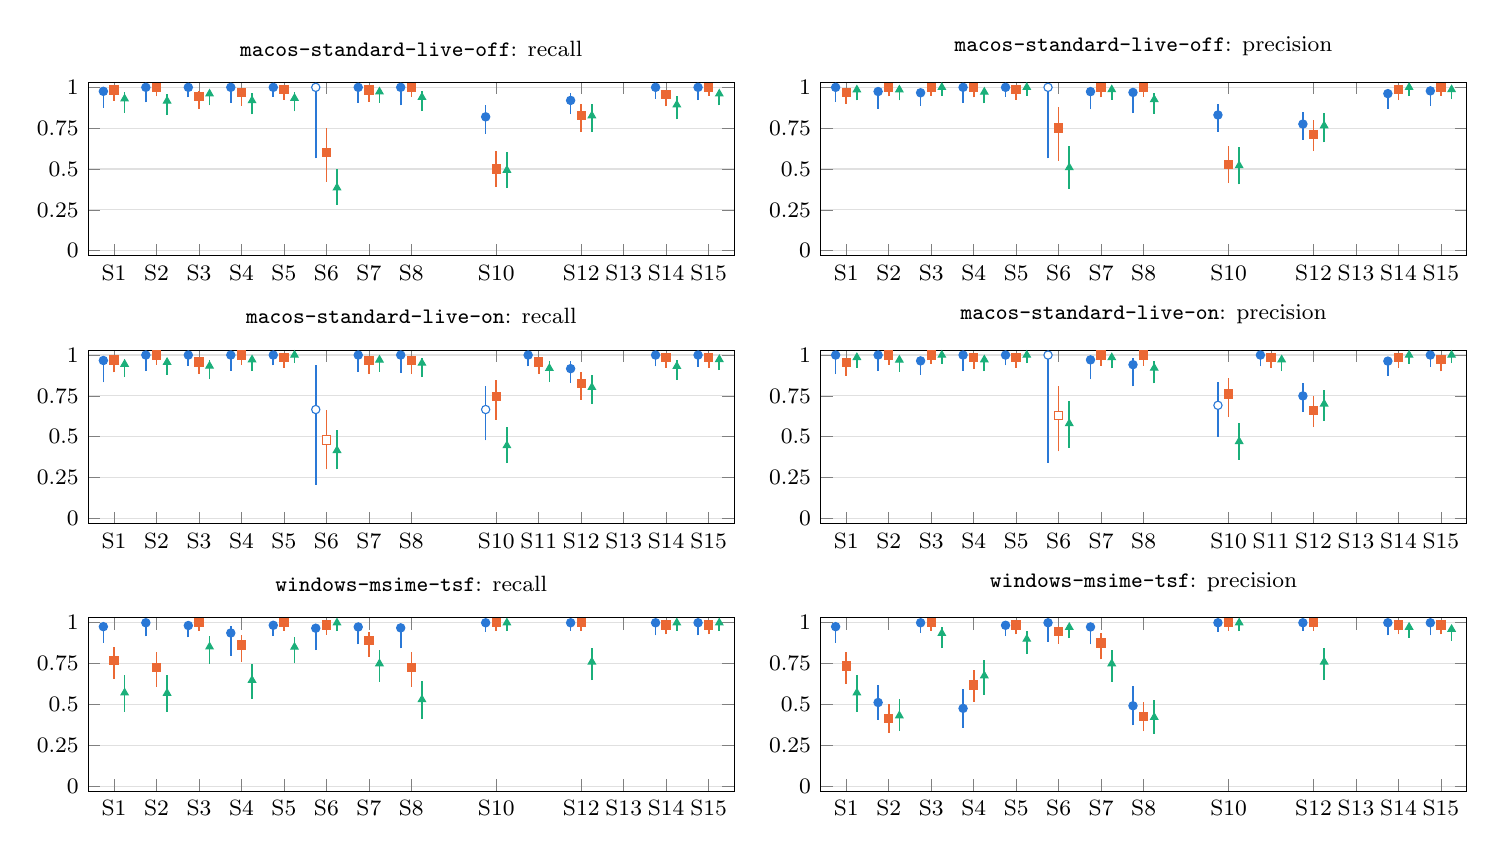
\begin{tikzpicture}
\begin{groupplot}[group style={group size=2 by 3, horizontal sep=1.1cm, vertical sep=1.2cm}, fig panel, fig proportion, scale only axis, width=8.2cm, height=2.2cm]
\nextgroupplot[xtick={1,2,3,4,5,6,7,8,10,12,13,14,15}, xticklabels={S1,S2,S3,S4,S5,S6,S7,S8,S10,S12,S13,S14,S15}, xmin=0.4, xmax=15.6, title={\texttt{macos-standard-live-off}: recall}, legend to name=fig:detection:legend, legend columns=4]
\addlegendimage{fig slow, fig point}
\addlegendentry{slow}
\addlegendimage{fig mid, fig point}
\addlegendentry{mid}
\addlegendimage{fig fast, fig point}
\addlegendentry{fast}
\addlegendimage{black, mark=*, fig point, fig open}
\addlegendentry{fewer than 30 trials}
\addplot[forget plot, fig interval, fig slow] table[row sep=\\] {x y\\0.75 0.874049\\0.75 0.995681\\0.75 nan\\1.75 0.90819\\1.75 1\\1.75 nan\\2.75 0.937882\\2.75 1\\2.75 nan\\3.75 0.905942\\3.75 1\\3.75 nan\\4.75 0.943376\\4.75 1\\4.75 nan\\5.75 0.565518\\5.75 1\\5.75 nan\\6.75 0.905942\\6.75 1\\6.75 nan\\7.75 0.889745\\7.75 1\\7.75 nan\\9.75 0.715197\\9.75 0.891332\\9.75 nan\\11.75 0.836252\\11.75 0.96282\\11.75 nan\\13.75 0.928652\\13.75 1\\13.75 nan\\14.75 0.921348\\14.75 1\\14.75 nan\\};
\addplot[forget plot, fig slow, fig point] table[row sep=\\] {x y\\0.75 0.97561\\1.75 1\\2.75 1\\3.75 1\\4.75 1\\6.75 1\\7.75 1\\9.75 0.819444\\11.75 0.92\\13.75 1\\14.75 1\\};
\addplot[forget plot, fig slow, fig point, fig open] table[row sep=\\] {x y\\5.75 1\\};
\addplot[forget plot, fig interval, fig mid] table[row sep=\\] {x y\\1 0.919041\\1 0.99732\\1 nan\\2 0.944198\\2 1\\2 nan\\3 0.86741\\3 0.978488\\3 nan\\4 0.886362\\4 0.990811\\4 nan\\5 0.924439\\5 0.997509\\5 nan\\6 0.423204\\6 0.754094\\6 nan\\7 0.911449\\7 0.997052\\7 nan\\8 0.943376\\8 1\\8 nan\\10 0.388926\\10 0.611074\\10 nan\\12 0.725692\\12 0.895809\\12 nan\\14 0.882976\\14 0.985527\\14 nan\\15 0.950008\\15 1\\15 nan\\};
\addplot[forget plot, fig mid, fig point] table[row sep=\\] {x y\\1 0.984848\\2 1\\3 0.945205\\4 0.966667\\5 0.985915\\6 0.6\\7 0.983333\\8 1\\10 0.5\\12 0.826667\\14 0.957746\\15 1\\};
\addplot[forget plot, fig interval, fig fast] table[row sep=\\] {x y\\1.25 0.84551\\1.25 0.969546\\1.25 nan\\2.25 0.829876\\2.25 0.961248\\2.25 nan\\3.25 0.88887\\3.25 0.986304\\3.25 nan\\4.25 0.834181\\4.25 0.96231\\4.25 nan\\5.25 0.853249\\5.25 0.97119\\5.25 nan\\6.25 0.280477\\6.25 0.502843\\6.25 nan\\7.25 0.905499\\7.25 0.992454\\7.25 nan\\8.25 0.854271\\8.25 0.976181\\8.25 nan\\10.25 0.3833\\10.25 0.604016\\10.25 nan\\12.25 0.725692\\12.25 0.895809\\12.25 nan\\14.25 0.803386\\14.25 0.944951\\14.25 nan\\15.25 0.88887\\15.25 0.986304\\15.25 nan\\};
\addplot[forget plot, fig fast, fig point] table[row sep=\\] {x y\\1.25 0.929577\\2.25 0.916667\\3.25 0.96\\4.25 0.918919\\5.25 0.933333\\6.25 0.385714\\7.25 0.972603\\8.25 0.939394\\10.25 0.493333\\12.25 0.826667\\14.25 0.893333\\15.25 0.96\\};
\nextgroupplot[xtick={1,2,3,4,5,6,7,8,10,12,13,14,15}, xticklabels={S1,S2,S3,S4,S5,S6,S7,S8,S10,S12,S13,S14,S15}, xmin=0.4, xmax=15.6, title={\texttt{macos-standard-live-off}: precision}]
\addplot[forget plot, fig interval, fig slow] table[row sep=\\] {x y\\0.75 0.912378\\0.75 1\\0.75 nan\\1.75 0.86819\\1.75 0.995459\\1.75 nan\\2.75 0.886362\\2.75 0.990811\\2.75 nan\\3.75 0.905942\\3.75 1\\3.75 nan\\4.75 0.943376\\4.75 1\\4.75 nan\\5.75 0.565518\\5.75 1\\5.75 nan\\6.75 0.865051\\6.75 0.995339\\6.75 nan\\7.75 0.842557\\7.75 0.994462\\7.75 nan\\9.75 0.727409\\9.75 0.900585\\9.75 nan\\11.75 0.678226\\11.75 0.849555\\11.75 nan\\13.75 0.870188\\13.75 0.989388\\13.75 nan\\14.75 0.886647\\14.75 0.996152\\14.75 nan\\};
\addplot[forget plot, fig slow, fig point] table[row sep=\\] {x y\\0.75 1\\1.75 0.974359\\2.75 0.966667\\3.75 1\\4.75 1\\6.75 0.973684\\7.75 0.96875\\9.75 0.830986\\11.75 0.775281\\13.75 0.961538\\14.75 0.978261\\};
\addplot[forget plot, fig slow, fig point, fig open] table[row sep=\\] {x y\\5.75 1\\};
\addplot[forget plot, fig interval, fig mid] table[row sep=\\] {x y\\1 0.897534\\1 0.991775\\1 nan\\2 0.944198\\2 1\\2 nan\\3 0.947263\\3 1\\3 nan\\4 0.937882\\4 1\\4 nan\\5 0.924439\\5 0.997509\\5 nan\\6 0.551006\\6 0.880006\\6 nan\\7 0.938871\\7 1\\7 nan\\8 0.943376\\8 1\\8 nan\\10 0.413219\\10 0.640951\\10 nan\\12 0.61016\\12 0.797143\\12 nan\\14 0.922369\\14 0.997437\\14 nan\\15 0.950008\\15 1\\15 nan\\};
\addplot[forget plot, fig mid, fig point] table[row sep=\\] {x y\\1 0.970149\\2 1\\3 1\\4 1\\5 0.985915\\6 0.75\\7 1\\8 1\\10 0.528571\\12 0.712644\\14 0.985507\\15 1\\};
\addplot[forget plot, fig interval, fig fast] table[row sep=\\] {x y\\1.25 0.920181\\1.25 0.99736\\1.25 nan\\2.25 0.920181\\2.25 0.99736\\2.25 nan\\3.25 0.949349\\3.25 1\\3.25 nan\\4.25 0.901677\\4.25 0.992129\\4.25 nan\\5.25 0.947977\\5.25 1\\5.25 nan\\6.25 0.378835\\6.25 0.638758\\6.25 nan\\7.25 0.925434\\7.25 0.997544\\7.25 nan\\8.25 0.83691\\8.25 0.967704\\8.25 nan\\10.25 0.40686\\10.25 0.633225\\10.25 nan\\12.25 0.662453\\12.25 0.844375\\12.25 nan\\14.25 0.945774\\14.25 1\\14.25 nan\\15.25 0.926403\\15.25 0.997578\\15.25 nan\\};
\addplot[forget plot, fig fast, fig point] table[row sep=\\] {x y\\1.25 0.985075\\2.25 0.985075\\3.25 1\\4.25 0.971429\\5.25 1\\6.25 0.509434\\7.25 0.986111\\8.25 0.925373\\10.25 0.521127\\12.25 0.765432\\14.25 1\\15.25 0.986301\\};
\nextgroupplot[xtick={1,2,3,4,5,6,7,8,10,11,12,13,14,15}, xticklabels={S1,S2,S3,S4,S5,S6,S7,S8,S10,S11,S12,S13,S14,S15}, xmin=0.4, xmax=15.6, title={\texttt{macos-standard-live-on}: recall}]
\addplot[forget plot, fig interval, fig slow] table[row sep=\\] {x y\\0.75 0.833296\\0.75 0.994091\\0.75 nan\\1.75 0.901099\\1.75 1\\1.75 nan\\2.75 0.933586\\2.75 1\\2.75 nan\\3.75 0.903581\\3.75 1\\3.75 nan\\4.75 0.936861\\4.75 1\\4.75 nan\\5.75 0.20766\\5.75 0.938508\\5.75 nan\\6.75 0.89573\\6.75 1\\6.75 nan\\7.75 0.892821\\7.75 1\\7.75 nan\\9.75 0.478248\\9.75 0.813567\\9.75 nan\\10.75 0.931208\\10.75 1\\10.75 nan\\11.75 0.829876\\11.75 0.961248\\11.75 nan\\13.75 0.931208\\13.75 1\\13.75 nan\\14.75 0.927302\\14.75 1\\14.75 nan\\};
\addplot[forget plot, fig slow, fig point] table[row sep=\\] {x y\\0.75 0.966667\\1.75 1\\2.75 1\\3.75 1\\4.75 1\\6.75 1\\7.75 1\\10.75 1\\11.75 0.916667\\13.75 1\\14.75 1\\};
\addplot[forget plot, fig slow, fig point, fig open] table[row sep=\\] {x y\\5.75 0.666667\\9.75 0.666667\\};
\addplot[forget plot, fig interval, fig mid] table[row sep=\\] {x y\\1 0.894573\\1 0.991521\\1 nan\\2 0.939828\\2 1\\2 nan\\3 0.882976\\3 0.985527\\3 nan\\4 0.940756\\4 1\\4 nan\\5 0.923418\\5 0.997474\\5 nan\\6 0.300313\\6 0.665015\\6 nan\\7 0.882709\\7 0.990492\\7 nan\\8 0.882709\\8 0.990492\\8 nan\\10 0.604918\\10 0.847468\\10 nan\\11 0.882976\\11 0.985527\\11 nan\\12 0.725692\\12 0.895809\\12 nan\\14 0.923418\\14 0.997474\\14 nan\\15 0.92129\\15 0.997399\\15 nan\\};
\addplot[forget plot, fig mid, fig point] table[row sep=\\] {x y\\1 0.969231\\2 1\\3 0.957746\\4 1\\5 0.985714\\7 0.965517\\8 0.965517\\10 0.744681\\11 0.957746\\12 0.826667\\14 0.985714\\15 0.985294\\};
\addplot[forget plot, fig mid, fig point, fig open] table[row sep=\\] {x y\\6 0.48\\};
\addplot[forget plot, fig interval, fig fast] table[row sep=\\] {x y\\1.25 0.86568\\1.25 0.978186\\1.25 nan\\2.25 0.878128\\2.25 0.984883\\2.25 nan\\3.25 0.853249\\3.25 0.97119\\3.25 nan\\4.25 0.901677\\4.25 0.992129\\4.25 nan\\5.25 0.951276\\5.25 1\\5.25 nan\\6.25 0.300643\\6.25 0.542719\\6.25 nan\\7.25 0.897534\\7.25 0.991775\\7.25 nan\\8.25 0.865089\\8.25 0.983134\\8.25 nan\\10.25 0.338158\\10.25 0.559069\\10.25 nan\\11.25 0.834181\\11.25 0.96231\\11.25 nan\\12.25 0.699562\\12.25 0.87658\\12.25 nan\\14.25 0.849479\\14.25 0.970391\\14.25 nan\\15.25 0.907885\\15.25 0.992656\\15.25 nan\\};
\addplot[forget plot, fig fast, fig point] table[row sep=\\] {x y\\1.25 0.944444\\2.25 0.955882\\3.25 0.933333\\4.25 0.971429\\5.25 1\\6.25 0.416667\\7.25 0.970149\\8.25 0.95082\\10.25 0.445946\\11.25 0.918919\\12.25 0.802632\\14.25 0.931507\\15.25 0.973333\\};
\nextgroupplot[xtick={1,2,3,4,5,6,7,8,10,11,12,13,14,15}, xticklabels={S1,S2,S3,S4,S5,S6,S7,S8,S10,S11,S12,S13,S14,S15}, xmin=0.4, xmax=15.6, title={\texttt{macos-standard-live-on}: precision}]
\addplot[forget plot, fig interval, fig slow] table[row sep=\\] {x y\\0.75 0.88303\\0.75 1\\0.75 nan\\1.75 0.901099\\1.75 1\\1.75 nan\\2.75 0.878812\\2.75 0.990151\\2.75 nan\\3.75 0.903581\\3.75 1\\3.75 nan\\4.75 0.936861\\4.75 1\\4.75 nan\\5.75 0.34238\\5.75 1\\5.75 nan\\6.75 0.850844\\6.75 0.994789\\6.75 nan\\7.75 0.809064\\7.75 0.983717\\7.75 nan\\9.75 0.500117\\9.75 0.834987\\9.75 nan\\10.75 0.931208\\10.75 1\\10.75 nan\\11.75 0.65037\\11.75 0.828717\\11.75 nan\\13.75 0.874648\\13.75 0.989784\\13.75 nan\\14.75 0.927302\\14.75 1\\14.75 nan\\};
\addplot[forget plot, fig slow, fig point] table[row sep=\\] {x y\\0.75 1\\1.75 1\\2.75 0.964286\\3.75 1\\4.75 1\\6.75 0.970588\\7.75 0.941176\\10.75 1\\11.75 0.75\\13.75 0.962963\\14.75 1\\};
\addplot[forget plot, fig slow, fig point, fig open] table[row sep=\\] {x y\\5.75 1\\9.75 0.692308\\};
\addplot[forget plot, fig interval, fig mid] table[row sep=\\] {x y\\1 0.874667\\1 0.984422\\1 nan\\2 0.939828\\2 1\\2 nan\\3 0.946529\\3 1\\3 nan\\4 0.914133\\4 0.997147\\4 nan\\5 0.923418\\5 0.997474\\5 nan\\6 0.410395\\6 0.808505\\6 nan\\7 0.935806\\7 1\\7 nan\\8 0.935806\\8 1\\8 nan\\10 0.620649\\10 0.860878\\10 nan\\11 0.922369\\11 0.997437\\11 nan\\12 0.559208\\12 0.74741\\12 nan\\14 0.923418\\14 0.997474\\14 nan\\15 0.900334\\15 0.992015\\15 nan\\};
\addplot[forget plot, fig mid, fig point] table[row sep=\\] {x y\\1 0.954545\\2 1\\3 1\\4 0.983871\\5 0.985714\\7 1\\8 1\\10 0.76087\\11 0.985507\\12 0.659574\\14 0.985714\\15 0.971014\\};
\addplot[forget plot, fig mid, fig point, fig open] table[row sep=\\] {x y\\6 0.631579\\};
\addplot[forget plot, fig interval, fig fast] table[row sep=\\] {x y\\1.25 0.922369\\1.25 0.997437\\1.25 nan\\2.25 0.897534\\2.25 0.991775\\2.25 nan\\3.25 0.947977\\3.25 1\\3.25 nan\\4.25 0.901677\\4.25 0.992129\\4.25 nan\\5.25 0.951276\\5.25 1\\5.25 nan\\6.25 0.433286\\6.25 0.716154\\6.25 nan\\7.25 0.919041\\7.25 0.99732\\7.25 nan\\8.25 0.827297\\8.25 0.965624\\8.25 nan\\10.25 0.359049\\10.25 0.586781\\10.25 nan\\11.25 0.901677\\11.25 0.992129\\11.25 nan\\12.25 0.598128\\12.25 0.787159\\12.25 nan\\14.25 0.946529\\14.25 1\\14.25 nan\\15.25 0.950008\\15.25 1\\15.25 nan\\};
\addplot[forget plot, fig fast, fig point] table[row sep=\\] {x y\\1.25 0.985507\\2.25 0.970149\\3.25 1\\4.25 0.971429\\5.25 1\\6.25 0.581395\\7.25 0.984848\\8.25 0.920635\\10.25 0.471429\\11.25 0.971429\\12.25 0.701149\\14.25 1\\15.25 1\\};
\nextgroupplot[xtick={1,2,3,4,5,6,7,8,10,12,13,14,15}, xticklabels={S1,S2,S3,S4,S5,S6,S7,S8,S10,S12,S13,S14,S15}, xmin=0.4, xmax=15.6, title={\texttt{windows-msime-tsf}: recall}]
\addplot[forget plot, fig interval, fig slow] table[row sep=\\] {x y\\0.75 0.876788\\0.75 0.995785\\0.75 nan\\1.75 0.916201\\1.75 1\\1.75 nan\\2.75 0.910043\\2.75 0.997002\\2.75 nan\\3.75 0.798529\\3.75 0.982689\\3.75 nan\\4.75 0.917867\\4.75 0.997279\\4.75 nan\\5.75 0.833296\\5.75 0.994091\\5.75 nan\\6.75 0.86819\\6.75 0.995459\\6.75 nan\\7.75 0.842557\\7.75 0.994462\\7.75 nan\\9.75 0.944997\\9.75 1\\9.75 nan\\11.75 0.951276\\11.75 1\\11.75 nan\\13.75 0.922926\\13.75 1\\13.75 nan\\14.75 0.922926\\14.75 1\\14.75 nan\\};
\addplot[forget plot, fig slow, fig point] table[row sep=\\] {x y\\0.75 0.97619\\1.75 1\\2.75 0.983051\\3.75 0.9375\\4.75 0.984615\\5.75 0.966667\\6.75 0.974359\\7.75 0.96875\\9.75 1\\11.75 1\\13.75 1\\14.75 1\\};
\addplot[forget plot, fig interval, fig mid] table[row sep=\\] {x y\\1 0.656032\\1 0.851921\\1 nan\\2 0.609578\\2 0.819967\\2 nan\\3 0.951276\\3 1\\3 nan\\4 0.760704\\4 0.926567\\4 nan\\5 0.951276\\5 1\\5 nan\\6 0.926403\\6 0.997578\\6 nan\\7 0.791014\\7 0.945999\\7 nan\\8 0.609578\\8 0.819967\\8 nan\\10 0.948672\\10 1\\10 nan\\12 0.951276\\12 1\\12 nan\\14 0.928266\\14 0.997642\\14 nan\\15 0.928266\\15 0.997642\\15 nan\\};
\addplot[forget plot, fig mid, fig point] table[row sep=\\] {x y\\1 0.768116\\2 0.727273\\3 1\\4 0.863636\\5 1\\6 0.986301\\7 0.890625\\8 0.727273\\10 1\\12 1\\14 0.986667\\15 0.986667\\};
\addplot[forget plot, fig interval, fig fast] table[row sep=\\] {x y\\1.25 0.454778\\1.25 0.680647\\1.25 nan\\2.25 0.454433\\2.25 0.677421\\2.25 nan\\3.25 0.750026\\3.25 0.918112\\3.25 nan\\4.25 0.535008\\4.25 0.747618\\4.25 nan\\5.25 0.753105\\5.25 0.914919\\5.25 nan\\6.25 0.948672\\6.25 1\\6.25 nan\\7.25 0.639065\\7.25 0.835609\\7.25 nan\\8.25 0.411577\\8.25 0.645696\\8.25 nan\\10.25 0.949349\\10.25 1\\10.25 nan\\12.25 0.649588\\12.25 0.844791\\12.25 nan\\14.25 0.950008\\14.25 1\\14.25 nan\\15.25 0.950008\\15.25 1\\15.25 nan\\};
\addplot[forget plot, fig fast, fig point] table[row sep=\\] {x y\\1.25 0.571429\\2.25 0.569444\\3.25 0.852941\\4.25 0.648649\\5.25 0.851351\\6.25 1\\7.25 0.75\\8.25 0.530303\\10.25 1\\12.25 0.760563\\14.25 1\\15.25 1\\};
\nextgroupplot[xtick={1,2,3,4,5,6,7,8,10,12,13,14,15}, xticklabels={S1,S2,S3,S4,S5,S6,S7,S8,S10,S12,S13,S14,S15}, xmin=0.4, xmax=15.6, title={\texttt{windows-msime-tsf}: precision}]
\addplot[forget plot, fig interval, fig slow] table[row sep=\\] {x y\\0.75 0.876788\\0.75 0.995785\\0.75 nan\\1.75 0.405908\\1.75 0.617391\\1.75 nan\\2.75 0.937882\\2.75 1\\2.75 nan\\3.75 0.357821\\3.75 0.597296\\3.75 nan\\4.75 0.917867\\4.75 0.997279\\4.75 nan\\5.75 0.88303\\5.75 1\\5.75 nan\\6.75 0.86819\\6.75 0.995459\\6.75 nan\\7.75 0.372668\\7.75 0.612371\\7.75 nan\\9.75 0.944997\\9.75 1\\9.75 nan\\11.75 0.951276\\11.75 1\\11.75 nan\\13.75 0.922926\\13.75 1\\13.75 nan\\14.75 0.922926\\14.75 1\\14.75 nan\\};
\addplot[forget plot, fig slow, fig point] table[row sep=\\] {x y\\0.75 0.97619\\1.75 0.512195\\2.75 1\\3.75 0.47619\\4.75 0.984615\\5.75 1\\6.75 0.974359\\7.75 0.492063\\9.75 1\\11.75 1\\13.75 1\\14.75 1\\};
\addplot[forget plot, fig interval, fig mid] table[row sep=\\] {x y\\1 0.624241\\1 0.824062\\1 nan\\2 0.328335\\2 0.504778\\2 nan\\3 0.951276\\3 1\\3 nan\\4 0.517457\\4 0.712088\\4 nan\\5 0.929163\\5 0.997674\\5 nan\\6 0.872343\\6 0.979345\\6 nan\\7 0.775485\\7 0.936295\\7 nan\\8 0.337589\\8 0.516915\\8 nan\\10 0.948672\\10 1\\10 nan\\12 0.951276\\12 1\\12 nan\\14 0.928266\\14 0.997642\\14 nan\\15 0.928266\\15 0.997642\\15 nan\\};
\addplot[forget plot, fig mid, fig point] table[row sep=\\] {x y\\1 0.736111\\2 0.413793\\3 1\\4 0.619565\\5 0.986842\\6 0.947368\\7 0.876923\\8 0.424779\\10 1\\12 1\\14 0.986667\\15 0.986667\\};
\addplot[forget plot, fig interval, fig fast] table[row sep=\\] {x y\\1.25 0.454778\\1.25 0.680647\\1.25 nan\\2.25 0.336558\\2.25 0.531918\\2.25 nan\\3.25 0.845525\\3.25 0.974627\\3.25 nan\\4.25 0.560612\\4.25 0.773428\\4.25 nan\\5.25 0.807671\\5.25 0.950711\\5.25 nan\\6.25 0.905499\\6.25 0.992454\\6.25 nan\\7.25 0.639065\\7.25 0.835609\\7.25 nan\\8.25 0.32123\\8.25 0.529072\\8.25 nan\\10.25 0.949349\\10.25 1\\10.25 nan\\12.25 0.649588\\12.25 0.844791\\12.25 nan\\14.25 0.907885\\14.25 0.992656\\14.25 nan\\15.25 0.890252\\15.25 0.986485\\15.25 nan\\};
\addplot[forget plot, fig fast, fig point] table[row sep=\\] {x y\\1.25 0.571429\\2.25 0.431579\\3.25 0.935484\\4.25 0.676056\\5.25 0.9\\6.25 0.972603\\7.25 0.75\\8.25 0.421687\\10.25 1\\12.25 0.760563\\14.25 0.973333\\15.25 0.960526\\};
\end{groupplot}
\end{tikzpicture}
\caption{Recall and precision of the session rows against the reference per scenario and speed, with 95\% Wilson intervals, per cell, in the primary comparison (\texttt{gt\_obs}) and scope (\texttt{under\_limit}). Open marks: strata that keep fewer than 30 trials in the scope, which the ranges given in the text leave out. A stratum with no trial or no value in the scope is not drawn; Table~\ref{tab:detection} and the supplement give every stratum}
\label{fig:detection}
\end{sidewaysfigure}


\subsection{Per-session agreement}
\label{sec:results-session}

Over the matched sessions of the primary scope, the per-speed intervals of the bias of \texttt{dwell\_ms} against the
duration of the reference session spanned \rv{macos-standard-live-off.primary.dwellbias.range} with live conversion
off, \rv{macos-standard-live-on.primary.dwellbias.range} with it on, and \rv{windows-msime-tsf.primary.dwellbias.range}
on Windows; over all trials, \rv{macos-standard-live-off.all.dwellbias.range},
\rv{macos-standard-live-on.all.dwellbias.range} and \rv{windows-msime-tsf.all.dwellbias.range}. A negative bias means
that the logger's duration was shorter than the reference's. Table~\ref{tab:session} gives the bias, the limits of
agreement and the median absolute difference per speed, with the agreement of \texttt{abandon} and \texttt{nav};
Figure~\ref{fig:dwell} shows the bias and the limits of agreement per stratum, and the supplement gives every stratum
and the comparisons with the prediction.

The agreement of \texttt{abandon} with the outcome of the session was, pooled over the primary scope, for the sessions
whose commit was followed by a continuation, \rv{macos-standard-live-on.abandon.continued.with.primary} with live
conversion on, and for the other sessions \rv{macos-standard-live-off.abandon.continued.without.primary} with live
conversion off, \rv{macos-standard-live-on.abandon.continued.without.primary} with it on and
\rv{windows-msime-tsf.abandon.continued.without.primary} on Windows; with live conversion off and on Windows no session
had a continued commit. On Windows \texttt{nav} and \texttt{abandon} count presses system-wide while a session is open,
so they are upper bounds; in this design only the executor typed.

% Generated by manuscript/tools/results_tables.py from the result files; do not edit by hand.
\begin{sidewaystable}[p]
\caption{Per-session agreement per cell and speed, primary scope: the difference of \texttt{dwell\_ms} from the duration of the reference session (bias with its interval, limits of agreement, median absolute difference), the agreement of \texttt{abandon} with the outcome of the session (raw agreement and kappa), and the exact agreement of \texttt{nav} with the arrow presses sent; Pairs is the number of matched sessions; --: no value in the result file}
\label{tab:session}
\begin{tabular}{L{0.14}L{0.07}L{0.07}L{0.17}L{0.15}L{0.08}L{0.11}L{0.12}L{0.09}}
\toprule
Cell & Speed & Pairs & Bias (ms) & Limits (ms) & Median absolute difference (ms) & \texttt{abandon} agreement & \texttt{abandon} kappa & \texttt{nav} exact \\
\midrule
macos-standard-live-off & slow & 533 & $-$427 [$-$561, $-$300] & $-$3,236, 2,382 & 36 & 0.991 [0.978, 0.996] & 0.970 [0.945, 0.993] & 0.996 [0.986, 0.999] \\
 & mid & 708 & $-$2 [$-$76, 80] & $-$2,213, 2,208 & 39 & 0.980 [0.967, 0.988] & 0.937 [0.902, 0.968] & 0.999 [0.992, 1.000] \\
 & fast & 740 & 124 [53, 201] & $-$2,034, 2,283 & 44 & 0.969 [0.954, 0.979] & 0.906 [0.866, 0.941] & 1.000 [0.995, 1.000] \\
macos-standard-live-on & slow & 515 & $-$544 [$-$656, $-$447] & $-$3,010, 1,922 & 384 & 0.996 [0.986, 0.999] & 0.987 [0.967, 1.000] & 1.000 [0.993, 1.000] \\
 & mid & 746 & $-$82 [$-$165, 14] & $-$2,378, 2,215 & 171 & 0.985 [0.974, 0.992] & 0.951 [0.923, 0.974] & 0.996 [0.988, 0.999] \\
 & fast & 797 & 86 [15, 156] & $-$2,059, 2,230 & 97 & 0.971 [0.957, 0.981] & 0.909 [0.869, 0.944] & 0.999 [0.993, 1.000] \\
windows-msime-tsf & slow & 566 & $-$934 [$-$1,055, $-$823] & $-$3,491, 1,623 & 480 & 0.896 [0.868, 0.918] & 0.629 [0.537, 0.717] & 1.000 [0.993, 1.000] \\
 & mid & 779 & $-$1,006 [$-$1,121, $-$892] & $-$4,321, 2,310 & 276 & 0.836 [0.808, 0.860] & 0.467 [0.409, 0.523] & 0.969 [0.955, 0.979] \\
 & fast & 682 & $-$550 [$-$654, $-$456] & $-$2,860, 1,760 & 178 & 0.824 [0.794, 0.851] & 0.431 [0.361, 0.504] & 0.921 [0.898, 0.939] \\
\bottomrule
\end{tabular}
\end{sidewaystable}

% Generated by manuscript/tools/results_tables.py from the result files; do not edit by hand.
\begin{figure}[p]
\centering
\pgfplotslegendfromname{fig:dwell:legend}\par\medskip
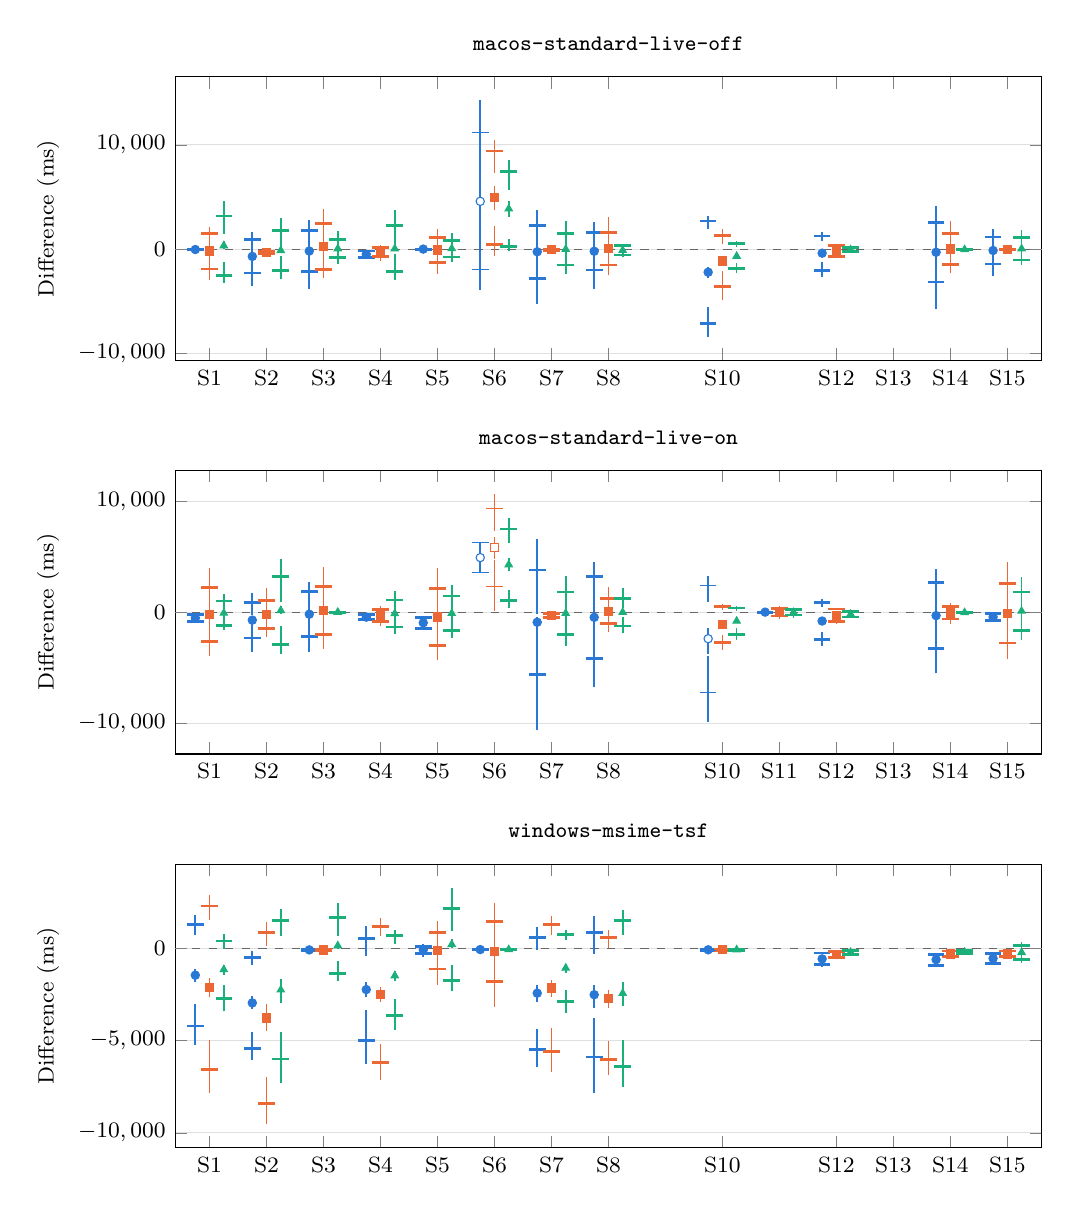
\begin{tikzpicture}
\begin{groupplot}[group style={group size=1 by 3, vertical sep=1.4cm}, fig panel, fig zero, scale only axis, width=11cm, height=3.6cm, ylabel={Difference (ms)}]
\nextgroupplot[xtick={1,2,3,4,5,6,7,8,10,12,13,14,15}, xticklabels={S1,S2,S3,S4,S5,S6,S7,S8,S10,S12,S13,S14,S15}, xmin=0.4, xmax=15.6, title={\texttt{macos-standard-live-off}}, legend to name=fig:dwell:legend, legend columns=5]
\addlegendimage{fig slow, fig point}
\addlegendentry{slow}
\addlegendimage{fig mid, fig point}
\addlegendentry{mid}
\addlegendimage{fig fast, fig point}
\addlegendentry{fast}
\addlegendimage{black, mark=*, fig point, fig open}
\addlegendentry{fewer than 30 trials}
\addlegendimage{black, fig limit}
\addlegendentry{limit of agreement}
\addplot[forget plot, fig interval, fig slow] table[row sep=\\] {x y\\0.75 -75.4257\\0.75 -59.8758\\0.75 nan\\1.75 -3576.2\\1.75 -788.026\\1.75 nan\\2.75 -3836.69\\2.75 -12.8138\\2.75 nan\\3.75 -964.032\\3.75 -673.412\\3.75 nan\\4.75 -2.77561\\4.75 -1.15887\\4.75 nan\\5.75 -3894.67\\5.75 2428.29\\5.75 nan\\6.75 -5294.56\\6.75 -58.5008\\6.75 nan\\7.75 -3803.61\\7.75 -62.4587\\7.75 nan\\9.75 -8392.22\\9.75 -5524.22\\9.75 nan\\11.75 -2688.81\\11.75 -1211.37\\11.75 nan\\13.75 -5732.33\\13.75 -60.6085\\13.75 nan\\14.75 -2605.38\\14.75 -51.3518\\14.75 nan\\};
\addplot[forget plot, fig slow, fig limit] table[row sep=\\] {x y\\0.75 -67.9431\\1.75 -2287.54\\2.75 -2154.02\\3.75 -819.049\\4.75 -2.02907\\6.75 -2806.82\\7.75 -1998.27\\9.75 -7109.15\\11.75 -2020.98\\13.75 -3158.57\\14.75 -1421.75\\};
\addplot[forget plot, fig slow, fig limit, fig open] table[row sep=\\] {x y\\5.75 -1993.26\\};
\addplot[forget plot, fig interval, fig mid] table[row sep=\\] {x y\\1 -2972.49\\1 -79.9924\\1 nan\\2 -439.694\\2 -378.312\\2 nan\\3 -2770.1\\3 -13.2494\\3 nan\\4 -1118.01\\4 -359.053\\4 nan\\5 -2405.32\\5 -0.811858\\5 nan\\6 -664.863\\6 2212.17\\6 nan\\7 -106.049\\7 -82.7035\\7 nan\\8 -2509.56\\8 -76.4093\\8 nan\\10 -4917.99\\10 -2130.87\\10 nan\\12 -838.405\\12 -526.477\\12 nan\\14 -2322.07\\14 -63.3582\\14 nan\\15 -78.9387\\15 -62.4595\\15 nan\\};
\addplot[forget plot, fig mid, fig limit] table[row sep=\\] {x y\\1 -1910.67\\2 -410.282\\3 -1978.41\\4 -722.404\\5 -1285.46\\6 434.382\\7 -95.1332\\8 -1516.85\\10 -3585.63\\12 -693.272\\14 -1480.26\\15 -71.0878\\};
\addplot[forget plot, fig interval, fig fast] table[row sep=\\] {x y\\1.25 -3240.45\\1.25 -1270.83\\1.25 nan\\2.25 -2882.41\\2.25 -611.772\\2.25 nan\\3.25 -1400.12\\3.25 -10.1817\\3.25 nan\\4.25 -3004.22\\4.25 -434.894\\4.25 nan\\5.25 -1257.83\\5.25 -1.61752\\5.25 nan\\6.25 -137.645\\6.25 989.54\\6.25 nan\\7.25 -2394.05\\7.25 -84.8501\\7.25 nan\\8.25 -789.422\\8.25 -264.137\\8.25 nan\\10.25 -2334.04\\10.25 -1343.92\\10.25 nan\\12.25 -354.956\\12.25 -158.428\\12.25 nan\\14.25 -86.7069\\14.25 -64.9602\\14.25 nan\\15.25 -1507.34\\15.25 -82.4561\\15.25 nan\\};
\addplot[forget plot, fig fast, fig limit] table[row sep=\\] {x y\\1.25 -2513.5\\2.25 -2015.25\\3.25 -810.647\\4.25 -2163.62\\5.25 -745.711\\6.25 280.151\\7.25 -1517.85\\8.25 -569.181\\10.25 -1880.23\\12.25 -261.718\\14.25 -76.4071\\15.25 -1038.1\\};
\addplot[forget plot, fig interval, fig slow] table[row sep=\\] {x y\\0.75 -13.412\\0.75 -0.642795\\0.75 nan\\1.75 -323.458\\1.75 1684.76\\1.75 nan\\2.75 3.33828\\2.75 2827.45\\2.75 nan\\3.75 -282.32\\3.75 -111.802\\3.75 nan\\4.75 6.77156\\4.75 9.29739\\4.75 nan\\5.75 4194.42\\5.75 14261.1\\5.75 nan\\6.75 -18.6951\\6.75 3774.95\\6.75 nan\\7.75 -16.85\\7.75 2589.25\\7.75 nan\\9.75 1962.02\\9.75 3136.11\\9.75 nan\\11.75 767.877\\11.75 1612.04\\11.75 nan\\13.75 -13.9135\\13.75 4150.09\\13.75 nan\\14.75 -8.87406\\14.75 1914.6\\14.75 nan\\};
\addplot[forget plot, fig slow, fig limit] table[row sep=\\] {x y\\0.75 -6.25687\\1.75 892.326\\2.75 1787.95\\3.75 -187.978\\4.75 8.09157\\6.75 2301.69\\7.75 1589.24\\9.75 2689.59\\11.75 1249.73\\13.75 2562.29\\14.75 1163.53\\};
\addplot[forget plot, fig slow, fig limit, fig open] table[row sep=\\] {x y\\5.75 11162.5\\};
\addplot[forget plot, fig interval, fig mid] table[row sep=\\] {x y\\1 -6.68885\\1 2162.89\\1 nan\\2 -206.785\\2 -159.064\\2 nan\\3 3.86477\\3 3864.68\\3 nan\\4 -121.668\\4 438.616\\4 nan\\5 7.36715\\5 1927.08\\5 nan\\6 7294.19\\6 10499.4\\6 nan\\7 -12.9216\\7 -1.07384\\7 nan\\8 -11.6563\\8 3070.02\\8 nan\\10 456.75\\10 1885.67\\10 nan\\12 302.333\\12 395.724\\12 nan\\14 -10.4648\\14 2707.85\\14 nan\\15 -4.73687\\15 6.84323\\15 nan\\};
\addplot[forget plot, fig mid, fig limit] table[row sep=\\] {x y\\1 1514.73\\2 -180.395\\3 2443.69\\4 172.266\\5 1144.74\\6 9421.06\\7 -6.121\\8 1628.16\\10 1293.79\\12 355.369\\14 1526.32\\15 1.27954\\};
\addplot[forget plot, fig interval, fig fast] table[row sep=\\] {x y\\1.25 1416.47\\1.25 4654.97\\1.25 nan\\2.25 205.487\\2.25 2964.85\\2.25 nan\\3.25 2.88371\\3.25 1751.37\\3.25 nan\\4.25 164.044\\4.25 3728.3\\4.25 nan\\5.25 7.58424\\5.25 1582.62\\5.25 nan\\6.25 5719.14\\6.25 8562.06\\6.25 nan\\7.25 -4.91843\\7.25 2683.6\\7.25 nan\\8.25 145.743\\8.25 460.264\\8.25 nan\\10.25 204.319\\10.25 740.427\\10.25 nan\\12.25 92.3654\\12.25 191.194\\12.25 nan\\14.25 -11.3952\\14.25 0.945151\\14.25 nan\\15.25 6.12604\\15.25 1872.08\\15.25 nan\\};
\addplot[forget plot, fig fast, fig limit] table[row sep=\\] {x y\\1.25 3185.1\\2.25 1760.49\\3.25 905.702\\4.25 2244.79\\5.25 848.397\\6.25 7466.22\\7.25 1495.17\\8.25 352.536\\10.25 521.256\\12.25 150.331\\14.25 -4.69736\\15.25 1115.94\\};
\addplot[forget plot, fig interval, fig slow] table[row sep=\\] {x y\\0.75 -41.9737\\0.75 -32.7672\\0.75 nan\\1.75 -954.087\\1.75 -538.251\\1.75 nan\\2.75 -513.473\\2.75 -4.19603\\2.75 nan\\3.75 -558.447\\3.75 -459.99\\3.75 nan\\4.75 2.4444\\4.75 3.70973\\4.75 nan\\5.75 2115\\5.75 7430.4\\5.75 nan\\6.75 -758.786\\6.75 -35.7937\\6.75 nan\\7.75 -603.683\\7.75 -36.0348\\7.75 nan\\9.75 -2794.1\\9.75 -1667.73\\9.75 nan\\11.75 -578.057\\11.75 -209.91\\11.75 nan\\13.75 -800.541\\13.75 -36.1997\\13.75 nan\\14.75 -343.785\\14.75 -28.1552\\14.75 nan\\};
\addplot[forget plot, fig slow, fig point] table[row sep=\\] {x y\\0.75 -37.1\\1.75 -697.605\\2.75 -183.034\\3.75 -503.514\\4.75 3.03125\\6.75 -252.568\\7.75 -204.516\\9.75 -2209.78\\11.75 -385.623\\13.75 -298.14\\14.75 -129.111\\};
\addplot[forget plot, fig slow, fig point, fig open] table[row sep=\\] {x y\\5.75 4584.6\\};
\addplot[forget plot, fig interval, fig mid] table[row sep=\\] {x y\\1 -406.395\\1 -41.8191\\1 nan\\2 -310.387\\2 -281.899\\2 nan\\3 -4.4834\\3 546.037\\3 nan\\4 -341.544\\4 -234.705\\4 nan\\5 -239.629\\5 4.4413\\5 nan\\6 3721.54\\6 6027.54\\6 nan\\7 -57.3224\\7 -44.6816\\7 nan\\8 -47.8659\\8 283.296\\8 nan\\10 -1602.61\\10 -765.282\\10 nan\\12 -237.873\\12 -108.499\\12 nan\\14 -116.424\\14 224.968\\14 nan\\15 -38.7015\\15 -31.1579\\15 nan\\};
\addplot[forget plot, fig mid, fig point] table[row sep=\\] {x y\\1 -197.969\\2 -295.338\\3 232.638\\4 -275.069\\5 -70.3571\\6 4927.72\\7 -50.6271\\8 55.6562\\10 -1145.92\\12 -168.952\\14 23.0294\\15 -34.9041\\};
\addplot[forget plot, fig interval, fig fast] table[row sep=\\] {x y\\1.25 38.2498\\1.25 737.143\\1.25 nan\\2.25 -332.022\\2.25 135.984\\2.25 nan\\3.25 -4.82098\\3.25 175.826\\3.25 nan\\4.25 -222.985\\4.25 392.617\\4.25 nan\\5.25 2.11756\\5.25 161.74\\5.25 nan\\6.25 3128.36\\6.25 4595.39\\6.25 nan\\7.25 -162.619\\7.25 209.03\\7.25 nan\\8.25 -166.715\\8.25 -59.6044\\8.25 nan\\10.25 -854.881\\10.25 -516.976\\10.25 nan\\12.25 -83.8848\\12.25 -32.8201\\12.25 nan\\14.25 -45.2723\\14.25 -36.127\\14.25 nan\\15.25 -62.9379\\15.25 185.441\\15.25 nan\\};
\addplot[forget plot, fig fast, fig point] table[row sep=\\] {x y\\1.25 335.803\\2.25 -127.379\\3.25 47.5278\\4.25 40.5882\\5.25 51.3429\\6.25 3873.19\\7.25 -11.338\\8.25 -108.323\\10.25 -679.486\\12.25 -55.6935\\14.25 -40.5522\\15.25 38.9167\\};
\nextgroupplot[xtick={1,2,3,4,5,6,7,8,10,11,12,13,14,15}, xticklabels={S1,S2,S3,S4,S5,S6,S7,S8,S10,S11,S12,S13,S14,S15}, xmin=0.4, xmax=15.6, title={\texttt{macos-standard-live-on}}]
\addplot[forget plot, fig interval, fig slow] table[row sep=\\] {x y\\0.75 -873.435\\0.75 -692.706\\0.75 nan\\1.75 -3608.8\\1.75 -841.39\\1.75 nan\\2.75 -3609.83\\2.75 0.925872\\2.75 nan\\3.75 -735.425\\3.75 -601.597\\3.75 nan\\4.75 -1585.2\\4.75 -1266.31\\4.75 nan\\5.75 3558.84\\5.75 5441\\5.75 nan\\6.75 -10648.3\\6.75 -782.136\\6.75 nan\\7.75 -6731.16\\7.75 -28.7168\\7.75 nan\\9.75 -9861.04\\9.75 -3965.87\\9.75 nan\\10.75 -0.0710007\\10.75 7.13739\\10.75 nan\\11.75 -3015.48\\11.75 -1741.03\\11.75 nan\\13.75 -5499.06\\13.75 -32.0094\\13.75 nan\\14.75 -777.752\\14.75 -631.646\\14.75 nan\\};
\addplot[forget plot, fig slow, fig limit] table[row sep=\\] {x y\\0.75 -790.628\\1.75 -2318.14\\2.75 -2207.77\\3.75 -674.02\\4.75 -1426.83\\6.75 -5601.26\\7.75 -4132.81\\10.75 2.70404\\11.75 -2444.22\\13.75 -3245.5\\14.75 -713.537\\};
\addplot[forget plot, fig slow, fig limit, fig open] table[row sep=\\] {x y\\5.75 3558.84\\9.75 -7193.06\\};
\addplot[forget plot, fig interval, fig mid] table[row sep=\\] {x y\\1 -3928.74\\1 -444.483\\1 nan\\2 -2187.2\\2 -403.273\\2 nan\\3 -3277.53\\3 7.00048\\3 nan\\4 -1257.16\\4 -372.561\\4 nan\\5 -4328.67\\5 -720.59\\5 nan\\6 145.781\\6 4759.39\\6 nan\\7 -481.143\\7 -379.439\\7 nan\\8 -1771.11\\8 6.98174\\8 nan\\10 -3396.92\\10 -2012.46\\10 nan\\11 -617.814\\11 7.19952\\11 nan\\12 -1047.2\\12 -650.411\\12 nan\\14 -1091.79\\14 -36.4524\\14 nan\\15 -4213.19\\15 -269.426\\15 nan\\};
\addplot[forget plot, fig mid, fig limit] table[row sep=\\] {x y\\1 -2625.34\\2 -1437.91\\3 -2026.55\\4 -806.574\\5 -2984.39\\7 -433.86\\8 -1036.61\\10 -2746.13\\11 -338.866\\12 -853.391\\14 -604.298\\15 -2769.31\\};
\addplot[forget plot, fig mid, fig limit, fig open] table[row sep=\\] {x y\\6 2333.51\\};
\addplot[forget plot, fig interval, fig fast] table[row sep=\\] {x y\\1.25 -1556.3\\1.25 -236.17\\1.25 nan\\2.25 -3781.89\\2.25 -1256.47\\2.25 nan\\3.25 2.73516\\3.25 9.24333\\3.25 nan\\4.25 -1966.44\\4.25 -188.299\\4.25 nan\\5.25 -2297.1\\5.25 -315.466\\5.25 nan\\6.25 427.68\\6.25 2010.63\\6.25 nan\\7.25 -3073.67\\7.25 -208.558\\7.25 nan\\8.25 -1874.8\\8.25 -387.284\\8.25 nan\\10.25 -2453.84\\10.25 -1392.57\\10.25 nan\\11.25 -464.789\\11.25 10.0144\\11.25 nan\\12.25 -501.712\\12.25 -347.696\\12.25 nan\\14.25 -49.3924\\14.25 -32.9736\\14.25 nan\\15.25 -2493.36\\15.25 -55.7979\\15.25 nan\\};
\addplot[forget plot, fig fast, fig limit] table[row sep=\\] {x y\\1.25 -1151.89\\2.25 -2900.12\\3.25 5.85425\\4.25 -1316.89\\5.25 -1652.65\\6.25 1080.21\\7.25 -2014.14\\8.25 -1231.62\\10.25 -1964.77\\11.25 -232.638\\12.25 -426.75\\14.25 -41.1769\\15.25 -1607.04\\};
\addplot[forget plot, fig interval, fig slow] table[row sep=\\] {x y\\0.75 -321.994\\0.75 -142.059\\0.75 nan\\1.75 -276.919\\1.75 1711.32\\1.75 nan\\2.75 43.7272\\2.75 2763.7\\2.75 nan\\3.75 -228.872\\3.75 -147.989\\3.75 nan\\4.75 -594.069\\4.75 -316.319\\4.75 nan\\5.75 4443\\5.75 6325.16\\5.75 nan\\6.75 -147.116\\6.75 6600.66\\6.75 nan\\7.75 51.4647\\7.75 4572.75\\7.75 nan\\9.75 895.596\\9.75 3272.73\\9.75 nan\\10.75 32.1682\\10.75 47.7098\\10.75 nan\\11.75 446.716\\11.75 1204.16\\11.75 nan\\13.75 36.9732\\13.75 3954.01\\13.75 nan\\14.75 -218.62\\14.75 -39.5392\\14.75 nan\\};
\addplot[forget plot, fig slow, fig limit] table[row sep=\\] {x y\\0.75 -224.613\\1.75 915.514\\2.75 1872.62\\3.75 -184.091\\4.75 -452.226\\6.75 3818.71\\7.75 3234.38\\10.75 40.796\\11.75 882.009\\13.75 2661.3\\14.75 -127.606\\};
\addplot[forget plot, fig slow, fig limit, fig open] table[row sep=\\] {x y\\5.75 6325.16\\9.75 2441.17\\};
\addplot[forget plot, fig interval, fig mid] table[row sep=\\] {x y\\1 7.8456\\1 3977.5\\1 nan\\2 -136.18\\2 2172.16\\2 nan\\3 31.9077\\3 4115.39\\3 nan\\4 -102.687\\4 551.166\\4 nan\\5 -220.639\\5 3976.61\\5 nan\\6 7318.87\\6 10670.1\\6 nan\\7 -131.974\\7 -47.1447\\7 nan\\8 29.7563\\8 2333.44\\8 nan\\10 197.878\\10 796.729\\10 nan\\11 31.6417\\11 533.042\\11 nan\\12 194.378\\12 393.548\\12 nan\\14 8.75325\\14 850.47\\14 nan\\15 51.1233\\15 4562.57\\15 nan\\};
\addplot[forget plot, fig mid, fig limit] table[row sep=\\] {x y\\1 2274.45\\2 1047.41\\3 2337.29\\4 249.295\\5 2160.54\\7 -88.1043\\8 1226.61\\10 546.874\\11 336.837\\12 302.424\\14 510.24\\15 2599.49\\};
\addplot[forget plot, fig mid, fig limit, fig open] table[row sep=\\] {x y\\6 9402.32\\};
\addplot[forget plot, fig interval, fig fast] table[row sep=\\] {x y\\1.25 -55.3667\\1.25 1697.18\\1.25 nan\\2.25 914.275\\2.25 4852.75\\2.25 nan\\3.25 30.4411\\3.25 39.9634\\3.25 nan\\4.25 -27.3712\\4.25 1968.61\\4.25 nan\\5.25 -132.852\\5.25 2508.36\\5.25 nan\\6.25 6304.77\\6.25 8540.72\\6.25 nan\\7.25 -66.0539\\7.25 3273.46\\7.25 nan\\8.25 355.123\\8.25 2224.44\\8.25 nan\\10.25 107.338\\10.25 617.09\\10.25 nan\\11.25 27.1612\\11.25 372.949\\11.25 nan\\12.25 68.5085\\12.25 145.199\\12.25 nan\\14.25 5.29311\\14.25 16.2495\\14.25 nan\\15.25 7.37004\\15.25 3184.44\\15.25 nan\\};
\addplot[forget plot, fig fast, fig limit] table[row sep=\\] {x y\\1.25 1021.27\\2.25 3236.09\\3.25 35.46\\4.25 1106.77\\5.25 1470.89\\6.25 7530.43\\7.25 1842.51\\8.25 1248.44\\10.25 403.138\\11.25 232.52\\12.25 112.225\\14.25 10.5592\\15.25 1833.45\\};
\addplot[forget plot, fig interval, fig slow] table[row sep=\\] {x y\\0.75 -557.975\\0.75 -452.883\\0.75 nan\\1.75 -973.598\\1.75 -527.987\\1.75 nan\\2.75 -424.479\\2.75 23.8962\\2.75 nan\\3.75 -466.548\\3.75 -394.27\\3.75 nan\\4.75 -1007.91\\4.75 -878.166\\4.75 nan\\5.75 4443\\5.75 5441\\5.75 nan\\6.75 -1975.92\\6.75 -428.51\\6.75 nan\\7.75 -1124.05\\7.75 12.7744\\7.75 nan\\9.75 -3777.06\\9.75 -1371.76\\9.75 nan\\10.75 18.8034\\10.75 25.0176\\10.75 nan\\11.75 -984.588\\11.75 -589.779\\11.75 nan\\13.75 -793.963\\13.75 3.68545\\13.75 nan\\14.75 -459.384\\14.75 -375.587\\14.75 nan\\};
\addplot[forget plot, fig slow, fig point] table[row sep=\\] {x y\\0.75 -507.621\\1.75 -701.314\\2.75 -167.574\\3.75 -429.056\\4.75 -939.526\\6.75 -891.273\\7.75 -449.219\\10.75 21.75\\11.75 -781.106\\13.75 -292.096\\14.75 -420.571\\};
\addplot[forget plot, fig slow, fig point, fig open] table[row sep=\\] {x y\\5.75 4942\\9.75 -2375.94\\};
\addplot[forget plot, fig interval, fig mid] table[row sep=\\] {x y\\1 -473.595\\1 161.111\\1 nan\\2 -294.287\\2 -8.03478\\2 nan\\3 18.875\\3 419.229\\3 nan\\4 -356.46\\4 -227.873\\4 nan\\5 -686.39\\5 -67.37\\5 nan\\6 4836.4\\6 6782.25\\6 nan\\7 -284.199\\7 -238.187\\7 nan\\8 16.2806\\8 281.092\\8 nan\\10 -1406.46\\10 -842.913\\10 nan\\11 -42.8777\\11 21.6305\\11 nan\\12 -351.808\\12 -204.527\\12 nan\\14 -121.395\\14 -10.3801\\14 nan\\15 -381.32\\15 267.675\\15 nan\\};
\addplot[forget plot, fig mid, fig point] table[row sep=\\] {x y\\1 -175.444\\2 -195.25\\3 155.368\\4 -278.639\\5 -411.928\\7 -260.982\\8 95\\10 -1099.63\\11 -1.01471\\12 -275.484\\14 -47.029\\15 -84.9104\\};
\addplot[forget plot, fig mid, fig point, fig open] table[row sep=\\] {x y\\6 5867.92\\};
\addplot[forget plot, fig interval, fig fast] table[row sep=\\] {x y\\1.25 -173.148\\1.25 71.5474\\1.25 nan\\2.25 -158.804\\2.25 564.006\\2.25 nan\\3.25 18.8665\\3.25 22.4219\\3.25 nan\\4.25 -241.417\\4.25 63.5504\\4.25 nan\\5.25 -227.632\\5.25 108.83\\5.25 nan\\6.25 3761.81\\6.25 4901.08\\6.25 nan\\7.25 -301.969\\7.25 175.28\\7.25 nan\\8.25 -123.296\\8.25 191.224\\8.25 nan\\10.25 -991.977\\10.25 -589.155\\10.25 nan\\11.25 -45.4222\\11.25 19.635\\11.25 nan\\12.25 -191.289\\12.25 -125.815\\12.25 nan\\14.25 -17.9105\\14.25 -12.5776\\14.25 nan\\15.25 -28.5069\\15.25 350.24\\15.25 nan\\};
\addplot[forget plot, fig fast, fig point] table[row sep=\\] {x y\\1.25 -65.3088\\2.25 167.985\\3.25 20.6571\\4.25 -105.059\\5.25 -90.88\\6.25 4305.32\\7.25 -85.8154\\8.25 8.41379\\10.25 -780.818\\11.25 -0.0588235\\12.25 -157.262\\14.25 -15.3088\\15.25 113.205\\};
\nextgroupplot[xtick={1,2,3,4,5,6,7,8,10,12,13,14,15}, xticklabels={S1,S2,S3,S4,S5,S6,S7,S8,S10,S12,S13,S14,S15}, xmin=0.4, xmax=15.6, title={\texttt{windows-msime-tsf}}]
\addplot[forget plot, fig interval, fig slow] table[row sep=\\] {x y\\0.75 -5252.24\\0.75 -2993.61\\0.75 nan\\1.75 -6062.65\\1.75 -4519.84\\1.75 nan\\2.75 -110.261\\2.75 -96.2716\\2.75 nan\\3.75 -6272.33\\3.75 -3358.48\\3.75 nan\\4.75 -465.93\\4.75 -74.5928\\4.75 nan\\5.75 -83.1321\\5.75 -68.4218\\5.75 nan\\6.75 -6426.82\\6.75 -4386.44\\6.75 nan\\7.75 -7856.45\\7.75 -3781.09\\7.75 nan\\9.75 -109.601\\9.75 -91.6995\\9.75 nan\\11.75 -976.866\\11.75 -783.286\\11.75 nan\\13.75 -970.855\\13.75 -808.59\\13.75 nan\\14.75 -898.89\\14.75 -713.536\\14.75 nan\\};
\addplot[forget plot, fig slow, fig limit] table[row sep=\\] {x y\\0.75 -4204.11\\1.75 -5424.03\\2.75 -103.97\\3.75 -4976.4\\4.75 -273.721\\5.75 -76.4564\\6.75 -5458.43\\7.75 -5888\\9.75 -101.746\\11.75 -879.813\\13.75 -901.255\\14.75 -817.202\\};
\addplot[forget plot, fig interval, fig mid] table[row sep=\\] {x y\\1 -7833.44\\1 -4945.46\\1 nan\\2 -9519.23\\2 -6989.78\\2 nan\\3 -107.515\\3 -90.8827\\3 nan\\4 -7107.75\\4 -5162.74\\4 nan\\5 -1966.07\\5 -70.8165\\5 nan\\6 -3145.96\\6 -73.0741\\6 nan\\7 -6702.49\\7 -4334.82\\7 nan\\8 -6833.9\\8 -5000.99\\8 nan\\10 -107.186\\10 -78.168\\10 nan\\12 -532.804\\12 -460.785\\12 nan\\14 -471.459\\14 -406.726\\14 nan\\15 -483.961\\15 -410.327\\15 nan\\};
\addplot[forget plot, fig mid, fig limit] table[row sep=\\] {x y\\1 -6554.73\\2 -8404.2\\3 -100.02\\4 -6176.79\\5 -1113.89\\6 -1789.95\\7 -5589.21\\8 -6021.55\\10 -92.8074\\12 -500.4\\14 -441.35\\15 -449.29\\};
\addplot[forget plot, fig interval, fig fast] table[row sep=\\] {x y\\1.25 -3404.32\\1.25 -1999.16\\1.25 nan\\2.25 -7290.15\\2.25 -4552.89\\2.25 nan\\3.25 -1758.42\\3.25 -670.342\\3.25 nan\\4.25 -4419.15\\4.25 -2733.73\\4.25 nan\\5.25 -2327.49\\5.25 -891.42\\5.25 nan\\6.25 -73.1579\\6.25 -66.8915\\6.25 nan\\7.25 -3469.38\\7.25 -2227.86\\7.25 nan\\8.25 -7525.36\\8.25 -4983.95\\8.25 nan\\10.25 -96.8098\\10.25 -79.0501\\10.25 nan\\12.25 -353.241\\12.25 -283.043\\12.25 nan\\14.25 -300.499\\14.25 -247.497\\14.25 nan\\15.25 -779.705\\15.25 -356.271\\15.25 nan\\};
\addplot[forget plot, fig fast, fig limit] table[row sep=\\] {x y\\1.25 -2690.16\\2.25 -5991.64\\3.25 -1357.19\\4.25 -3641.63\\5.25 -1714.74\\6.25 -70.128\\7.25 -2884.77\\8.25 -6381.7\\10.25 -89.2341\\12.25 -321.419\\14.25 -275.266\\15.25 -595.328\\};
\addplot[forget plot, fig interval, fig slow] table[row sep=\\] {x y\\0.75 744.97\\0.75 1795.89\\0.75 nan\\1.75 -903.383\\1.75 -134.142\\1.75 nan\\2.75 -49.8886\\2.75 -35.4059\\2.75 nan\\3.75 -383.784\\3.75 1209.6\\3.75 nan\\4.75 -41.0567\\4.75 259.821\\4.75 nan\\5.75 -40.2925\\5.75 -30.349\\5.75 nan\\6.75 -70.0028\\6.75 1145.03\\6.75 nan\\7.75 -305.569\\7.75 1752.34\\7.75 nan\\9.75 -41.1541\\9.75 -26.2082\\9.75 nan\\11.75 -310.661\\11.75 -187.48\\11.75 nan\\13.75 -357.785\\13.75 -265.725\\13.75 nan\\14.75 -320.868\\14.75 -191.502\\14.75 nan\\};
\addplot[forget plot, fig slow, fig limit] table[row sep=\\] {x y\\0.75 1314.01\\1.75 -473.684\\2.75 -41.2718\\3.75 527.197\\4.75 130.815\\5.75 -34.0953\\6.75 617.851\\7.75 880.899\\9.75 -32.6779\\11.75 -243.654\\13.75 -305.397\\14.75 -250.624\\};
\addplot[forget plot, fig interval, fig mid] table[row sep=\\] {x y\\1 1556.27\\1 2924.52\\1 nan\\2 127.961\\2 1418.13\\2 nan\\3 -45.8577\\3 -33.1538\\3 nan\\4 685.837\\4 1630.16\\4 nan\\5 -37.8345\\5 1493.26\\5 nan\\6 -33.686\\6 2448.61\\6 nan\\7 718.413\\7 1749.18\\7 nan\\8 42.2211\\8 998.239\\8 nan\\10 -37.6596\\10 -20.7408\\10 nan\\12 -190.835\\12 -132.811\\12 nan\\14 -159.16\\14 -104.18\\14 nan\\15 -158.659\\15 -111.797\\15 nan\\};
\addplot[forget plot, fig mid, fig limit] table[row sep=\\] {x y\\1 2305.19\\2 884.615\\3 -38.7004\\4 1194.58\\5 886.316\\6 1485.42\\7 1310.93\\8 606.67\\10 -28.4038\\12 -159.28\\14 -129.191\\15 -132.035\\};
\addplot[forget plot, fig interval, fig fast] table[row sep=\\] {x y\\1.25 -6.72617\\1.25 786.056\\1.25 nan\\2.25 685.517\\2.25 2139.55\\2.25 nan\\3.25 702.186\\3.25 2475.41\\3.25 nan\\4.25 230.514\\4.25 1020.59\\4.25 nan\\5.25 940.02\\5.25 3293.48\\5.25 nan\\6.25 -37.4171\\6.25 -32.8345\\6.25 nan\\7.25 448.588\\7.25 1017.12\\7.25 nan\\8.25 741.731\\8.25 2114.99\\8.25 nan\\10.25 -38.8703\\10.25 -29.6572\\10.25 nan\\12.25 -109.53\\12.25 -64.756\\12.25 nan\\14.25 -123.884\\14.25 -88.9053\\14.25 nan\\15.25 -43.9147\\15.25 359.431\\15.25 nan\\};
\addplot[forget plot, fig fast, fig limit] table[row sep=\\] {x y\\1.25 410.306\\2.25 1509.3\\3.25 1671.36\\4.25 692.842\\5.25 2165.22\\6.25 -34.9425\\7.25 773.66\\8.25 1531.13\\10.25 -33.5992\\12.25 -85.3955\\14.25 -105.282\\15.25 176.561\\};
\addplot[forget plot, fig interval, fig slow] table[row sep=\\] {x y\\0.75 -1822.05\\0.75 -1088.19\\0.75 nan\\1.75 -3291.64\\1.75 -2582.48\\1.75 nan\\2.75 -78.0949\\2.75 -67.3668\\2.75 nan\\3.75 -2646.99\\3.75 -1800.93\\3.75 nan\\4.75 -102.304\\4.75 -56.4443\\4.75 nan\\5.75 -60.1208\\5.75 -51.1245\\5.75 nan\\6.75 -2886.58\\6.75 -1959.55\\6.75 nan\\7.75 -3207.34\\7.75 -1998.28\\7.75 nan\\9.75 -73.5089\\9.75 -61.027\\9.75 nan\\11.75 -591.242\\11.75 -533.37\\11.75 nan\\13.75 -647.692\\13.75 -561.298\\13.75 nan\\14.75 -567.869\\14.75 -500.264\\14.75 nan\\};
\addplot[forget plot, fig slow, fig point] table[row sep=\\] {x y\\0.75 -1445.05\\1.75 -2948.86\\2.75 -72.6207\\3.75 -2224.6\\4.75 -71.4531\\5.75 -55.2759\\6.75 -2420.29\\7.75 -2503.55\\9.75 -67.2121\\11.75 -561.733\\13.75 -603.326\\14.75 -533.913\\};
\addplot[forget plot, fig interval, fig mid] table[row sep=\\] {x y\\1 -2649.2\\1 -1571.83\\1 nan\\2 -4460.34\\2 -3002.09\\2 nan\\3 -74.5399\\3 -64.3443\\3 nan\\4 -2899.26\\4 -2088.15\\4 nan\\5 -234.726\\5 -52.9996\\5 nan\\6 -350.27\\6 -51.4057\\6 nan\\7 -2622.9\\7 -1689.69\\7 nan\\8 -3219.77\\8 -2224.63\\8 nan\\10 -66.6824\\10 -54.9508\\10 nan\\12 -350.493\\12 -307.329\\12 nan\\14 -305.097\\14 -264.501\\14 nan\\15 -311.464\\15 -272.868\\15 nan\\};
\addplot[forget plot, fig mid, fig point] table[row sep=\\] {x y\\1 -2124.77\\2 -3759.79\\3 -69.36\\4 -2491.11\\5 -113.787\\6 -152.264\\7 -2139.14\\8 -2707.44\\10 -60.6056\\12 -329.84\\14 -285.27\\15 -290.662\\};
\addplot[forget plot, fig interval, fig fast] table[row sep=\\] {x y\\1.25 -1411.58\\1.25 -895.041\\1.25 nan\\2.25 -2964.03\\2.25 -1625.1\\2.25 nan\\3.25 -7.98369\\3.25 369.997\\3.25 nan\\4.25 -1770.45\\4.25 -1201.08\\4.25 nan\\5.25 22.4506\\5.25 501.679\\5.25 nan\\6.25 -54.3\\6.25 -50.9579\\6.25 nan\\7.25 -1313.84\\7.25 -831.247\\7.25 nan\\8.25 -3098.4\\8.25 -1813.38\\8.25 nan\\10.25 -66.1913\\10.25 -56.7007\\10.25 nan\\12.25 -223.967\\12.25 -185.188\\12.25 nan\\14.25 -204.29\\14.25 -177.426\\14.25 nan\\15.25 -255.096\\15.25 -161.282\\15.25 nan\\};
\addplot[forget plot, fig fast, fig point] table[row sep=\\] {x y\\1.25 -1139.92\\2.25 -2241.17\\3.25 157.086\\4.25 -1474.4\\5.25 225.238\\6.25 -52.5352\\7.25 -1055.56\\8.25 -2425.29\\10.25 -61.4167\\12.25 -203.407\\14.25 -190.274\\15.25 -209.384\\};
\end{groupplot}
\end{tikzpicture}
\caption{Difference of \texttt{dwell\_ms} from the duration of the reference session per scenario and speed, per cell, in the primary comparison and scope: the bias (marks) and the lower and upper limits of agreement (dashes), each with a 95\% interval that resamples blocks; a negative difference means that the logger's duration was shorter. Open marks and thin dashes: strata that keep fewer than 30 trials in the scope. A stratum without a matched session is not drawn, and an estimate whose interval is withheld is drawn without it; the supplement gives every stratum. The figure is drawn from the result files by code written and reviewed with an AI tool (Claude) and checked by its tests; see the AI declaration}
\label{fig:dwell}
\end{figure}


% Section 7 of the manuscript: per-text agreement (question 3). Every result value is read with \rv{} from
% generated/values.tex or given in a generated table (tools/results_tables.py).

\section{Results: per-text agreement}
\label{sec:results-text}

Table~\ref{tab:text-agreement} and Figure~\ref{fig:text-agreement} give, per cell and speed, the agreement of the four
per-text measures in the primary scope: the bias and the limits of agreement of the difference between the logger and
the reference over texts of eight trials, and ICC(A,1), each with an interval that resamples blocks. These values hold
for this design's numbers of trials per text and are not compared between speeds; the ICC relates the variation between
texts to the total variation, so it also depends on how much the texts of this design differ, and it is read together
with the limits of agreement.

The bias of the mean conversion time was \rv{macos-standard-live-off.l2.mean_dwell_ms.slow.bias},
\rv{macos-standard-live-off.l2.mean_dwell_ms.mid.bias} and \rv{macos-standard-live-off.l2.mean_dwell_ms.fast.bias}
(slow, middle and fast speed) with live conversion off, \rv{macos-standard-live-on.l2.mean_dwell_ms.slow.bias},
\rv{macos-standard-live-on.l2.mean_dwell_ms.mid.bias} and \rv{macos-standard-live-on.l2.mean_dwell_ms.fast.bias} with
it on, and \rv{windows-msime-tsf.l2.mean_dwell_ms.slow.bias}, \rv{windows-msime-tsf.l2.mean_dwell_ms.mid.bias} and
\rv{windows-msime-tsf.l2.mean_dwell_ms.fast.bias} on Windows. The bias of the abandonment rate and that of the
fraction of time converting were negative, with intervals below zero, at every speed in every cell: the logger's texts
had a lower abandonment rate and a lower fraction of time converting than the reference's. The bias of the conversions
per trial differed in sign between the speeds on macOS and was positive at every speed on Windows
(Table~\ref{tab:text-agreement}).

The supplement gives the same measures over all trials, the values pooled over the speeds (for comparison only, because
a difference in level between the speeds inflates a pooled ICC), the bias under the three mixtures of speeds of the
registration, and the per-trial differences per scenario and speed with the mean on each side, so that the scenarios
can be weighted differently. The views of the per-trial differences that leave out the trials of the carry layers need
the prediction and are given for the macOS cells only.

% Generated by manuscript/tools/results_tables.py from the result files; do not edit by hand.
\begin{sidewaystable}[p]
{\footnotesize
\caption{Per-text agreement per cell, measure and speed, primary scope: bias and limits of agreement of the per-text difference (observation minus reference) and ICC(A,1), each with a 95\% interval that resamples blocks; Texts is the number of texts with a value on both sides, and Reference SD the standard deviation of the reference's values between those texts. An estimate printed without an interval has its interval withheld (the reason is in the result file); --: no value; -- (reference constant): no ICC(A,1), because the reference's value is the same in every text, so the ICC is zero whatever the logger writes (section 6.11 of the registration; deviation D11). The values hold for this design's numbers of trials per text and are not compared between speeds}
\label{tab:text-agreement}
\begin{tabular}{L{0.13}L{0.13}L{0.06}L{0.06}L{0.09}L{0.13}L{0.13}L{0.13}L{0.13}}
\toprule
Cell & Measure & Speed & Texts & Reference SD & Bias & Lower limit & Upper limit & ICC(A,1) \\
\midrule
macOS, live conversion off & Conversions per trial & slow & 117 & 0.000 & 0.034 [0.014, 0.057] & $-$0.179 [$-$0.221, $-$0.136] & 0.248 [0.180, 0.309] & -- (reference constant) \\
 &  & mid & 117 & 0.000 & $-$0.003 [$-$0.018, 0.009] & $-$0.181 [$-$0.220, $-$0.137] & 0.175 [0.134, 0.215] & -- (reference constant) \\
 &  & fast & 117 & 0.000 & $-$0.051 [$-$0.068, $-$0.032] & $-$0.286 [$-$0.318, $-$0.248] & 0.184 [0.150, 0.215] & -- (reference constant) \\
 & Mean conversion time (ms) & slow & 117 & 2,632 & $-$971 [$-$1,262, $-$691] & $-$3,841 [$-$4,611, $-$3,042] & 1,900 [1,358, 2,423] & 0.809 [0.700, 0.888] \\
 &  & mid & 117 & 1,891 & $-$379 [$-$558, $-$179] & $-$2,663 [$-$3,074, $-$2,241] & 1,905 [1,414, 2,390] & 0.811 [0.712, 0.877] \\
 &  & fast & 117 & 1,395 & 86 [$-$95, 258] & $-$2,025 [$-$2,338, $-$1,660] & 2,197 [1,846, 2,515] & 0.714 [0.604, 0.792] \\
 & Abandonment rate & slow & 117 & 0.203 & $-$0.012 [$-$0.018, $-$0.006] & $-$0.078 [$-$0.104, $-$0.047] & 0.054 [0.034, 0.070] & 0.984 [0.966, 0.995] \\
 &  & mid & 117 & 0.149 & $-$0.034 [$-$0.047, $-$0.022] & $-$0.178 [$-$0.239, $-$0.121] & 0.110 [0.074, 0.150] & 0.848 [0.725, 0.928] \\
 &  & fast & 117 & 0.162 & $-$0.068 [$-$0.081, $-$0.055] & $-$0.230 [$-$0.267, $-$0.194] & 0.095 [0.074, 0.114] & 0.782 [0.682, 0.851] \\
 & Fraction of time converting & slow & 117 & 0.007 & $-$0.056 [$-$0.073, $-$0.042] & $-$0.226 [$-$0.279, $-$0.168] & 0.113 [0.080, 0.142] & 0.002 [$-$0.011, 0.020] \\
 &  & mid & 117 & 0.004 & $-$0.051 [$-$0.065, $-$0.038] & $-$0.209 [$-$0.248, $-$0.167] & 0.107 [0.082, 0.130] & 0.003 [$-$0.009, 0.017] \\
 &  & fast & 117 & 0.012 & $-$0.043 [$-$0.060, $-$0.027] & $-$0.239 [$-$0.285, $-$0.187] & 0.153 [0.125, 0.182] & 0.000 [$-$0.017, 0.017] \\
macOS, live conversion on & Conversions per trial & slow & 82 & 0.000 & 0.050 [0.025, 0.076] & $-$0.214 [$-$0.262, $-$0.154] & 0.314 [0.215, 0.399] & -- (reference constant) \\
 &  & mid & 99 & 0.017 & 0.012 [$-$0.008, 0.036] & $-$0.181 [$-$0.218, $-$0.143] & 0.206 [0.162, 0.245] & 0.050 [$-$0.000, 0.169] \\
 &  & fast & 114 & 0.012 & $-$0.026 [$-$0.047, $-$0.006] & $-$0.262 [$-$0.311, $-$0.214] & 0.210 [0.160, 0.260] & 0.004 [$-$0.000, 0.015] \\
 & Mean conversion time (ms) & slow & 82 & 2,481 & $-$1,014 [$-$1,287, $-$770] & $-$3,553 [$-$4,316, $-$2,726] & 1,524 [1,129, 1,824] & 0.820 [0.689, 0.904] \\
 &  & mid & 99 & 1,899 & $-$173 [$-$393, 46] & $-$2,255 [$-$2,690, $-$1,764] & 1,908 [1,222, 2,540] & 0.874 [0.800, 0.929] \\
 &  & fast & 114 & 1,307 & $-$82 [$-$296, 157] & $-$2,385 [$-$2,895, $-$1,883] & 2,221 [1,548, 3,036] & 0.683 [0.532, 0.798] \\
 & Abandonment rate & slow & 82 & 0.204 & $-$0.010 [$-$0.016, $-$0.004] & $-$0.074 [$-$0.097, $-$0.046] & 0.055 [0.033, 0.070] & 0.986 [0.969, 0.995] \\
 &  & mid & 99 & 0.167 & $-$0.026 [$-$0.037, $-$0.016] & $-$0.138 [$-$0.170, $-$0.100] & 0.086 [0.066, 0.100] & 0.930 [0.874, 0.967] \\
 &  & fast & 114 & 0.159 & $-$0.058 [$-$0.073, $-$0.045] & $-$0.218 [$-$0.257, $-$0.180] & 0.101 [0.079, 0.125] & 0.805 [0.705, 0.876] \\
 & Fraction of time converting & slow & 82 & 0.009 & $-$0.047 [$-$0.058, $-$0.037] & $-$0.155 [$-$0.203, $-$0.099] & 0.062 [0.024, 0.090] & 0.023 [$-$0.006, 0.064] \\
 &  & mid & 99 & 0.007 & $-$0.024 [$-$0.031, $-$0.017] & $-$0.115 [$-$0.149, $-$0.077] & 0.067 [0.030, 0.101] & 0.037 [$-$0.008, 0.101] \\
 &  & fast & 114 & 0.013 & $-$0.053 [$-$0.074, $-$0.033] & $-$0.276 [$-$0.324, $-$0.222] & 0.170 [0.145, 0.192] & $-$0.013 [$-$0.054, 0.027] \\
Windows & Conversions per trial & slow & 117 & 0.000 & 0.167 [0.127, 0.209] & $-$0.250 [$-$0.310, $-$0.187] & 0.584 [0.475, 0.691] & -- (reference constant) \\
 &  & mid & 116 & 0.000 & 0.157 [0.134, 0.179] & $-$0.122 [$-$0.166, $-$0.080] & 0.437 [0.375, 0.495] & -- (reference constant) \\
 &  & fast & 117 & 0.061 & 0.038 [0.013, 0.065] & $-$0.257 [$-$0.319, $-$0.186] & 0.334 [0.225, 0.431] & 0.267 [0.117, 0.461] \\
 & Mean conversion time (ms) & slow & 117 & 2,460 & $-$2,201 [$-$2,579, $-$1,852] & $-$5,878 [$-$6,749, $-$5,032] & 1,476 [984, 1,976] & 0.503 [0.367, 0.622] \\
 &  & mid & 116 & 1,963 & $-$2,343 [$-$2,572, $-$2,116] & $-$5,058 [$-$5,490, $-$4,575] & 371 [$-$26, 709] & 0.361 [0.262, 0.451] \\
 &  & fast & 117 & 1,410 & $-$1,395 [$-$1,601, $-$1,207] & $-$3,604 [$-$3,979, $-$3,199] & 814 [565, 1,043] & 0.371 [0.218, 0.516] \\
 & Abandonment rate & slow & 117 & 0.212 & $-$0.074 [$-$0.097, $-$0.052] & $-$0.318 [$-$0.404, $-$0.231] & 0.171 [0.118, 0.222] & 0.708 [0.588, 0.820] \\
 &  & mid & 116 & 0.156 & $-$0.150 [$-$0.172, $-$0.127] & $-$0.398 [$-$0.435, $-$0.357] & 0.099 [0.069, 0.128] & 0.314 [0.217, 0.409] \\
 &  & fast & 117 & 0.166 & $-$0.171 [$-$0.193, $-$0.149] & $-$0.436 [$-$0.478, $-$0.389] & 0.094 [0.066, 0.118] & 0.291 [0.207, 0.372] \\
 & Fraction of time converting & slow & 117 & 0.027 & $-$0.066 [$-$0.076, $-$0.056] & $-$0.186 [$-$0.223, $-$0.145] & 0.055 [0.028, 0.076] & 0.112 [0.032, 0.242] \\
 &  & mid & 116 & 0.039 & $-$0.136 [$-$0.156, $-$0.117] & $-$0.320 [$-$0.369, $-$0.270] & 0.048 [0.020, 0.072] & 0.087 [$-$0.001, 0.175] \\
 &  & fast & 117 & 0.070 & $-$0.210 [$-$0.238, $-$0.182] & $-$0.515 [$-$0.556, $-$0.468] & 0.095 [0.054, 0.130] & 0.010 [$-$0.059, 0.079] \\
\bottomrule
\end{tabular}
}
\end{sidewaystable}

% Generated by manuscript/tools/results_tables.py from the result files; do not edit by hand.
\begin{figure}[p]
\centering
\pgfplotslegendfromname{fig:text-agreement:legend}\par\medskip
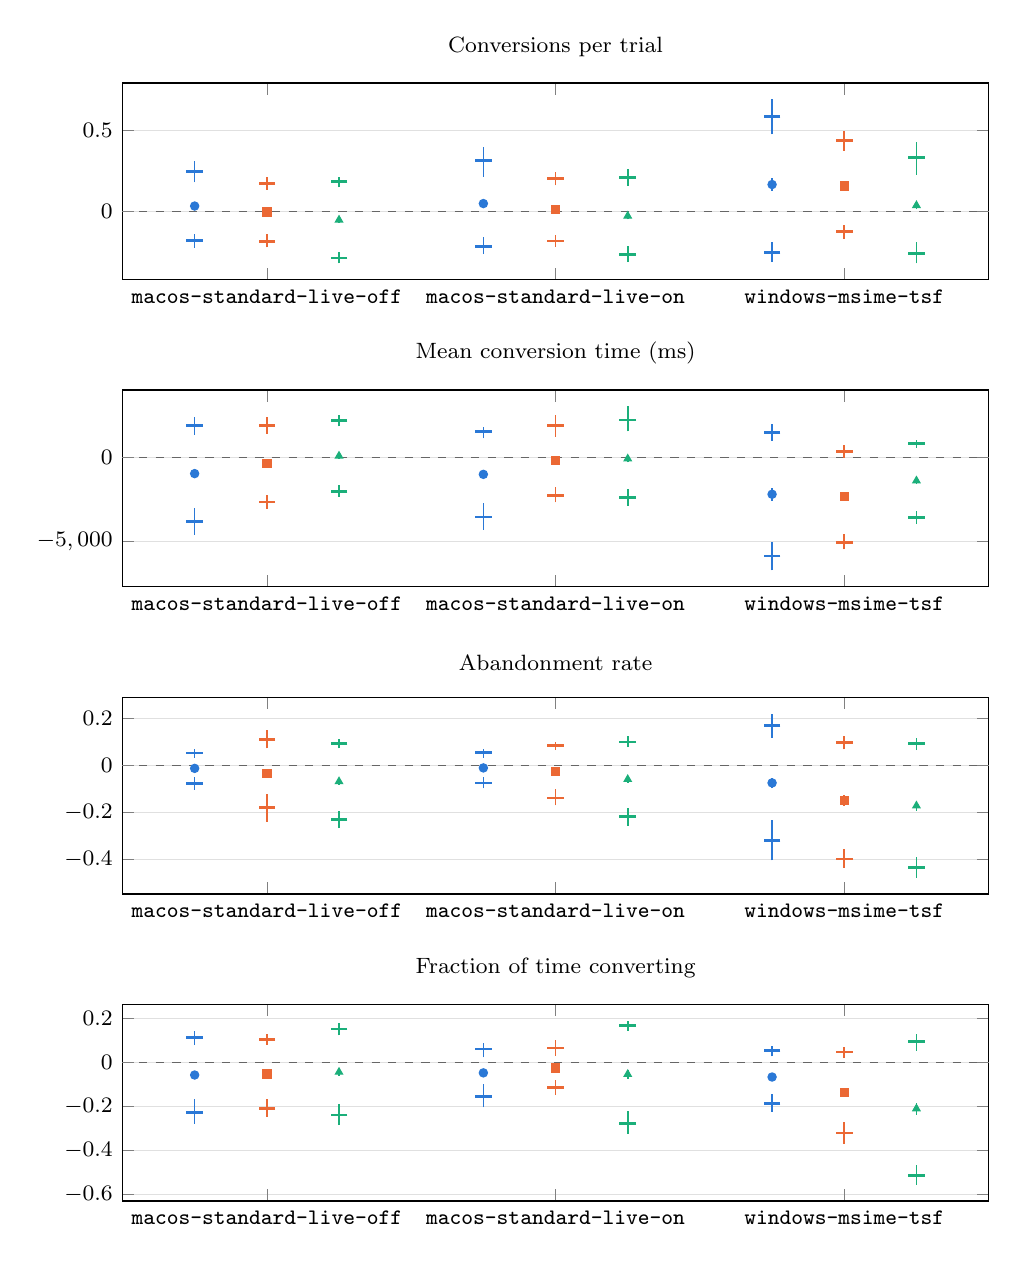
\begin{tikzpicture}
\begin{groupplot}[group style={group size=1 by 4, vertical sep=1.4cm}, fig panel, fig zero, scale only axis, width=11cm, height=2.5cm, xtick={1,2,3}, xticklabels={\texttt{macos-standard-live-off},\texttt{macos-standard-live-on},\texttt{windows-msime-tsf}}, xmin=0.5, xmax=3.5]
\nextgroupplot[title={Conversions per trial}, legend to name=fig:text-agreement:legend, legend columns=4]
\addlegendimage{fig slow, fig point}
\addlegendentry{slow}
\addlegendimage{fig mid, fig point}
\addlegendentry{mid}
\addlegendimage{fig fast, fig point}
\addlegendentry{fast}
\addlegendimage{black, fig limit}
\addlegendentry{limit of agreement}
\addplot[forget plot, fig interval, fig slow] table[row sep=\\] {x y\\0.75 0.0137968\\0.75 0.0565787\\0.75 nan\\0.75 -0.220809\\0.75 -0.136131\\0.75 nan\\0.75 0.179633\\0.75 0.308846\\0.75 nan\\1.75 0.0248955\\1.75 0.0760574\\1.75 nan\\1.75 -0.261969\\1.75 -0.15442\\1.75 nan\\1.75 0.215324\\1.75 0.399236\\1.75 nan\\2.75 0.127467\\2.75 0.209161\\2.75 nan\\2.75 -0.310034\\2.75 -0.187389\\2.75 nan\\2.75 0.474696\\2.75 0.690745\\2.75 nan\\};
\addplot[forget plot, fig slow, fig limit] table[row sep=\\] {x y\\0.75 -0.178767\\1.75 -0.214465\\2.75 -0.250327\\0.75 0.247509\\1.75 0.313681\\2.75 0.583864\\};
\addplot[forget plot, fig slow, fig point] table[row sep=\\] {x y\\0.75 0.0343712\\1.75 0.049608\\2.75 0.166768\\};
\addplot[forget plot, fig interval, fig mid] table[row sep=\\] {x y\\1 -0.0178577\\1 0.00922975\\1 nan\\1 -0.220274\\1 -0.137461\\1 nan\\1 0.133838\\1 0.215377\\1 nan\\2 -0.00826278\\2 0.0355079\\2 nan\\2 -0.217972\\2 -0.142543\\2 nan\\2 0.161662\\2 0.245401\\2 nan\\3 0.134052\\3 0.179142\\3 nan\\3 -0.166346\\3 -0.0797757\\3 nan\\3 0.375232\\3 0.494742\\3 nan\\};
\addplot[forget plot, fig mid, fig limit] table[row sep=\\] {x y\\1 -0.181472\\2 -0.181242\\3 -0.12198\\1 0.174879\\2 0.206037\\3 0.436799\\};
\addplot[forget plot, fig mid, fig point] table[row sep=\\] {x y\\1 -0.0032967\\2 0.0123978\\3 0.15741\\};
\addplot[forget plot, fig interval, fig fast] table[row sep=\\] {x y\\1.25 -0.0684778\\1.25 -0.0321009\\1.25 nan\\1.25 -0.318354\\1.25 -0.247791\\1.25 nan\\1.25 0.149591\\1.25 0.214642\\1.25 nan\\2.25 -0.0471251\\2.25 -0.00645323\\2.25 nan\\2.25 -0.311293\\2.25 -0.214478\\2.25 nan\\2.25 0.159809\\2.25 0.259746\\2.25 nan\\3.25 0.0132262\\3.25 0.0645655\\3.25 nan\\3.25 -0.318555\\3.25 -0.185716\\3.25 nan\\3.25 0.225438\\3.25 0.43123\\3.25 nan\\};
\addplot[forget plot, fig fast, fig limit] table[row sep=\\] {x y\\1.25 -0.28563\\2.25 -0.262432\\3.25 -0.256792\\1.25 0.18388\\2.25 0.20955\\3.25 0.333511\\};
\addplot[forget plot, fig fast, fig point] table[row sep=\\] {x y\\1.25 -0.0508751\\2.25 -0.0264411\\3.25 0.0383598\\};
\nextgroupplot[title={Mean conversion time (ms)}]
\addplot[forget plot, fig interval, fig slow] table[row sep=\\] {x y\\0.75 -1261.86\\0.75 -691.009\\0.75 nan\\0.75 -4610.86\\0.75 -3041.94\\0.75 nan\\0.75 1357.61\\0.75 2423.44\\0.75 nan\\1.75 -1287.48\\1.75 -769.965\\1.75 nan\\1.75 -4315.51\\1.75 -2725.52\\1.75 nan\\1.75 1129.49\\1.75 1824.28\\1.75 nan\\2.75 -2579.08\\2.75 -1852.1\\2.75 nan\\2.75 -6748.57\\2.75 -5032.46\\2.75 nan\\2.75 984.201\\2.75 1976.19\\2.75 nan\\};
\addplot[forget plot, fig slow, fig limit] table[row sep=\\] {x y\\0.75 -3841.17\\1.75 -3552.51\\2.75 -5878.05\\0.75 1899.84\\1.75 1523.73\\2.75 1475.88\\};
\addplot[forget plot, fig slow, fig point] table[row sep=\\] {x y\\0.75 -970.666\\1.75 -1014.39\\2.75 -2201.08\\};
\addplot[forget plot, fig interval, fig mid] table[row sep=\\] {x y\\1 -557.669\\1 -178.966\\1 nan\\1 -3073.94\\1 -2240.67\\1 nan\\1 1413.68\\1 2389.74\\1 nan\\2 -393.016\\2 45.8076\\2 nan\\2 -2690.07\\2 -1764.42\\2 nan\\2 1222.49\\2 2540.43\\2 nan\\3 -2571.92\\3 -2116.47\\3 nan\\3 -5490.45\\3 -4574.81\\3 nan\\3 -25.5713\\3 709.108\\3 nan\\};
\addplot[forget plot, fig mid, fig limit] table[row sep=\\] {x y\\1 -2662.93\\2 -2254.78\\3 -5058.22\\1 1905.33\\2 1907.89\\3 371.489\\};
\addplot[forget plot, fig mid, fig point] table[row sep=\\] {x y\\1 -378.801\\2 -173.443\\3 -2343.37\\};
\addplot[forget plot, fig interval, fig fast] table[row sep=\\] {x y\\1.25 -94.6766\\1.25 257.511\\1.25 nan\\1.25 -2338.43\\1.25 -1660.41\\1.25 nan\\1.25 1845.51\\1.25 2514.94\\1.25 nan\\2.25 -296.116\\2.25 156.763\\2.25 nan\\2.25 -2895.36\\2.25 -1883.35\\2.25 nan\\2.25 1547.61\\2.25 3036.08\\2.25 nan\\3.25 -1600.93\\3.25 -1207.2\\3.25 nan\\3.25 -3979.15\\3.25 -3198.67\\3.25 nan\\3.25 565.278\\3.25 1042.63\\3.25 nan\\};
\addplot[forget plot, fig fast, fig limit] table[row sep=\\] {x y\\1.25 -2025.32\\2.25 -2384.61\\3.25 -3604.34\\1.25 2196.62\\2.25 2221.25\\3.25 814.444\\};
\addplot[forget plot, fig fast, fig point] table[row sep=\\] {x y\\1.25 85.6454\\2.25 -81.6779\\3.25 -1394.95\\};
\nextgroupplot[title={Abandonment rate}]
\addplot[forget plot, fig interval, fig slow] table[row sep=\\] {x y\\0.75 -0.0183359\\0.75 -0.00550392\\0.75 nan\\0.75 -0.103954\\0.75 -0.0466396\\0.75 nan\\0.75 0.0339079\\0.75 0.0695433\\0.75 nan\\1.75 -0.0162794\\1.75 -0.00358063\\1.75 nan\\1.75 -0.0974907\\1.75 -0.0464943\\1.75 nan\\1.75 0.0334953\\1.75 0.0702787\\1.75 nan\\2.75 -0.0974065\\2.75 -0.0521038\\2.75 nan\\2.75 -0.404381\\2.75 -0.231365\\2.75 nan\\2.75 0.118328\\2.75 0.222407\\2.75 nan\\};
\addplot[forget plot, fig slow, fig limit] table[row sep=\\] {x y\\0.75 -0.0775651\\1.75 -0.0740273\\2.75 -0.318412\\0.75 0.0542846\\1.75 0.0546118\\2.75 0.171065\\};
\addplot[forget plot, fig slow, fig point] table[row sep=\\] {x y\\0.75 -0.0116402\\1.75 -0.0097077\\2.75 -0.0736739\\};
\addplot[forget plot, fig interval, fig mid] table[row sep=\\] {x y\\1 -0.0468264\\1 -0.0222586\\1 nan\\1 -0.238715\\1 -0.120698\\1 nan\\1 0.0736147\\1 0.149951\\1 nan\\2 -0.0372833\\2 -0.0155313\\2 nan\\2 -0.169692\\2 -0.100276\\2 nan\\2 0.0664793\\2 0.0997035\\2 nan\\3 -0.171625\\3 -0.127335\\3 nan\\3 -0.435022\\3 -0.356656\\3 nan\\3 0.0691825\\3 0.127661\\3 nan\\};
\addplot[forget plot, fig mid, fig limit] table[row sep=\\] {x y\\1 -0.178358\\2 -0.13783\\3 -0.398436\\1 0.110083\\2 0.0856654\\3 0.0987183\\};
\addplot[forget plot, fig mid, fig point] table[row sep=\\] {x y\\1 -0.0341372\\2 -0.0260823\\3 -0.149859\\};
\addplot[forget plot, fig interval, fig fast] table[row sep=\\] {x y\\1.25 -0.0808639\\1.25 -0.0554578\\1.25 nan\\1.25 -0.266532\\1.25 -0.1935\\1.25 nan\\1.25 0.0736502\\1.25 0.113685\\1.25 nan\\2.25 -0.0728879\\2.25 -0.0449424\\2.25 nan\\2.25 -0.256723\\2.25 -0.180276\\2.25 nan\\2.25 0.0787637\\2.25 0.124625\\2.25 nan\\3.25 -0.192895\\3.25 -0.148815\\3.25 nan\\3.25 -0.477632\\3.25 -0.389368\\3.25 nan\\3.25 0.0663391\\3.25 0.118487\\3.25 nan\\};
\addplot[forget plot, fig fast, fig limit] table[row sep=\\] {x y\\1.25 -0.230252\\2.25 -0.217832\\3.25 -0.436111\\1.25 0.0948428\\2.25 0.101054\\3.25 0.0937557\\};
\addplot[forget plot, fig fast, fig point] table[row sep=\\] {x y\\1.25 -0.0677045\\2.25 -0.058389\\3.25 -0.171178\\};
\nextgroupplot[title={Fraction of time converting}]
\addplot[forget plot, fig interval, fig slow] table[row sep=\\] {x y\\0.75 -0.0727727\\0.75 -0.0419352\\0.75 nan\\0.75 -0.278801\\0.75 -0.16807\\0.75 nan\\0.75 0.0801202\\0.75 0.14193\\0.75 nan\\1.75 -0.0583606\\1.75 -0.0365913\\1.75 nan\\1.75 -0.203414\\1.75 -0.0991124\\1.75 nan\\1.75 0.0236671\\1.75 0.0902096\\1.75 nan\\2.75 -0.0757142\\2.75 -0.0555747\\2.75 nan\\2.75 -0.223332\\2.75 -0.144563\\2.75 nan\\2.75 0.0279813\\2.75 0.0763184\\2.75 nan\\};
\addplot[forget plot, fig slow, fig limit] table[row sep=\\] {x y\\0.75 -0.226043\\1.75 -0.15533\\2.75 -0.18638\\0.75 0.113162\\1.75 0.062031\\2.75 0.0552155\\};
\addplot[forget plot, fig slow, fig point] table[row sep=\\] {x y\\0.75 -0.0564405\\1.75 -0.0466495\\2.75 -0.0655823\\};
\addplot[forget plot, fig interval, fig mid] table[row sep=\\] {x y\\1 -0.0647352\\1 -0.037892\\1 nan\\1 -0.24751\\1 -0.166924\\1 nan\\1 0.0818906\\1 0.129647\\1 nan\\2 -0.0310215\\2 -0.0169641\\2 nan\\2 -0.148586\\2 -0.0769847\\2 nan\\2 0.0300855\\2 0.101428\\2 nan\\3 -0.156174\\3 -0.116918\\3 nan\\3 -0.369001\\3 -0.270129\\3 nan\\3 0.0200337\\3 0.0721026\\3 nan\\};
\addplot[forget plot, fig mid, fig limit] table[row sep=\\] {x y\\1 -0.209188\\2 -0.114821\\3 -0.320378\\1 0.107008\\2 0.0667371\\3 0.0483024\\};
\addplot[forget plot, fig mid, fig point] table[row sep=\\] {x y\\1 -0.0510901\\2 -0.0240419\\3 -0.136038\\};
\addplot[forget plot, fig interval, fig fast] table[row sep=\\] {x y\\1.25 -0.0598186\\1.25 -0.0271184\\1.25 nan\\1.25 -0.28509\\1.25 -0.187262\\1.25 nan\\1.25 0.124557\\1.25 0.181799\\1.25 nan\\2.25 -0.074464\\2.25 -0.0333915\\2.25 nan\\2.25 -0.323565\\2.25 -0.22158\\2.25 nan\\2.25 0.145255\\2.25 0.191593\\2.25 nan\\3.25 -0.238401\\3.25 -0.181827\\3.25 nan\\3.25 -0.556206\\3.25 -0.468247\\3.25 nan\\3.25 0.0544072\\3.25 0.129845\\3.25 nan\\};
\addplot[forget plot, fig fast, fig limit] table[row sep=\\] {x y\\1.25 -0.23921\\2.25 -0.275999\\3.25 -0.514636\\1.25 0.153092\\2.25 0.170183\\3.25 0.0950716\\};
\addplot[forget plot, fig fast, fig point] table[row sep=\\] {x y\\1.25 -0.043059\\2.25 -0.0529079\\3.25 -0.209782\\};
\end{groupplot}
\end{tikzpicture}
\caption{Per-text agreement of the four measures per cell and speed in the primary scope: the bias (marks) and the lower and upper limits of agreement (dashes) of the per-text difference (observation minus reference), each with a 95\% interval that resamples blocks. The values hold for this design's numbers of trials per text and are not compared between speeds, and the values of the Windows cell estimate the agreement with a different construct and are not compared with those of the macOS cells; a measure with no text in the scope is not drawn. Table~\ref{tab:text-agreement} gives the values with ICC(A,1). The figure is drawn from the result files by code written with the assistance of an AI tool and reviewed by the author (AI declaration)}
\label{fig:text-agreement}
\end{figure}


% Section 8 of the manuscript: text recoverability (question 4). The method is stated first, as the outline
% requires; it follows sections 6.8 and 10.7 of the frozen registration. The results are written from the result
% files e2_closed_set_<cell>.json and e2_open_set_<cell>.json after the analysis.

\section{Results: text recoverability}
\label{sec:recoverability}

\subsection{Method}
\label{sec:recoverability-method}

The text-recoverability study asked how much of the typed text the key rows of a published log still reveal. Two
attacks were run on the observation log of each cell separately, with the plan, the procedures and the settings that
built it; the attacks refused a log whose plan or settings did not match. Both read the category and the time of
every key row of a press and nothing else: they did not use the session rows or the rows of key releases, and no plan
sent a modifier key, so on Windows, where modifier keys produce rows, no such row was read either. The ground truth of
an attack was the reading that was typed,
not the original sentence. The trials of scenario S12, whose phrase is a generated kana string, were not scored. When
every block is scored this leaves 2{,}925 trials with live conversion on and 2{,}700 with it off on macOS, and 2{,}700
on Windows.

\paragraph{Assigning presses to trials.} Both attacks assign the observed presses to the trials in plan order, block
by block. A block is placed where its marker of four arrow presses and all its trials match the observed presses. A
block whose observed presses do not agree with the plan (a press missing, added or changed) is not scored: its trials
are counted as unscored, and the assignment continues with the next block that matches, so that a difference loses
only the block that holds it. This behaviour was checked by the self-test of the code on the cases it constructs, not
proved in general. Before each freeze the assignment, without any attack, was run on the key rows of the pilots: it
scored every block of the three macOS pilot runs that used the arrow-key marker (15 blocks, 282 trials) and of the
seven Windows pilot runs (27 blocks, 429 trials) and left no press unassigned. These logs had no missing or added
press, so the check shows that clean logs are scored whole; it does not exercise the recovery after a difference.
Accuracies and error rates are computed over the scored trials, and the numbers of unscored blocks and trials are
reported per cell.

\paragraph{Closed set.} For each trial the attacker was given $K$ candidate phrases, the true one and $K-1$ decoys
drawn from the phrases that the trial's scenario could have produced (excluding phrases with the same reading). It
knew the scenario, the system, the speed, the generator, the procedures and the settings, generated the expected log
of each candidate with the same generator, and chose the candidate whose expected log was closest to the observed
one. $K$ was 10, 100 and 1{,}000. The attack was repeated on six feature sets that remove information from the log:
exact times and the lengths of runs of letter keys (\emph{all}), no times (\emph{no time}), no run lengths (\emph{no
runs}), times in 1-second bins (\emph{1-s bins}), 1-second bins without run lengths (\emph{1-s bin counts}), and
neither times nor run lengths (\emph{counts only}). Because an attacker given a detailed log can always discard
information, the accuracy of a feature set is the maximum over that set and every coarser set derived from it. The
accuracy is reported with its Wilson interval and, descriptively, with a 95\% percentile interval from 2{,}000
resamples of whole blocks, together with the chance level $1/K$, the mean rank of the true phrase and, without an
interval, the accuracy of each feature set alone per scenario and per speed.

\paragraph{The near-chance rule.} The synthetic key intervals were drawn independently of the keys, so the logs carry
none of the timing structure of human typing, neither the timing of particular key pairs nor the pauses between words
and phrases. The accuracy on the four feature sets that keep any time is therefore reported as an estimate only and
does not enter the recommendation, which considers the two sets that keep no time (\emph{no time} and its coarsening
\emph{counts only}). The accuracy of a feature set is near chance at $K=10$ or $K=100$ when the upper end of its 95\%
Wilson interval is at most $2/K$. A set is near chance for the recommendation when it is near chance at both values of
$K$ in both macOS cells, and the recommended granularity is the more detailed of the two sets that is near chance in
this sense; if neither is, no granularity is recommended, and this is reported. At $K=1{,}000$ an attack at the chance
level would rarely be judged near chance at the planned numbers of trials, so $K=1{,}000$ is reported descriptively
and is not part of the rule. The probability of the judgement at the planned numbers of trials was fixed in the
registration and is given with the results (Table~\ref{tab:nearchance}). The margin of $2/K$ and the values of $K$
are choices of the design, not derived from a criterion of privacy. The Wilson interval treats trials as independent;
with dependence within a block the rule is met more easily than it should be, which is why the block-resampled
interval is reported next to it. The recommendation was decided from the two macOS cells. The same judgement was made
for the Windows cell and, where it does not hold, is reported as a qualification of the recommendation for logs
recorded on Windows; it does not change the recommendation.

\paragraph{Open set.} A second attacker saw only the categories of the key presses and, with a character language
model, searched for the kana string that Romaji input would spell with exactly the observed letter keys and the
observed punctuation, maximising its probability. Two levels of knowledge were evaluated. The first knew nothing of
the genre beyond the frequency of single characters (a character unigram model estimated from the training phrases).
The second knew the genre but not the individual work: a character trigram model with Witten--Bell smoothing
\citep{wittenbell1991}, trained on the corpus with the whole works of the evaluation phrases held out (three of the
twelve works, drawn with the seed, holding at least a fifth of the phrases; a training phrase with the reading of an
evaluation phrase was removed). A stronger attacker of the second level, for which the corpus was split by phrase
instead of by work, is reported alongside it. The baseline was the same model without the log, drawing a string from
its prior while knowing either the number of segments or the true length. Reported are the character error rate of
the attack and of the baseline, their paired difference, and the difference from a negative control in which each
trial is decoded from another trial's observation, each with a percentile interval from resampling whole blocks. The
open set does not enter the rule; it is reported next to the recommendation as a second view of what the lengths of
letter runs, which the \emph{no time} set keeps, reveal.

\paragraph{What is not evaluated.} The rule judges the identification of one phrase among $K$ candidates in one
trial. Combining several trials of one writer, matching a log against known final texts, and identifying a writer
from the timing of a log are not evaluated, and no log is described as safe to publish. The session rows carry their
times and durations in milliseconds and could undo the coarsening of the key rows; they were not given to the attacks,
and publishing them is not evaluated. Neither are the rows of key releases or, on Windows, the rows of modifier keys.
The feature sets that keep time are reported as estimates only, so whether key rows with times can be published is
not judged, and granularities between milliseconds and 1-second bins were not evaluated. Neither attack is
claimed to be the strongest possible. The attacker knew the generator and the procedures, and the input had no
typing errors; these conditions are expected to favour identification, which is stated as an expectation, not as a
result.

\subsection{Results}
\label{sec:recoverability-results}

Every block of every cell was scored (\rv{macos-standard-live-off.q4.unscored} unscored with live conversion off,
\rv{macos-standard-live-on.q4.unscored} with it on, \rv{windows-msime-tsf.q4.unscored} on Windows), so the rule was
applied to the planned numbers of trials, whose properties Table~\ref{tab:nearchance} gives.

\paragraph{Closed set and the recommendation.} Table~\ref{tab:closed-set} gives the accuracy of the two feature sets
that keep no time. With live conversion off, the accuracy of \texttt{no\_time} was
\rv{macos-standard-live-off.q4.no_time.k10.acc} at $K = 10$ and \rv{macos-standard-live-off.q4.no_time.k100.acc} at
$K = 100$; with it on, \rv{macos-standard-live-on.q4.no_time.k10.acc} and
\rv{macos-standard-live-on.q4.no_time.k100.acc}. The accuracy of \texttt{counts\_only}, the maximum over that set and
the set derived from it, was \rv{macos-standard-live-off.q4.counts_only.k10.acc} and
\rv{macos-standard-live-off.q4.counts_only.k100.acc} with live conversion off and
\rv{macos-standard-live-on.q4.counts_only.k10.acc} and \rv{macos-standard-live-on.q4.counts_only.k100.acc} with it on.
In both macOS cells the upper end of every one of these Wilson intervals lies above $2/K$, so neither set is near chance
under the registered rule (\texttt{no\_time}: \rv{macos-standard-live-off.q4.no_time.near} and
\rv{macos-standard-live-on.q4.no_time.near}; \texttt{counts\_only}: \rv{macos-standard-live-off.q4.counts_only.near}
and \rv{macos-standard-live-on.q4.counts_only.near}), and the recommended granularity is \rv{q4.recommendation}: no
granularity of the key rows is recommended. The rule judges the identification of one phrase among $K$ candidates in
one trial; this result is not a judgement of the privacy of a log.

On Windows the same judgement gives: \rv{q4.windows.qualification}. The Windows accuracies of the two sets equal those of
the macOS cell with live conversion off to the reported precision. The two plans were generated from the same seed and
share every trial's block, scenario, speed, phrase and times; their presses differ only in S2, where the macOS
procedure presses one Return more, and in S4, where the Windows procedure presses one Escape more (deviation D1), and
the presses of letters, digits and punctuation are the same in every trial. The Windows judgement is therefore not an
independent replication of the macOS one for these sets.

Figure~\ref{fig:closed-set} shows every feature set at every $K$, and the supplement gives their values, with the
accuracy per speed and scenario. The sets that keep time
are estimates only: the synthetic intervals carry none of the timing structure of human typing, and these sets enter
neither the judgement nor the recommendation.

\paragraph{Open set.} Table~\ref{tab:open-set} gives the character error rate of the attack and of the prior-only
baseline, their difference (gain), and the gain over the shuffled control, in which each trial is decoded from another
trial's observation. With the number of segments known, the gain of K1 was
\rv{macos-standard-live-off.q4.open.K1.count.gain} with live conversion off and
\rv{macos-standard-live-on.q4.open.K1.count.gain} with it on, and its gain over the shuffled control
\rv{macos-standard-live-off.q4.open.K1.count.gainvsshuffled} and \rv{macos-standard-live-on.q4.open.K1.count.gainvsshuffled};
for K1+ the gain over the shuffled control was \rv{macos-standard-live-off.q4.open.K1plus.count.gainvsshuffled} and
\rv{macos-standard-live-on.q4.open.K1plus.count.gainvsshuffled}, and for K0
\rv{macos-standard-live-off.q4.open.K0.count.gainvsshuffled} and \rv{macos-standard-live-on.q4.open.K0.count.gainvsshuffled}.
With the true length known, the gain of K1 over the baseline was \rv{macos-standard-live-off.q4.open.K1.true.gain} and
\rv{macos-standard-live-on.q4.open.K1.true.gain}. The open-set file of the Windows cell is byte-identical to that of the
macOS cell with live conversion off: the attack decodes the letter keys and the punctuation, which the two plans share,
and every press other than the input-mode keys reached the log in both cells. The open set does not enter the rule;
it is a second view of what the letter-run lengths kept by \texttt{no\_time} reveal, for these attacks.

% Generated by manuscript/tools/results_tables.py from the result files; do not edit by hand.
\begin{sidewaystable}[p]
\caption{Closed-set identification for the two feature sets that keep no time: the accuracy (the maximum over the set and the sets derivable from it) with its Wilson interval and, descriptively, the interval that resamples blocks; a set is near chance at K when the upper end of the Wilson interval is at most 2/K, and near chance for the rule when it is so at both K = 10 and K = 100. The recommendation is decided from the two macOS cells; the Windows judgement is reported as its qualification; --: no value}
\label{tab:closed-set}
\begin{tabular}{L{0.20}L{0.12}L{0.06}L{0.07}L{0.22}L{0.15}L{0.07}L{0.10}}
\toprule
Cell & Feature set & K & Trials & Accuracy & Block interval & 2/K & Near chance \\
\midrule
macos-standard-live-off & \texttt{no\_time} & 10 & 2{,}700 & 0.902 [0.890, 0.913] & 0.891, 0.913 & 0.200 & no \\
 & \texttt{no\_time} & 100 & 2{,}700 & 0.421 [0.403, 0.440] & 0.408, 0.442 & 0.020 & no \\
 & \texttt{counts\_only} & 10 & 2{,}700 & 0.902 [0.890, 0.913] & 0.890, 0.913 & 0.200 & no \\
 & \texttt{counts\_only} & 100 & 2{,}700 & 0.421 [0.403, 0.440] & 0.403, 0.440 & 0.020 & no \\
macos-standard-live-on & \texttt{no\_time} & 10 & 2{,}925 & 0.907 [0.896, 0.917] & 0.897, 0.917 & 0.200 & no \\
 & \texttt{no\_time} & 100 & 2{,}925 & 0.435 [0.417, 0.453] & 0.418, 0.454 & 0.020 & no \\
 & \texttt{counts\_only} & 10 & 2{,}925 & 0.907 [0.896, 0.917] & 0.896, 0.917 & 0.200 & no \\
 & \texttt{counts\_only} & 100 & 2{,}925 & 0.435 [0.417, 0.453] & 0.417, 0.453 & 0.020 & no \\
windows-msime-tsf & \texttt{no\_time} & 10 & 2{,}700 & 0.902 [0.890, 0.913] & 0.891, 0.913 & 0.200 & no \\
 & \texttt{no\_time} & 100 & 2{,}700 & 0.421 [0.403, 0.440] & 0.408, 0.442 & 0.020 & no \\
 & \texttt{counts\_only} & 10 & 2{,}700 & 0.902 [0.890, 0.913] & 0.890, 0.913 & 0.200 & no \\
 & \texttt{counts\_only} & 100 & 2{,}700 & 0.421 [0.403, 0.440] & 0.403, 0.440 & 0.020 & no \\
\midrule
\multicolumn{8}{l}{Recommendation from the two macOS cells: none} \\
\bottomrule
\end{tabular}
\end{sidewaystable}

% Generated by manuscript/tools/results_tables.py from the result files; do not edit by hand.
\begin{figure}[t]
\centering
\pgfplotslegendfromname{fig:closed-set:legend}\par\medskip
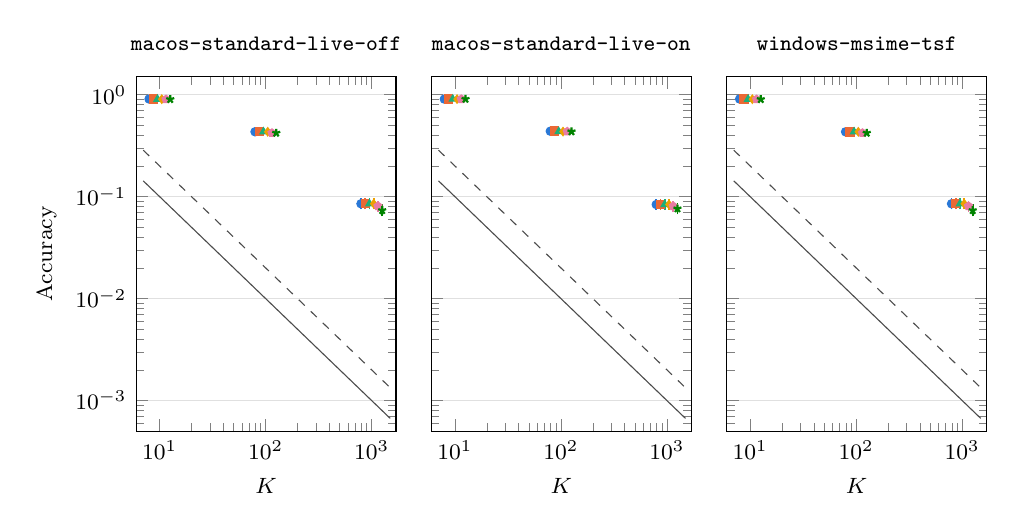
\begin{tikzpicture}
\begin{groupplot}[group style={group size=3 by 1, horizontal sep=0.45cm, yticklabels at=edge left, ylabels at=edge left}, fig panel, xmode=log, ymode=log, xtick={10,100,1000}, xmin=6, xmax=1700, ymin=0.0005, ymax=1.5, scale only axis, width=3.3cm, height=4.5cm, xlabel={$K$}, ylabel={Accuracy}]
\nextgroupplot[title={\texttt{macos-standard-live-off}}, legend to name=fig:closed-set:legend, legend columns=4]
\addlegendimage{fig set1, fig point}
\addlegendentry{\texttt{all}}
\addlegendimage{fig set2, fig point}
\addlegendentry{\texttt{no\_runs}}
\addlegendimage{fig set3, fig point}
\addlegendentry{\texttt{bin1s}}
\addlegendimage{fig set4, fig point}
\addlegendentry{\texttt{bin1s\_count}}
\addlegendimage{fig set5, fig point}
\addlegendentry{\texttt{no\_time}}
\addlegendimage{fig set6, fig point}
\addlegendentry{\texttt{counts\_only}}
\addlegendimage{fig chance}
\addlegendentry{$1/K$}
\addlegendimage{fig margin}
\addlegendentry{$2/K$}
\addplot[forget plot, fig chance, domain=7:1500] {1/x};
\addplot[forget plot, fig margin, domain=7:1500] {2/x};
\addplot[forget plot, fig interval, fig set1] table[row sep=\\] {x y\\7.94328 0.897056\\7.94328 0.91882\\7.94328 nan\\79.4328 0.41475\\79.4328 0.452106\\79.4328 nan\\794.328 0.0752358\\794.328 0.0963132\\794.328 nan\\};
\addplot[forget plot, fig set1, fig point] table[row sep=\\] {x y\\7.94328 0.908519\\79.4328 0.433333\\794.328 0.0851852\\};
\addplot[forget plot, fig interval, fig set2] table[row sep=\\] {x y\\8.70964 0.897056\\8.70964 0.91882\\8.70964 nan\\87.0964 0.41475\\87.0964 0.452106\\87.0964 nan\\870.964 0.0752358\\870.964 0.0963132\\870.964 nan\\};
\addplot[forget plot, fig set2, fig point] table[row sep=\\] {x y\\8.70964 0.908519\\87.0964 0.433333\\870.964 0.0851852\\};
\addplot[forget plot, fig interval, fig set3] table[row sep=\\] {x y\\9.54993 0.893163\\9.54993 0.915316\\9.54993 nan\\95.4993 0.41475\\95.4993 0.452106\\95.4993 nan\\954.993 0.0752358\\954.993 0.0963132\\954.993 nan\\};
\addplot[forget plot, fig set3, fig point] table[row sep=\\] {x y\\9.54993 0.904815\\95.4993 0.433333\\954.993 0.0851852\\};
\addplot[forget plot, fig interval, fig set4] table[row sep=\\] {x y\\10.4713 0.893163\\10.4713 0.915316\\10.4713 nan\\104.713 0.41475\\104.713 0.452106\\104.713 nan\\1047.13 0.0752358\\1047.13 0.0963132\\1047.13 nan\\};
\addplot[forget plot, fig set4, fig point] table[row sep=\\] {x y\\10.4713 0.904815\\104.713 0.433333\\1047.13 0.0851852\\};
\addplot[forget plot, fig interval, fig set5] table[row sep=\\] {x y\\11.4815 0.890052\\11.4815 0.91251\\11.4815 nan\\114.815 0.40298\\114.815 0.440206\\114.815 nan\\1148.15 0.0710503\\1148.15 0.0916225\\1148.15 nan\\};
\addplot[forget plot, fig set5, fig point] table[row sep=\\] {x y\\11.4815 0.901852\\114.815 0.421481\\1148.15 0.0807407\\};
\addplot[forget plot, fig interval, fig set6] table[row sep=\\] {x y\\12.5893 0.890052\\12.5893 0.91251\\12.5893 nan\\125.893 0.40298\\125.893 0.440206\\125.893 nan\\1258.93 0.064095\\1258.93 0.083784\\1258.93 nan\\};
\addplot[forget plot, fig set6, fig point] table[row sep=\\] {x y\\12.5893 0.901852\\125.893 0.421481\\1258.93 0.0733333\\};
\nextgroupplot[title={\texttt{macos-standard-live-on}}]
\addplot[forget plot, fig chance, domain=7:1500] {1/x};
\addplot[forget plot, fig margin, domain=7:1500] {2/x};
\addplot[forget plot, fig interval, fig set1] table[row sep=\\] {x y\\7.94328 0.895585\\7.94328 0.916682\\7.94328 nan\\79.4328 0.421082\\79.4328 0.457027\\79.4328 nan\\794.328 0.0742589\\794.328 0.0943543\\794.328 nan\\};
\addplot[forget plot, fig set1, fig point] table[row sep=\\] {x y\\7.94328 0.906667\\79.4328 0.438974\\794.328 0.0837607\\};
\addplot[forget plot, fig interval, fig set2] table[row sep=\\] {x y\\8.70964 0.895585\\8.70964 0.916682\\8.70964 nan\\87.0964 0.421082\\87.0964 0.457027\\87.0964 nan\\870.964 0.0742589\\870.964 0.0943543\\870.964 nan\\};
\addplot[forget plot, fig set2, fig point] table[row sep=\\] {x y\\8.70964 0.906667\\87.0964 0.438974\\870.964 0.0837607\\};
\addplot[forget plot, fig interval, fig set3] table[row sep=\\] {x y\\9.54993 0.895585\\9.54993 0.916682\\9.54993 nan\\95.4993 0.417343\\95.4993 0.453254\\95.4993 nan\\954.993 0.0742589\\954.993 0.0943543\\954.993 nan\\};
\addplot[forget plot, fig set3, fig point] table[row sep=\\] {x y\\9.54993 0.906667\\95.4993 0.435214\\954.993 0.0837607\\};
\addplot[forget plot, fig interval, fig set4] table[row sep=\\] {x y\\10.4713 0.895585\\10.4713 0.916682\\10.4713 nan\\104.713 0.417343\\104.713 0.453254\\104.713 nan\\1047.13 0.0742589\\1047.13 0.0943543\\1047.13 nan\\};
\addplot[forget plot, fig set4, fig point] table[row sep=\\] {x y\\10.4713 0.906667\\104.713 0.435214\\1047.13 0.0837607\\};
\addplot[forget plot, fig interval, fig set5] table[row sep=\\] {x y\\11.4815 0.895585\\11.4815 0.916682\\11.4815 nan\\114.815 0.417343\\114.815 0.453254\\114.815 nan\\1148.15 0.071355\\1148.15 0.0911124\\1148.15 nan\\};
\addplot[forget plot, fig set5, fig point] table[row sep=\\] {x y\\11.4815 0.906667\\114.815 0.435214\\1148.15 0.0806838\\};
\addplot[forget plot, fig interval, fig set6] table[row sep=\\] {x y\\12.5893 0.895585\\12.5893 0.916682\\12.5893 nan\\125.893 0.417343\\125.893 0.453254\\125.893 nan\\1258.93 0.067168\\1258.93 0.0864222\\1258.93 nan\\};
\addplot[forget plot, fig set6, fig point] table[row sep=\\] {x y\\12.5893 0.906667\\125.893 0.435214\\1258.93 0.0762393\\};
\nextgroupplot[title={\texttt{windows-msime-tsf}}]
\addplot[forget plot, fig chance, domain=7:1500] {1/x};
\addplot[forget plot, fig margin, domain=7:1500] {2/x};
\addplot[forget plot, fig interval, fig set1] table[row sep=\\] {x y\\7.94328 0.897056\\7.94328 0.91882\\7.94328 nan\\79.4328 0.414382\\79.4328 0.451735\\79.4328 nan\\794.328 0.0752358\\794.328 0.0963132\\794.328 nan\\};
\addplot[forget plot, fig set1, fig point] table[row sep=\\] {x y\\7.94328 0.908519\\79.4328 0.432963\\794.328 0.0851852\\};
\addplot[forget plot, fig interval, fig set2] table[row sep=\\] {x y\\8.70964 0.897056\\8.70964 0.91882\\8.70964 nan\\87.0964 0.414382\\87.0964 0.451735\\87.0964 nan\\870.964 0.0752358\\870.964 0.0963132\\870.964 nan\\};
\addplot[forget plot, fig set2, fig point] table[row sep=\\] {x y\\8.70964 0.908519\\87.0964 0.432963\\870.964 0.0851852\\};
\addplot[forget plot, fig interval, fig set3] table[row sep=\\] {x y\\9.54993 0.893163\\9.54993 0.915316\\9.54993 nan\\95.4993 0.414382\\95.4993 0.451735\\95.4993 nan\\954.993 0.0752358\\954.993 0.0963132\\954.993 nan\\};
\addplot[forget plot, fig set3, fig point] table[row sep=\\] {x y\\9.54993 0.904815\\95.4993 0.432963\\954.993 0.0851852\\};
\addplot[forget plot, fig interval, fig set4] table[row sep=\\] {x y\\10.4713 0.893163\\10.4713 0.915316\\10.4713 nan\\104.713 0.414382\\104.713 0.451735\\104.713 nan\\1047.13 0.0752358\\1047.13 0.0963132\\1047.13 nan\\};
\addplot[forget plot, fig set4, fig point] table[row sep=\\] {x y\\10.4713 0.904815\\104.713 0.432963\\1047.13 0.0851852\\};
\addplot[forget plot, fig interval, fig set5] table[row sep=\\] {x y\\11.4815 0.890052\\11.4815 0.91251\\11.4815 nan\\114.815 0.40298\\114.815 0.440206\\114.815 nan\\1148.15 0.0710503\\1148.15 0.0916225\\1148.15 nan\\};
\addplot[forget plot, fig set5, fig point] table[row sep=\\] {x y\\11.4815 0.901852\\114.815 0.421481\\1148.15 0.0807407\\};
\addplot[forget plot, fig interval, fig set6] table[row sep=\\] {x y\\12.5893 0.890052\\12.5893 0.91251\\12.5893 nan\\125.893 0.40298\\125.893 0.440206\\125.893 nan\\1258.93 0.064095\\1258.93 0.083784\\1258.93 nan\\};
\addplot[forget plot, fig set6, fig point] table[row sep=\\] {x y\\12.5893 0.901852\\125.893 0.421481\\1258.93 0.0733333\\};
\end{groupplot}
\end{tikzpicture}
\caption{Closed-set identification accuracy against the number of candidates $K$ for the six feature sets, per cell, with 95\% Wilson intervals; the accuracy of a set is the maximum over the set and the sets derivable from it. Solid line: the chance level $1/K$; dashed line: the margin $2/K$ of the near-chance rule, which judges \texttt{no\_time} and \texttt{counts\_only} at $K = 10$ and $100$; the sets that keep time are estimates only. The sets are set apart along $K$ for legibility; every point lies at $K = 10$, $100$ or $1{,}000$. Both axes are logarithmic. Table~\ref{tab:closed-set} gives the judgement. The figure is drawn from the result files by code written and reviewed with an AI tool (Claude) and checked by its tests; see the AI declaration}
\label{fig:closed-set}
\end{figure}

% Generated by manuscript/tools/results_tables.py from the result files; do not edit by hand.
\begin{sidewaystable}[p]
{\footnotesize
\caption{Open-set reconstruction per cell and attacker: character error rate (CER) of the attack and of the prior-only baseline, the gain (baseline CER minus attack CER) and the gain over the shuffled control (the CER of another trial's decoding minus the attack's), each with a block-clustered 95\% percentile interval. K1 holds out whole works, K1+ splits the corpus by phrase; the baseline knows the number of segments or the true length. Undecodable: trials for which no string fits; --: no value}
\label{tab:open-set}
\begin{tabular}{L{0.14}L{0.11}L{0.10}L{0.06}L{0.13}L{0.13}L{0.12}L{0.11}L{0.10}}
\toprule
Cell & Attacker & Length known & Trials & CER & Baseline CER & Gain & Gain over shuffled & Undecod\-able \\
\midrule
macos-standard-live-off & K0 & number of segments & 679 & 0.941 [0.937, 0.945] & 1.338 [1.281, 1.398] & 0.397 [0.337, 0.461] & 0.155 [0.124, 0.188] & 0 \\
 &  & true length & 679 & 0.941 [0.937, 0.945] & 0.968 [0.964, 0.971] & 0.027 [0.021, 0.032] & 0.155 [0.124, 0.188] & 0 \\
 & K1 & number of segments & 679 & 0.910 [0.903, 0.917] & 1.348 [1.282, 1.415] & 0.438 [0.371, 0.507] & 0.312 [0.260, 0.367] & 0 \\
 &  & true length & 679 & 0.910 [0.903, 0.917] & 0.961 [0.957, 0.965] & 0.051 [0.042, 0.059] & 0.312 [0.260, 0.367] & 0 \\
 & K1+ & number of segments & 544 & 0.913 [0.905, 0.922] & 1.353 [1.290, 1.422] & 0.439 [0.379, 0.508] & 0.334 [0.272, 0.401] & 0 \\
 &  & true length & 544 & 0.913 [0.905, 0.922] & 0.963 [0.958, 0.967] & 0.049 [0.041, 0.059] & 0.334 [0.272, 0.401] & 0 \\
 & K0 (split by phrase) & number of segments & 544 & 0.940 [0.935, 0.946] & 1.380 [1.319, 1.447] & 0.439 [0.377, 0.506] & 0.174 [0.134, 0.218] & 0 \\
 &  & true length & 544 & 0.940 [0.935, 0.946] & 0.969 [0.965, 0.972] & 0.028 [0.022, 0.035] & 0.174 [0.134, 0.218] & 0 \\
macos-standard-live-on & K0 & number of segments & 727 & 0.942 [0.938, 0.946] & 1.351 [1.292, 1.411] & 0.409 [0.348, 0.468] & 0.131 [0.105, 0.160] & 0 \\
 &  & true length & 727 & 0.942 [0.938, 0.946] & 0.967 [0.964, 0.970] & 0.026 [0.020, 0.031] & 0.131 [0.105, 0.160] & 0 \\
 & K1 & number of segments & 727 & 0.911 [0.903, 0.919] & 1.329 [1.273, 1.388] & 0.418 [0.359, 0.480] & 0.276 [0.232, 0.321] & 0 \\
 &  & true length & 727 & 0.911 [0.903, 0.919] & 0.964 [0.960, 0.968] & 0.053 [0.044, 0.062] & 0.276 [0.232, 0.321] & 0 \\
 & K1+ & number of segments & 580 & 0.916 [0.909, 0.924] & 1.329 [1.270, 1.394] & 0.413 [0.356, 0.471] & 0.290 [0.236, 0.349] & 0 \\
 &  & true length & 580 & 0.916 [0.909, 0.924] & 0.969 [0.965, 0.973] & 0.053 [0.044, 0.062] & 0.290 [0.236, 0.349] & 0 \\
 & K0 (split by phrase) & number of segments & 580 & 0.942 [0.937, 0.947] & 1.349 [1.292, 1.412] & 0.407 [0.349, 0.471] & 0.149 [0.116, 0.186] & 0 \\
 &  & true length & 580 & 0.942 [0.937, 0.947] & 0.967 [0.963, 0.971] & 0.025 [0.019, 0.030] & 0.149 [0.116, 0.186] & 0 \\
windows-msime-tsf & K0 & number of segments & 679 & 0.941 [0.937, 0.945] & 1.338 [1.281, 1.398] & 0.397 [0.337, 0.461] & 0.155 [0.124, 0.188] & 0 \\
 &  & true length & 679 & 0.941 [0.937, 0.945] & 0.968 [0.964, 0.971] & 0.027 [0.021, 0.032] & 0.155 [0.124, 0.188] & 0 \\
 & K1 & number of segments & 679 & 0.910 [0.903, 0.917] & 1.348 [1.282, 1.415] & 0.438 [0.371, 0.507] & 0.312 [0.260, 0.367] & 0 \\
 &  & true length & 679 & 0.910 [0.903, 0.917] & 0.961 [0.957, 0.965] & 0.051 [0.042, 0.059] & 0.312 [0.260, 0.367] & 0 \\
 & K1+ & number of segments & 544 & 0.913 [0.905, 0.922] & 1.353 [1.290, 1.422] & 0.439 [0.379, 0.508] & 0.334 [0.272, 0.401] & 0 \\
 &  & true length & 544 & 0.913 [0.905, 0.922] & 0.963 [0.958, 0.967] & 0.049 [0.041, 0.059] & 0.334 [0.272, 0.401] & 0 \\
 & K0 (split by phrase) & number of segments & 544 & 0.940 [0.935, 0.946] & 1.380 [1.319, 1.447] & 0.439 [0.377, 0.506] & 0.174 [0.134, 0.218] & 0 \\
 &  & true length & 544 & 0.940 [0.935, 0.946] & 0.969 [0.965, 0.972] & 0.028 [0.022, 0.035] & 0.174 [0.134, 0.218] & 0 \\
\bottomrule
\end{tabular}
}
\end{sidewaystable}


\begin{table}[t]
\caption{The near-chance rule: probability that a feature set is judged near chance when its true accuracy is $c/K$,
at the planned numbers of trials}
\label{tab:nearchance}
\begin{tabular}{rrrrrr}
\toprule
Trials & $K$ & $c=1$ & $c=1.5$ & $c=2$ & $c=3$ \\
\midrule
2{,}925 & 10 & 1.000 & 1.000 & 0.024 & 0.000 \\
2{,}925 & 100 & 0.994 & 0.487 & 0.020 & 0.000 \\
2{,}925 & 1{,}000 & 0.210 & 0.067 & 0.020 & 0.001 \\
2{,}700 & 10 & 1.000 & 1.000 & 0.025 & 0.000 \\
2{,}700 & 100 & 0.989 & 0.447 & 0.019 & 0.000 \\
2{,}700 & 1{,}000 & 0.067 & 0.017 & 0.004 & 0.000 \\
\bottomrule
\end{tabular}
\footnotetext{Binomial probability that the upper end of the Wilson interval is at most $2/K$, for the accuracy of
one feature set over the planned numbers of trials (2{,}925: live conversion on; 2{,}700: live conversion off and
Windows), as registered. For a set whose accuracy is the maximum over coarser sets the probability is at most this
value. If blocks are unscored, the rule is applied to the scored trials. The judgement of each cell is given in
Table~\ref{tab:closed-set}.}
\end{table}

% Section 9 of the manuscript: runtime cost (question 5). The method is stated first, as the outline requires; it
% follows sections 6.10 and 10.9 of the frozen registration and the description of the samplers in kit/e3/README.md.
% The results are written from the result files e3_macos.txt and e3_windows.txt after the analysis.

\section{Results: runtime cost}
\label{sec:cost}

\subsection{Method}
\label{sec:cost-method}

The cost of the logger to the machine was measured on each system under two conditions, one night each, for eight
hours at an interval of 30~s: \emph{idle}, in which the logger ran and nothing operated the machine, and
\emph{working}, in which the logger ran while the runner played the plan of one agreement cell (on macOS the plan with
live conversion on, which takes about 11.9~hours; on Windows the plan of the Windows cell, which takes 12 to
13~hours). In the working condition only the samples of the first eight hours were used. The conditions were measured
after the agreement cells of the same machine (Section~\ref{sec:method-cells}).

A sampler found the logger's process by its name and recorded, at every interval, its CPU and its resident memory; no
other process was listed and no window title was read. CPU is expressed on the basis that one core is 100\%. The two
systems measure differently. On macOS the CPU value of a sample is the increase of the process's cumulative CPU time
divided by the increase of the wall-clock time, a mean over the whole interval, and the memory is the resident memory
that the system's process monitor reports. On Windows the CPU value is the processor time of the process over about
one second at the moment of reading, so a burst between two samples is not seen, and the memory is the working set.
For this reason the values are described within each system and are not compared between the systems.

Reported for each condition are the mean, median, 95th percentile and maximum of the CPU, the final resident memory,
and the least-squares slope of the resident memory in megabytes per hour. The two conditions are always reported
together and are not reduced to one figure. A condition with fewer than 480 usable samples or a window shorter than
four hours was insufficient and was run again on another night, as was a condition that was aborted, up to three
attempts in all; every attempt is reported. In the working condition the runs were checked by the stopping rule of the
agreement cells (Section~\ref{sec:method-checks}). On Windows a counter that cannot be read gives zero, so a working
condition in which every CPU sample was zero was treated as insufficient, because the logger processes the presses of
the plan; in the idle condition a true zero is possible, and such a condition is reported with this flag. Battery use
was not measured. The samples of both conditions are deposited; the observation log of the idle condition is not,
because the logger was started before the command that begins the sampling was typed, so that log holds a person's
key presses.

\subsection{Results}
\label{sec:cost-results}

The records of the runs hold one attempt of each condition on each system (the working conditions are in
Table~\ref{tab:attempts}), and every one had enough samples to be reported (Table~\ref{tab:cost}). On macOS the mean CPU of the
logger was \rv{macos.e3.idle.cpu.mean} in the idle condition and \rv{macos.e3.working.cpu.mean} in the working
condition; on Windows it was \rv{windows.e3.idle.cpu.mean} idle and \rv{windows.e3.working.cpu.mean} working (one core
is 100). The values of each system are read within that system (Section~\ref{sec:cost-method}); the table gives the
median, the 95th percentile and the maximum of the CPU, the final memory and its slope for each condition.

% Generated by manuscript/tools/results_tables.py from the result files; do not edit by hand.
\begin{sidewaystable}[p]
\caption{Runtime cost of the logger per system and condition: CPU of the logger (one core is 100) over the samples, its final resident memory (macOS) or working set (Windows) and the least-squares slope of it. The samplers of the two systems measure differently, so the values are read within each system and not compared between systems; --: not measured, or not to be quoted (section 6.10)}
\label{tab:cost}
\begin{tabular}{L{0.10}L{0.09}L{0.18}L{0.07}L{0.09}L{0.10}L{0.10}L{0.07}L{0.10}L{0.10}}
\toprule
System & Condition & Status & Mean & Median & 95th percentile & Maximum & Hours & Memory (MB) & Slope (MB/h) \\
\midrule
macOS & idle & measured & 0.32 & 0.32 & 0.35 & 0.38 & 7.99 & 5.0 & 0.00 \\
 & working & measured & 0.36 & 0.35 & 0.47 & 0.55 & 7.99 & 5.2 & -0.00 \\
Windows & idle & measured & 5.56 & 4.68 & 10.82 & 20.21 & 7.99 & 15.1 & 0.01 \\
 & working & measured & 5.37 & 4.66 & 10.84 & 15.51 & 7.99 & 16.3 & 0.09 \\
\bottomrule
\end{tabular}
\end{sidewaystable}


% Section 11 of the manuscript: the dataset.
% What is deposited, and under which rules, follows sections 3.1, 3.4, 6.10 and 10.10 of the registration,
% experiment/data.md, experiment/data.windows.md and the sections on raw logs of experiment/pilot-macos.md and
% experiment/pilot-windows.md. Values that are known only after the deposit are marked with \tbd.

\section{The dataset}
\label{sec:dataset}

The records of the measurement are released as a dataset of the calls that a reference input field received from the
input method under scripted input, with the presses sent and the logger's rows: a ground truth against which rules
that infer conversions from key presses can be evaluated, and a set of key logs whose typed phrases are known
(Section~\ref{sec:dataset-uses}). The dataset is synthetic input in one kind of reference input field per system.

\subsection{Contents}
\label{sec:dataset-contents}

The dataset has two parts that are kept apart (Table~\ref{tab:dataset}). The first holds the runs of the measurement,
made from the registered plans. The second holds the runs of the calibration pilots that meet the registered criteria
for deposit; they were made from other plans, with provisional settings (Section~\ref{sec:method-pilots}). For each run
the dataset holds the plan, the record of every press that the executor sent, the log of the reference input field,
the logger's log and the run manifest, which records the versions of the system, the input method and the programs and
the SHA-256 of every log. It further holds the samples of the runtime-cost study, the phrase corpus, the settings of
the generator and the seed, and the specification of the formats, so that every field can be read from the deposit
alone. The observation logs of the pilots include the session rows that were sealed during the pilots; they are
unsealed only to be deposited and were not analysed.

\begin{table}[t]
\caption{Contents of the dataset. The measurement runs and the calibration-pilot runs are separate parts}
\label{tab:dataset}
\begin{tabular}{L{0.20}L{0.40}L{0.20}L{0.20}}
\toprule
Record & What it holds & Measurement runs & Calibration-pilot runs \\
\midrule
Plan & Every trial's scenario, speed, phrase identifier, intended outcome and key schedule; the generator's settings by SHA-256 & Registered plan of each cell & Plans of the pilots \\
Record of presses sent & Every press and release as sent, with wall-clock and monotonic times; block markers; trial boundaries & Yes & Yes \\
Reference log & Calls that the reference input field received: kinds, lengths and times, key codes of key-downs, changes of focus; no text & Yes & Yes \\
Observation log & The logger's header, key rows and session rows & Yes & Yes, with the session rows that were sealed \\
Run manifest & Versions, settings, outcome of the checks of the front window, SHA-256 of every log & Yes & Yes \\
Runtime samples & CPU and memory of the logger at 30-second intervals, in the idle and the working condition & Yes & No \\
Phrase corpus & 1{,}800 public-domain phrases with their readings and the identifiers of the source works & Shared by both parts & \\
Generator settings and seed & The settings and procedures from which the plans were generated & Shared by both parts & \\
Format specification & The fields and the permitted values of every record & Shared by both parts & \\
Datasheet & Motivation, composition, collection, preprocessing, uses, distribution and maintenance & Shared by both parts & \\
\bottomrule
\end{tabular}
\end{table}

In the dimensions on which keystroke datasets differ, the dataset holds fixed phrases typed without errors or
corrections by a program; keys as fourteen categories in the logger's log, without key names, as key codes in the
reference log and as key names in the record of presses; times of presses and releases on both systems; events injected through the
interfaces of the operating system, not typed on a physical keyboard; and a JIS keyboard layout on both systems.

\subsection{How the records were produced and checked}
\label{sec:dataset-checks}

The records were produced by the procedure of Section~\ref{sec:method}. Right after each attempt, and before any
analysis, the stopping rule was applied to the run's logs and the plan of every measurement run was checked by hand
against the registration (Section~\ref{sec:method-checks}). At deposit, a packing command bundles only the manifest and
the four logs of a run, refuses a run whose files hold an absolute path, the path of the repository, a login name or home
directory given to it, or content in the reference or observation log, applies the stopping rule and the check of the content-free
format again, and refuses a run that fails or cannot be checked; it writes the files in a fixed order with fixed times,
so that packing twice gives the same archive, and prints the SHA-256 of the archive, which is recorded with the run.
The stopping rule exists so that no person's typing enters the data, and its blind spots are stated in the
registration and in Section~\ref{sec:limitations}.

\subsection{What was not deposited}
\label{sec:dataset-excluded}

A completed run that the stopping rule catches is not deposited, because its logs may hold a person's key presses. A
run that the runner aborted is deposited only if it passes the same checks or left neither a reference log nor an
observation log; one aborted inside a trial does not pass. The observation log of the idle condition of the runtime-cost
study is not deposited, because the logger was started before the command that begins the sampling was typed, so the
log holds a person's key presses; only its samples are deposited. The logs of the working condition are deposited under
the rules of the measurement runs \tbd{confirmed at deposit}. The Windows pilot runs with the second reference field are
not deposited, because that field received the key press that switches the input method on as a key-down, which the
stopping rule counts as a press from outside. The error output of the programs stays on the measuring machines, and
checks typed by hand were not runs of the runner and are not deposited. The table of attempts states for every start
of every run of a plan whether it was deposited, with the reason where these rules decide it
(Section~\ref{sec:results-attempts}).

\subsection{Uses}
\label{sec:dataset-uses}

The records support three uses from the deposit alone. (a) The calls that an input method makes to an input field, per
system and setting, can be examined as a basis for re-examining definitions of a conversion. (b) Another rule that
infers sessions from key presses can be evaluated against the same ground truth without new measurement, by applying it
to the record of presses sent or to the key rows of the logger's log; the prediction of this study
(Section~\ref{sec:method-prediction}) is a worked example. (c) How far a key log without text reveals the text can be
studied with the typed phrases known, as in Section~\ref{sec:recoverability}. Evaluating a logger that needs other
signals, such as the windows of the input method, is a use of the kit rather than of the dataset: it means running the
kit again, which does not reproduce the same reference, because the learning of the input method and the versions
differ. The dataset is not suited as a record of human writing, as a benchmark of natural typing, or for inferences
about writers.

\subsection{Distribution and maintenance}
\label{sec:dataset-distribution}

The dataset is deposited in Zenodo under the persistent identifier \tbd{DOI of the dataset}, with the data and
documents under the Creative Commons Attribution 4.0 licence and the code under the Apache License 2.0
\citep{dataset}. A datasheet in the form proposed by \citet{gebru2021}, which organises the description by the stages
of a dataset's life (motivation, composition, collection process, preprocessing, uses, distribution and maintenance), is
released with it \tbd{written at deposit}. The datasheet
states the terms of the corpus source: the phrases come from works whose copyright has expired, which the source
library allows to be copied and redistributed freely, asking that the information recorded in its files be kept
\citep{aozora,aozora-terms}; the corpus records the identifier of each source work, and the source works are listed
with the SHA-256 of the archives downloaded. Corrections will be released as new versions under the same concept
identifier, with a record of what changed; the contact for the dataset is the corresponding author.


\bibliography{references}

\end{document}
